% +--------------------------------------------------------------------+
% | Chapter 06 - Subgroup Discovery			   						   |
% +--------------------------------------------------------------------+

\graphicspath{{./_figures/06_sd/}}

\section{Introduction}\label{section:SD:introduction}
Data mining or Knowledge Discovery from Data (KDD) is defined as the automatic extraction of patterns representing knowledge implicitly stored or captured in data \cite{Fayyad1996}. Up to now, a wide variety of data mining techniques have been introduced and developed \cite{Han2012}. These techniques are usually divided into two types: exploratory and predictive. Exploratory data analysis focuses on searching relations between objects of a dataset (clustering, association rule mining...) whereas predictive data analysis aims to extract knowledge from discovered data with an intent to predict or classify unknown examples (classification, regression, time series, decision trees...). In this chapter, we are interested in Subgroup Discovery (SD), a data mining technique that lies between these two perspectives.


Subgroup Discovery was introduced for the first time in \cite{Klosgen1996,Wrobel1997} with the aim of obtaining interesting subgroups of a population of individuals, where this interest was defined as to be as large as possible and to have the most unusual statistical characteristics with respect to a property of interest.  Nowadays, this perspective is wider and there exist many interestingness criteria to identify relevant subgroups of data, which are quantified by different quality functions \cite{Atzmueller2015}. Subgroups are usually represented as conditional statements
$$\text{Condition} \Rightarrow \text{Target},$$
where ``Target'' is the variable of interest for the subgroup discovery task and ``Condition'' is the conjunction of features representing relations characterized by the value of Target. These rules should be simple enough to be understood by experts and the intention is that from these rules the expert can either confirm his/her intuitions or obtain unknown knowledge. Let us provide an example, assume that we have a dataset of houses for which we are interested in studying the variable ``Price'' in terms of other available variables like antiquity, area, number of rooms, distance to the sea, distance to the city center... Two possible interesting subgroups could be
$$R_1~:~(\text{Antiquity} = \text{High}) \text{ and } (\text{Area} = \text{High}) \Rightarrow \text{Price} = \text{Medium}, \quad$$
$$R_2~:~(\text{Area} = \text{Low}) \text{ and } (\text{Distance to City Center} = \text{Low}) \Rightarrow \text{Price} = \text{High}.$$
In this hypothetical example, $R_1$ and $R_2$ represent two subgroups of houses that have unusual characteristics with respect to the rest of the buildings in the dataset. Let us point out that, although in this example we have not explicitly explained how the rules $R_1$ and $R_2$ are modeled, we can have an idea of the type of knowledge we get from these rules. Indeed, this is the key characteristic of SD algorithms, to discover relations between a subset of features and a target variable in terms of a few, simple and interpretable rules.

The ideas explained above are the basis of SD but they are rather general, so to design an SD algorithm various elements have to be considered. Distinct decisions on these key elements result in different SD algorithms. The most relevant can be found hereunder \cite{Herrera2011}: 
\begin{itemize}
	\item \textit{Type of Target Variable}: Typically, an SD algorithm focuses on and is only valid for one type of target variable: binary, nominal or numerical.
	\item \textit{Description Language}: Subgroups are conceptually represented as rules, but there are many ways of modeling these rules. First, the type of logical proposition corresponding to the antecedent of the rule has to be chosen (conjunction/disjunction of literals, disjunctive/conjunctive normal form...). Second, the value of the feature variables has to be represented as a logical value (through an equality, inequality, fuzzy logic...). Finally, the conditional in the subgroup has to be modeled, i.e., how the rules are evaluated has to be specified.
	\item \textit{Quality Measures}: In order to rank subgroups in terms of their interestingness, there exist many quality measures in the literature linked to different objectives. In the surveys \cite{Herrera2011,Atzmueller2015,Helal2016} the reader can find an exhaustive list. There is no consensus about which measure is most suitable for SD, so the choice of a certain measure depends on the task at hand and the type of knowledge to be captured. 
	\item  \textit{Search Strategy}: Once the descriptive language and the quality measures are selected, a strategy for going through the search space (all the possible rules) has to be chosen. There are different approaches in the literature, and normally the decision of this element names the algorithm:
	\begin{itemize}
		\item \underline{\smash{Exhaustive Search}}: It generates all the possible candidates that satisfy some specified constraints. Depending on the selected quality measure some techniques, like optimistic estimate functions \cite{Grosskreutz2008}, are available to improve the efficiency. Examples: EXPLORA \cite{Klosgen1996}, MIDOS \cite{Wrobel1997}, APRIORI-SD \cite{Kavsek2003}, SD-Map \cite{Atzmueller2006}, DpSubgroup \cite{Grosskreutz2008}, and MergeSD \cite{Grosskreutz2009}.
		\item \underline{\smash{Heuristic Search}}: It is clear that when a large dataset is studied, an exhaustive search approach is not feasible. For this reason, different heuristic substitutes have been considered:
		\begin{itemize}
		\item Beam Search: SubgroupMiner \cite{Klosgen2003}, SD \cite{Gamberger2002}, CN2-SD \cite{Lavrac2004}, RSD \cite{Jovanoski2001}, DSSD \cite{Leeuwen2012}, SISD \cite{Lijffijt2018}.
		\item Genetic Algorithms: SDIGA \cite{delJesus2007}, MESDIF \cite{Berlanga2006,delJesus2007B,Carmona2011}, NMEEF-SD \cite{Carmona2010}, FuGePSD \cite{Carmona2015}, CGBA-SD \cite{Luna2014}.
		\item Among others: Skylines \cite{Leeuwen2013}, MCTS4DM \cite{Bosc2018}, FSSD \cite{Belfodil2019}.
		\end{itemize}
	\end{itemize}
	\item \textit{Pruning}: In order to improve the efficiency and also discard non-significant candidates, normally a pruning strategy is considered. It is common to impose a minimum support or coverage and a maximum number of features in the antecedent.
	\item \textit{Stopping criterion}: Finally, a stopping criterion is needed to provide an output of the algorithm.  Different types of stopping criteria are: minimum value of the quality function, maximum number of steps, maximum number of output subgroups...
\end{itemize}

As we have said above, the strength of SD algorithms is that the output is easy to interpret by an expert, so he/she can derive his/her own conclusions without necessarily knowing all the specific details of its design. In accordance, fuzzy logic and particularly, the use of descriptive fuzzy rules, has been considered as a suitable description language to represent the knowledge provided by SD algorithms in a similar way to human reasoning. Indeed, heretofore several subgroup discovery algorithms based on fuzzy rules have been proposed \cite{Carmona2010,Carmona2011,Luna2014,Carmona2015,Berlanga2006,delJesus2007B,delJesus2007}. However, even though a subgroup is symbolically represented by a conditional, the generalization of conditionals in fuzzy logic - fuzzy implication functions - have not been considered for the subgroup discovery task yet. In accordance, in this chapter we propose a new perspective of subgroup discovery based on the use of fuzzy implication functions.

With the aim of presenting a new SD algorithm based on fuzzy implication functions, our first contribution is proposing a new modeling of subgroups as fuzzy rules in which the antecedent is considered as the conjunction of literals using a triangular norm and the conditional is a fuzzy implication function. Thus, differently from the existing fuzzy logic perspectives in the literature, we choose to interpret the conditional in a subgroup as a logical conditional rather than the co-occurrence of the antecedent and the consequent. Moreover, in contrast with the existing algorithms in the literature, the use of fuzzy implication functions makes our perspective adequate for numeric targets modeled as fuzzy linguistic variables. Since our approach is new in the literature, we have had to define new quality measures adapted to this descriptive language. In particular, we have generalized four of the main quality measures in SD to subgroups modeled by fuzzy implication functions: coverage, support, confidence and unusualness. In this new framework, we have performed a study of which additional properties of the involved logical connectives are recommended for a desired behavior of subgroups modeled by fuzzy implication functions. From this study, we define a new additional property related to the generalized modus ponens. 

Given this novel type of subgroup modeling, we have designed and implemented a new SD algorithm. In particular, our algorithm is based on the optimization of the quality measure unusualness (also called weighted relative accuracy or WRAcc) via an exhaustive search strategy with optimistic estimate and minimum coverage pruning. Thus, our proposal has a similar algorithmic structure to other exhaustive algorithms like MIDOS or APRIORI-SD, but we have adapted and generalized all the elements to the use of fuzzy rules modeled by fuzzy implication functions.

A common issue to deal with in SD algorithms is the excessive similarity between the rules of the output \cite{Gamberger2002,Atzmueller2015}. In contrast with other types of algorithms, in SD the set of obtained rules may not be a partition of the dataset, i.e., the rules may overlap, and not all the examples may be covered by at least one of these rules. Moreover, to some extent, having the flexibility of allowing overlap between rules is desirable because redundant descriptions of subgroups can disclose relations between the data from a different perspective \cite{delJesus2007}. Nonetheless, as a consequence of this flexibility, it may happen that the selected rules are not very different from one another or that they do not globally cover a significant proportion of examples. As a remedy to this problem, it is common to consider a sequential covering approach. The algorithms with this approach iteratively select one subgroup and they add it to the output subgroup set; then they re-weight or delete the already covered elements of the database in order to reduce their impact in the following iterations. It is clear that since in our perspective we use fuzzy rules, the concept of ``an example is covered by a rule'' is fuzzy, i.e., an example fulfills a rule to some extent, but it does not generally fulfill it perfectly. Thus, in order to use a similar strategy we have to interpret what does that mean in our framework. In accordance, we present another SD algorithm with a sequential covering approach based on assigning in each iteration a weight to each example that quantifies to which degree it has been covered by the already selected rules. However, this algorithm uses an exhaustive search in which now the use of the available optimistic estimate is not adequate, so it is not very efficient. For this reason, similarly to \cite{Jovanoski2001} we present our sequential covering algorithm also as a post-processing technique to complement our first SD algorithm.


Although many quality functions have been considered for SD, usually rules that cover as many instances as possible are preferable for subgroup discovery, so it is common in this kind of algorithms to sacrifice precision for generality \cite{Herrera2011}. Because of this requirement, it might happen that an SD algorithm applied to a certain dataset outputs very general rules with information already known by the expert. In response to this drawback, the detection of exceptions was proposed \cite{Hussain2000,Suzuki2004}. An exception is defined as something different from most of the rest, or which contradicts the common belief. Hence, in the context of subgroup discovery, an exception can be considered as rules with low generality corresponding to a different value of the target variable with respect to a certain subgroup \cite{Carmona2013}. In this chapter, we also propose a new perspective on this framework. Let us introduce our idea with an example. Consider again the dataset of houses for which we are interested in the target variable ``Price''. Two possible rules that might be also interesting for this dataset are
$$\text{Area} = \text{Low} \Rightarrow \text{Price} = \text{Low}, \quad$$
$$(\text{Area} = \text{Low}) \text{ and } (\text{Distance Sea} = \text{Low}) \Rightarrow \text{Price} = \text{High}.$$
These two rules highlight that in the situation where a house is small, the variable of its proximity to the sea is important when deciding on its price. In our view, this information is interesting regardless of whether the two involved rules have a high or low generality, because the relevance of this pair of rules lies in the drastic change of the target. The existing algorithms in the literature focus on studying this kind of transitions, but with the restriction of passing from a general rule (subgroup) to a rule fulfilled by a few examples (exception). However, in this chapter we provide a novel perspective where this restriction is not imposed. Thus, another contribution of this chapter is to present an algorithm that searches for pairs of rules with high confidence that indicate a change in the target, which we have named ``sharp transitions''. Similarly to our SD algorithms, in this perspective we also consider fuzzy rules modeled by fuzzy implication functions.

The structure of the chapter is as follows. First, in Section \ref{section:setting} we present the subgroups and corresponding quality measures based on fuzzy implication functions. In Section \ref{section:pair(I,T)} we study which pairs $(I,T)$ of fuzzy implication function and t-norm are adequate to use in subgroup discovery. In Section  \ref{section:SDalgorithms} we present our two SD algorithms and our post-processing technique. In Section \ref{section:sharp_transitions} we present our algorithm to compute sharp transitions. In Section \ref{section:experimental_results} the experimental results are exposed. The chapter ends in Section \ref{section:conclusions} with some conclusions and future work.

\section{The setting: Introducing fuzzy implication functions in subgroup discovery}\label{section:setting}

In this section we propose a new modeling of subgroups as fuzzy rules based on fuzzy implication functions and we provide the generalization of four of the main quality measures of SD to this new framework. Moreover, we find an optimistic estimate for the measure unusualness.

\subsection{Rule's modeling}\label{subsection:rules_modeling}

We consider a set of $n_f \in \mathbb{N}$ features $ \{X_m \mid m=1,\dots,n_f\}$, each with domain $D_m \subseteq \mathbb{R}$ and a target variable $Y$ with domain $D_Y \subseteq \mathbb{R}$. These variables can be categorical or numerical (including the target variable). A set of $n_e \in \mathbb{N}$ examples  $E=\{E^d = (e_1^d, \dots, e_{n_f}^d,y^d) \mid d=1,\dots,n_e\}$.
For each feature $X_m \in \{X_1,\dots,X_{n_f}\}$ we consider $l_m \in \mathbb{N}$ linguistic labels
$X_m: \{LL_m^1, \dots, LL_m^{l_m}\}$.
For each feature $X_m \in \{X_1,\dots,X_{n_f}\}$ and linguistic label $LL_{m}^n$, $n \in \{1,\dots,l_m\}$  we consider a membership function $\mu_{LL_{m}^n}:D_m \to [0,1]$. Moreover, for the target variable we consider $n_c \in \mathbb{N}$ linguistic labels that we call ``classes''
$Y:\{\text{Class}_1, \dots, \text{Class}_{n_c}\}$.
For each $\text{Class}_j$, $j \in \{1,\dots,n_c\}$ we consider a membership function $\mu_{Class_j}:D_Y \to [0,1]$.

For simplicity, we consider rules as the conjunction of literals. Thus, to determine a rule we fix a consequent $Class_j$ and a subset of features $S=\{X_{m_1},\dots,X_{m_s}\} \subseteq \{X_1,\dots,X_{n_f}\}$ that will be considered in the antecedent and $L=\{LL^{n_{m_1}}_{m_1},\dots, LL^{n_{m_s}}_{m_s}\}$ the corresponding linguistic labels  with $n_{m_i} \in \{1,\dots,l_m\}$ for all $X_m \in S$, i.e., only a linguistic label per considered feature in the rule. Then, a rule can be expressed as
\begin{equation}\label{eq:GenericLinguisticRule}
	R^{S,L}_j : \text{IF } (X_{m_1} \text{ IS } LL_{m_1}^{n_{m_1}} \text{ AND } \dots  \text{ AND } X_{m_s} \text{ IS } LL_{m_s}^{n_{m_s}}) \text{ THEN } Y \text{ IS } \text{Class}_j.
\end{equation}

Now, to model the corresponding conjunction and conditional we consider a t-norm $T:[0,1]^2 \to [0,1]$ and a fuzzy implication function $I:[0,1]^2 \to [0,1]$, respectively. We will denote by $\mathcal{R}^{I,T}$ the set of all the rules where the conjunction is modeled by a t-norm $T$ and the conditional by a fuzzy implication function $I$, and by $\mathcal{S}(\mathcal{R}^{I,T})$ the set of all possible subsets of $\mathcal{R}^{I,T}$. Besides, we will denote by $\mathcal{R}^{I,T}_j$ the subset of $\mathcal{R}^{I,T}$ obtained by fixing Class$_{j}$ as the consequent and by $\mathcal{S}(\mathcal{R}_j^{I,T})$ the set of all possible subsets of $\mathcal{R}^{I,T}_j$.

Now, given a rule $R^{S,L}_j \in \mathcal{R}^{I,T}$ expressed as in Equation (\ref{eq:GenericLinguisticRule}) and an example $E^d \in E$ we define:
\begin{itemize}
	\item The \emph{truth value of the antecedent} of the rule $R^{S,L}_j \in \mathcal{R}^{I,T}$ evaluated on example $E^d$ as
	$$\text{truth}_{ant}^{R^{S,L}_j,E^d}=T\left(\mu_{LL_{m_1}^{n_{m_1}}}(e_{m_1}^d), \dots, \mu_{LL_{m_s}^{n_{m_s}}}(e_{m_s}^d) \right).$$
	\item The \emph{truth value of the consequent} of the rule $R^{S,L}_j \in \mathcal{R}^{I,T}$ evaluated on example $E^d$ as
	$$\text{truth}_{con}^{R^{S,L}_j,E^d}=\mu_{Class_j}(y^d).$$
	\item The \emph{truth value of the rule} $R^{S,L}_j \in \mathcal{R}^{I,T}$ evaluated on example $E^d$ as
	$$\text{truth}_{rule}^{R^{S,L}_j,E^d}=I(\text{truth}_{ant}^{R^{S,L}_j,E^d},\text{truth}_{con}^{R^{S,L}_j,E^d}).$$
	\item The \emph{truth value of the evaluation} of the rule $R^{S,L}_j \in \mathcal{R}^{I,T}$ evaluated on example $E^d$ as
	$$\text{truth}_{eval}^{R^{S,L}_j,E^d}=T(\text{truth}_{ant}^{R^{S,L}_j,E^d},\text{truth}_{rule}^{R^{S,L}_j,E^d}).$$
\end{itemize}

\subsection{A new perspective of fuzzy subgroups as generalization of crisp subgroups}\label{subsection:fuzzy_subgroups}

The concepts in Section \ref{subsection:rules_modeling} pretend to be the basis for the generalization of some ideas in SD to the fuzzy logic framework where now subgroups are modeled by fuzzy rules which consider fuzzy implication functions. Generally, in the crisp setting subgroups are crisp sets, where an example may be included or not, depending on the conditions fixed by the subgroup. It is clear that if we want to interpret a subgroup as a fuzzy rule then we have to reinterpret what means for an example to belong to a subgroup in this new framework. In our view, for a fuzzy rule each example has a degree of truth when evaluating it to the antecedent and the consequent of the rule, so we generalize crisp subgroups as exposed in Table \ref{table:CrispVSFuzzySubgroups}.

\begin{table}[h]
	\begin{tabular}{|l|l|}
		\hline
		\multicolumn{1}{|c|}{\textbf{Crisp Subgroup}}                                                                & \multicolumn{1}{c|}{\textbf{Fuzzy  Subgroup}}                                                                                        \\ \hline
		\begin{tabular}[c]{@{}l@{}}An example fulfills the conditions of the \\ antecedent of the subgroup or not.  \end{tabular}                                                                      & \begin{tabular}[c]{@{}l@{}}A truth value is assigned to the example \\ when evaluated to the antecedent of the \\ rule.\end{tabular}                  \\ \hline
		\begin{tabular}[c]{@{}l@{}} An example belongs to the target class \\ or not.       \end{tabular}                                                           & \begin{tabular}[c]{@{}l@{}}An example has a degree of membership \\ to the fuzzy set of the target class.\end{tabular}                     \\ \hline
		\begin{tabular}[c]{@{}l@{}}An example fulfills the conditions of the \\ antecedent of the subgroup  and  belongs \\ to  the target class or not.\end{tabular} & \begin{tabular}[c]{@{}l@{}}A truth value is assigned to the example \\ when evaluating it in the fuzzy rule \\ through the generalized modus ponens.\end{tabular} \\ \hline
	\end{tabular}
	\caption{Fuzzy subgroups as generalizations of crisp subgroups.}\label{table:CrispVSFuzzySubgroups}
\end{table}

Having said this, we now discuss some desirable properties of subgroups modeled by fuzzy rules. First of all, let us introduce the concept of a refinement of a subgroup as a new rule, whose antecedent has more restrictions.

\begin{definition}\label{def:SDrefinements}
	Let $I$ be a fuzzy implication function, $T$ a t-norm and $R^{\tilde{S},\tilde{L}}_{\tilde{j}}$, $R^{S,L}_j \in \mathcal{R}^{I,T}$. We say that $R^{\tilde{S},\tilde{L}}_{\tilde{j}}$ is a \emph{refinement} of $R^{S,L}_j$ if and only if $\tilde{j}=j$, $ S \subsetneq \tilde{S} \text{ and } LL_{m}^{n_{m}} \in \tilde{L}$ for all $X_{m} \in S$. In this case, we denote it by $R^{S,L}_j \prec R^{\tilde{S},\tilde{L}}_{\tilde{j}}$.
\end{definition}

In the crisp setting, it is clear that the number of examples that fulfill the conditions in the antecedent is always less in any refinement than in the original rule. In the case of fuzzy subgroups this property is ensured by the monotonicity of the t-norm, and it is reinterpreted as following: if $R^{\tilde{S},\tilde{L}}_{\tilde{j}}$ is a refinement of $R^{S,L}_j$, then for any example $E^d$ the truth value when evaluating it in the antecedent of $R^{\tilde{S},\tilde{L}}_{\tilde{j}}$ is smaller than in the antecedent of $R^{S,L}_j$.

\begin{proposition}\label{prop:SD:MonotonicityANT} 
Let $I$ be a fuzzy implication function, $T$ a t-norm and $Class_j \in \{Class_1,\dots,Class_{n_c}\}$, then
	$$ \text{truth}_{ant}^{R^{\tilde{S},\tilde{L}}_{j},E^d} \leq \text{truth}_{ant}^{R^{S,L}_j,E^d}, \quad \text{for all }  R^{S,L}_j \prec R^{\tilde{S},\tilde{L}}_{j},~ R^{S,L}_j,R^{\tilde{S},\tilde{L}}_{j}  \in \mathcal{R}^{I,T}_j \text{ and } E^d \in E.
	$$
Thus, $\displaystyle \sum_{d=1}^{n_e}\text{truth}_{ant}^{R^{\tilde{S},\tilde{L}}_{j},E^d} \leq \sum_{d=1}^{n_e} \text{truth}_{ant}^{R^{S,L}_j,E^d}$.
\end{proposition}

\begin{proof} Without loss of generality let us consider $S= \{X_{m_1},\dots,X_{m_s}\}$, $L = \{LL_{m_{1}}^{n_{m_{1}}}, \dots LL_{m_{s}}^{n_{m_{s}}} \}$   $\tilde{S}\setminus S = \{X_{m_{s+1}},\dots,X_{m_r}\}$ and $\tilde{L} \setminus L = \{LL_{m_{s+1}}^{n_{m_{s+1}}}, \dots LL_{m_{r}}^{n_{m_{r}}} \}$. By the monotonicity of the t-norm $T$ we have
\begin{eqnarray*}
	\text{truth}_{ant}^{R^{\tilde{S},\tilde{L}}_{j},E^d} &=& T\left(\mu_{LL_{m_1}^{n_{m_1}}}(e_{m_1}^d), \dots, \mu_{LL_{m_s}^{n_{m_s}}}(e_{m_s}^d), \mu_{LL_{m_{s+1}}^{n_{m_{s+1}}}}(e_{m_{s+1}}^d), \dots, \mu_{LL_{m_r}^{n_{m_r}}}(e_{m_r}^d) \right) \\
		&\leq&   T\left(\mu_{LL_{m_1}^{n_{m_1}}}(e_{m_1}^d), \dots, \mu_{LL_{m_s}^{n_{m_s}}}(e_{m_s}^d)  \right) = \text{truth}_{ant}^{R^{S,L}_j,E^d}.
\end{eqnarray*}	
\end{proof}

On the other hand, in a crisp subgroup it is obvious that the number of examples that fulfill the conditions in the antecedent of a subgroup and also belong to the target class is smaller than number of the examples in the dataset that belong to the target class. In the case of fuzzy subgroups the analogous fact is not straightforward. Since we have generalized the concept of fulfilling the antecedent and belonging to the target class in terms of the generalized modus ponens, we have to impose the $T$-conditionality to ensure that the truth value when evaluating an example in a rule is smaller than the membership degree of the example to the consequent.

\begin{proposition}
	Let $I$ be a fuzzy implication function and $T$ a t-norm. If $I$ satisfies \TC with respect to $T$ then
	$$ \text{truth}_{eval}^{R^{S,L}_{j},E^d} \leq \text{truth}_{con}^{R^{S,L}_j,E^d}, \quad \text{for all }  R^{S,L}_j \in \mathcal{R}^{I,T} \text{ and } E^d \in E.
	$$
	Thus, $\displaystyle \sum_{d=1}^{n_e}\text{truth}_{eval}^{R^{S,L}_j,E^d} \leq \sum_{d=1}^{n_e}\text{truth}_{con}^{R^{S,L}_j,E^d}$. 
\end{proposition}

\begin{proof} By \TC we have
	$$\text{truth}_{eval}^{R^{S,L}_{j},E^d} = T(\text{truth}_{ant}^{R^{S,L}_j,E^d},I(\text{truth}_{ant}^{R^{S,L}_j,E^d},\text{truth}_{con}^{R^{S,L}_j,E^d})) \leq \text{truth}_{con}^{R^{S,L}_j,E^d}.$$
\end{proof}

Besides, in crisp subgroups the number of examples that fulfill the conditions in the antecedent of a subgroup and also belong to the target class is smaller in any refinement than in the original rule. This is because in any refinement there are more conditions in the antecedent, so it is more complex.  Again, in the case of fuzzy subgroups we do not generally have the analogous property. However, differently from the previous case, in order to obtain the desired property for fuzzy subgroups we have to impose an additional property of fuzzy implication functions for which we could not find any study about it in the consulted bibliography. This property, which we have called ``monotonicity of the generalized modus ponens'', captures the intuitive idea that the truth value of the inference obtained by applying the generalized modus ponens should be decreasing with respect to the truth value of the antecedent.

\begin{definition}\label{def:(MTC)}
	Let $I$ be a fuzzy implication function and $T$ a t-norm. We say that $I$ satisfies the \textit{monotonicity of the generalized modus ponens} with respect to $T$ if and only if
	$$T(\tilde{x},I(\tilde{x},y)) \leq T(x,I(x,y)), \quad \text{for all } x,\tilde{x},y \in [0,1] \text{ such that } \tilde{x} \leq x.  \eqno {\text{\MTC}} $$
\end{definition}

Now, if we impose \MTC we can ensure that the truth value of the evaluation of an example is smaller in any refinement than in the original rule.

\begin{proposition}\label{prop:SD:MonotonicityEVAL}
	Let $I$ be a fuzzy implication function, $T$ a t-norm and $Class_j \in \{Class_1,\dots,Class_{n_c}\}$. If $I$ satisfies \MTC with respect to $T$ then
	$$ \text{truth}_{eval}^{R^{\tilde{S},\tilde{L}}_{j},E^d} \leq \text{truth}_{eval}^{R^{S,L}_j,E^d}, \quad \text{for all }  R^{S,L}_j \prec R^{\tilde{S},\tilde{L}}_{j},~ R^{S,L}_j,R^{\tilde{S},\tilde{L}}_{j}  \in \mathcal{R}^{I,T}_j \text{ and } E^d \in E.
	$$
	Thus, $\displaystyle \sum_{d=1}^{n_e}\text{truth}_{eval}^{R^{\tilde{S},\tilde{L}}_{j},E^d} \leq \sum_{d=1}^{n_e} \text{truth}_{eval}^{R^{S,L}_j,E^d}$. 
\end{proposition}

\begin{proof}
	Let us consider  $R^{S,L}_j \prec R^{\tilde{S},\tilde{L}}_{j}$, by Proposition \ref{prop:SD:MonotonicityANT} we know that $\text{truth}_{ant}^{R^{\tilde{S},\tilde{L}}_{j},E^d} \leq \text{truth}_{ant}^{R^{S,L}_j,E^d}$, and since the two rules consider the same target class we have $\text{truth}_{con}^{R^{\tilde{S},\tilde{L}}_{j}} = \text{truth}_{con}^{R^{S,L}_j,E^d}$. Thus, by \MTC we obtain
	\begin{eqnarray*}
		\text{truth}_{eval}^{R^{\tilde{S},\tilde{L}}_{j},E^d} &=&  T(\text{truth}_{ant}^{R^{\tilde{S},\tilde{L}}_{j},E^d},I(\text{truth}_{ant}^{R^{\tilde{S},\tilde{L}}_{j},E^d},\text{truth}_{con}^{R^{S,L}_j,E^d})) \\
		& \leq & T(\text{truth}_{ant}^{R^{S,L}_j,E^d},I(\text{truth}_{ant}^{R^{S,L}_j,E^d},\text{truth}_{con}^{R^{S,L}_j,E^d})) \\
		& = & \text{truth}_{eval}^{R^{S,L}_j,E^d}.
	\end{eqnarray*}
\end{proof}

Finally, the last desired property of fuzzy subgroups is related to the case when the target variable is categorical. In this case, we can construct a bijection between the domain of the target variable $D_Y$ with $|D_Y|=n_c$ and the set $\{1,\dots,n_c\}$, so let us assume $D_Y=\{1,\dots,n_c\}$. In this situation, it is clear that we are forced to construct a fuzzy set with a singleton membership function for each possible value of $D_Y$, so for all $j \in D_Y$ we consider $Class_j=j$ and
$$   
\begin{array}{rcl}
	\mu_{Class_j}:D_Y&\longrightarrow&\{0,1\}\\
	\tilde{j}&\longmapsto& \left\{ \begin{array}{ll}
		1 &   \text{if }   \tilde{j}=j, \\
		0 &   \text{if }   \tilde{j}\not = j.
	\end{array}
	\right.
\end{array}
$$
Then, it is obvious that when evaluating a rule for a certain example the only possible values for the consequent are $0$ or $1$, so the only values of the fuzzy implication function that are being used are $I(x,1)$ and $I(x,0)$ for all $x \in [0,1]$. Since $I(x,1)=1$ for all $x \in [0,1]$, only the choice of the natural negation $N_I$ plays a role in this framework. Having said this, we think it is appropriate to impose that $N_I=\NDOne$ since, in this case, when the consequent is zero then the evaluation of the rule maps to zero, and when the consequent is one then the truth value of the rule will be given by the truth value of the antecedent. Thus, when a singleton membership function for the target variable is considered, the role of the fuzzy implication function disappears and the truth value of the antecedent of the rule is considered as the truth value of the evaluation of the rule, whenever the consequent is non-zero. For this reason, it is clear that our perspective is more meaningful when the target variable is numeric, although it is also valid for categorical target variables. Moreover, by imposing the restriction $N_I=\NDOne$ we generalize other perspectives of fuzzy subgroups where neither numeric targets or fuzzy implication functions were considered. Indeed, in \cite{delJesus2007} the authors consider that an example is covered by a rule (or subgroup) if the truth value of the antecedent is positive and the example belongs to the target class.

\begin{remark}
	One may think that the restriction $N_I=\NDOne$ is not necessary when we restrict our algorithm to numeric targets. However, in our opinion, in this framework the target variable plays a very important role and not having any information in the consequent should imply not having any information in the respective rule. Also, we think that it is more interesting to consider a perspective that generalizes others.
\end{remark}

\begin{proposition}
	Let $I$ be a fuzzy implication function, $T$ a t-norm and \linebreak $Class_j \in \{Class_1,\dots,Class_{n_c}\}$ such that $\mu_{Class_j} : D_Y \to \{0,1\}$. If $N_I=\NDOne$ then $\text{truth}_{con}^{R^{S,L}_j,E^d} \in \{0,1\}$ and 
	$$ \text{truth}_{rule}^{R^{S,L}_j,E^d} =  			\left\{ \begin{array}{ll}
		0 &   \text{if }   \text{truth}_{con}^{R^{S,L}_j,E^d}=0 \text{ and } \text{truth}_{ant}^{R^{S,L}_j,E^d}>0, \\[1em]
		1 & \text{if } \text{truth}_{con}^{R^{S,L}_j,E^d}=1 \text{ or } \text{truth}_{con}^{R^{S,L}_j,E^d}=\text{truth}_{ant}^{R^{S,L}_j,E^d}=0, 
	\end{array} \right.
	$$
	$$
	\text{truth}_{eval}^{R^{S,L}_j,E^d} = \left\{ \begin{array}{ll}
		0 &   \text{if }   \text{truth}_{con}^{R^{S,L}_j,E^d}=0 , \\[1em]
		\text{truth}_{ant}^{R^{S,L}_j,E^d} & \text{if } \text{truth}_{con}^{R^{S,L}_j,E^d}=1,
	\end{array} \right.$$
for all $R^{S,L}_j \in \mathcal{R}^{I,T}_j \text{ and } E^d \in E$.
\end{proposition}

\begin{proof}
	Straightforward.
\end{proof}

Finally, in view of the discussion above, we may conclude that the pair of operators $(I,T)$ should satisfy \TC, \MTC and $N_I=\NDOne$ in order to behave adequately when used for subgroup discovery.

\begin{definition}\label{def:adequate_pair}
	Let $I$ be a fuzzy implication function and $T$ a t-norm. We say that the pair $(I,T)$ is \emph{adequate for subgroup discovery} if $I$ fulfills \TC and \MTC with respect to $T$ and $N_I=\NDOne$. 
\end{definition}

\subsection{Quality measures}\label{subsection:quality_measures}
One of the key decisions when designing a SD algorithm is how to select and order the subgroups that are more interesting for a concrete goal. Since the goal may not be the same depending on the task or the desires of an expert, a plethora of quality measures have been considered for the subgroup discovery task (see \cite{Herrera2011,Rizkallah2019,Helal2016} for an overview). Thus, a quality measure is in fact generally defined as any function from the set of all subgroups to the real numbers \cite{Atzmueller2015}.


\begin{definition}
	A \emph{quality measure} is a function $q: \mathcal{R}^{I,T} \to \RR$ which assigns a numeric value to a subgroup $R^{S,L}_j \in \mathcal{R}^{I,T}$.
\end{definition}

As we discuss in Section \ref{section:SD:introduction}, our approach is by no means the first attempt of modeling subgroups as fuzzy rules. There exist many well-established algorithms in the literature based on fuzzy logic \cite{Carmona2010,Carmona2011,Luna2014,Carmona2015,Berlanga2006,delJesus2007B,delJesus2007}, although differently from our perspective none of them considers fuzzy implication functions. Also, to the best of our knowledge, in all the existing perspectives the authors only  generalize to the fuzzy framework two measures: Support and Confidence. It is true that other measures are also considered but, according to the documentation of the implementation, these measures are computed by considering a discretization of the fuzzy partitions and then applying the crisp definition \cite{SDEFSR}. For instance, in \cite{SDEFSR} the unusualness or WRAcc is only implemented with the crisp definition, so the membership values are not directly used for the computation of this measure. 

In this section we propose a new unified generalization of four of the most widely studied quality measures in SD: Coverage, Support, Confidence and Unusualness or WRAcc. In our approach, the overall truth values of the antecedent, the consequent and the evaluation of the rule are used for the computation of the quality measures instead of the corresponding percentages of examples. Therefore, in our perspective the coverage and WRAcc have been also interpreted in the fuzzy logic framework. Moreover, since our measures take into account that fuzzy rules are modeled using fuzzy implication functions, they are valid for numerical targets modeled by fuzzy variables, and the evaluation of the rule is interpreted as a logical conditional rather than the co-occurrence of the antecedent and the consequent.

Having said this, we provide concrete definitions of the coverage, support, confidence, and unusualness or WRAcc that correspond to our interpretation of these concepts in our framework. For comparison purposes, we have also provided the crisp definition and we have renamed our measures adding the adjective ``fuzzy''.

\begin{itemize}
	\item \textbf{Coverage}:  It measures the percentage of examples covered by the subgroup. In the crisp framework, the coverage of a subgroup $R$ is defined as
	$$Coverage(R)=\frac{n(Condition)}{n_e},$$
	where $n_e$ is the total number of examples and $n(Condition)$ is the number of examples which satisfy the conditions in the antecedent of the rule. Our interpretation of this measure in our framework corresponds to the following definition.
	\begin{definition} Let $T$ be a t-norm and $I$ a fuzzy implication function, we define the \emph{fuzzy coverage} as the function $FCoverage : \mathcal{R}^{I,T} \to [0,1]$ given by  
		$$FCoverage(R^{S,L}_j) = \frac{\displaystyle \sum_{d=1}^{n_e} \text{truth}_{ant}^{R^{S,L}_j,E^d}}{|E|},$$
		and it measures the average truth value of the antecedent for all the examples.
	\end{definition}
%	\begin{itemize}
%		\item \emph{Crisp Coverage}: It is defined as the function $CCoverage : \mathcal{R}^{I,T} \to [0,1]$ given by 
%		$$CCoverage(R^{S,L}_j) = \frac{|\{E^d \in E \mid \text{truth}_{ant}^{R^{S,L}_j,E^d}>0\}|}{|E|},$$
%		and  it measures the percentage of examples that have non-zero truth value of the antecedent.
%		\item \emph{Fuzzy Coverage}: It is defined as the function $FCoverage : \mathcal{R}^{I,T} \to [0,1]$ given by  
%		$$FCoverage(R^{S,L}_j) = \frac{\displaystyle \sum_{d=1}^{n_e} \text{truth}_{ant}^{R^{S,L}_j,E^d}}{|E|},$$
%		and it measures the overall truth value of the antecedent for all the examples.
%	\end{itemize}
	\item \textbf{Support}: It measures the frequency of correctly classified examples covered by the rule. In the crisp framework, the support of a subgroup $R$ is defined as
	$$Support(R)=\frac{n(Target_{value} \cdot Condition)}{n_e},$$
	where $n_e$ is the total number of examples and $n(Target_{value} \cdot Condition)$ is the number of examples which satisfy the conditions in the antecedent and the consequent of the rule. Our interpretation of this measure in our framework corresponds to the following definition.
	\begin{definition}
		Let $T$ be a t-norm and $I$ a fuzzy implication function, we define the \textit{fuzzy support} as the function $FSupport : \mathcal{R}^{I,T} \to [0,1]$ given by 
		$$FSupport(R^{S,L}_j) = \frac{\displaystyle \sum_{d=1}^{n_e} T(\text{truth}_{ant}^{R^{S,L}_j,E^d},\text{truth}_{rule}^{R^{S,L}_j,E^d})}{|E|} =\frac{\displaystyle \sum_{d=1}^{n_e} \text{truth}_{eval}^{R^{S,L}_j,E^d}}{|E|},$$
		and it measures the average truth value of the evaluation of the rule for all the examples.
	\end{definition}
%	\begin{itemize}
%		\item \emph{Crisp Support}:  It is defined as the function $CSupport : \mathcal{R}^{I,T} \to [0,1]$ given by 
%		$$CSupport(R^{S,L}_j) = \frac{|\{E^d \in E \mid \text{truth}_{ant}^{R^{S,L}_j,E^d}>0 \text{ and } \text{truth}_{con}^{R^{S,L}_j,E^d}>0\}|}{|E|},$$
%		and it measures the percentage of examples that have non-zero truth value of the antecedent and the consequent.
%		\item \emph{Fuzzy Support}: It is defined as the function $FSupport : \mathcal{R}^{I,T} \to [0,1]$ given by 
%		$$FSupport(R^{S,L}_j) = \frac{\displaystyle \sum_{d=1}^{n_e} T(\text{truth}_{ant}^{R^{S,L}_j,E^d},\text{truth}_{rule}^{R^{S,L}_j,E^d})}{|E|} =\frac{\displaystyle \sum_{d=1}^{n_e} \text{truth}_{eval}^{R^{S,L}_j,E^d}}{|E|},$$
%		and it measures the overall truth value of the evaluation of the rule for all the examples.
%	\end{itemize}
	\item \textbf{Confidence}: It measures the relative frequency of examples satisfying the complete rule among those satisfying only the antecedent. In the crisp framework, the confidence of a subgroup $R$ is defined as
	$$Confidence(R) = \frac{n(Target_{value} \cdot Condition)}{n(Condition)},$$
	where $n(Condition)$ is the number of examples which satisfy the conditions in the antecedent of the rule and $n(Target_{value} \cdot Condition)$ is the number of examples which satisfy the conditions in the antecedent and the consequent of the rule. Our interpretation of this measure in our framework corresponds to the following definition.
	\begin{definition}
		Let $T$ be a t-norm and $I$ a fuzzy implication function, we define the \emph{fuzzy confidence} as the function $FConfidence : \mathcal{R}^{I,T} \to [0,1]$ given by 
		\begin{eqnarray*}
			FConfidence(R^{S,L}_j) &=& \frac{FSupport(R^{S,L}_j)}{FCoverage(R^{S,L}_j)} =  \frac{\displaystyle \sum_{d=1}^{n_e} \text{truth}_{eval}^{R^{S,L}_j,E^d}}{\displaystyle \sum_{d=1}^{n_e} \text{truth}_{ant}^{R^{S,L}_j,E^d}}  \\
			&=&  \frac{\displaystyle \sum_{d=1}^{n_e} T(\text{truth}_{ant}^{R^{S,L}_j,E^d},\text{truth}_{rule}^{R^{S,L}_j,E^d})}{\displaystyle \sum_{d=1}^{n_e} \text{truth}_{ant}^{R^{S,L}_j,E^d}},
		\end{eqnarray*}
		and it measures the quotient of the overall truth value of the evaluation of the rule and the overall truth value of the antecedent for all examples.
	\end{definition}
%	\begin{itemize}
%		\item \emph{Crisp Confidence}:  It is defined as the function $CConfidence : \mathcal{R}^{I,T} \to [0,1]$ given by 
%		\begin{eqnarray*}
%			CConfidence(R^{S,L}_j) &=& \frac{CSupport(R^{S,L}_j)}{CCoverage(R^{S,L}_j)} \\
%			&=& \frac{|\{E^d \in E \mid \text{truth}_{ant}^{R^{S,L}_j,E^d}>0 \text{ and } \text{truth}_{con}^{R^{S,L}_j,E^d}>0\}|}{|\{E^d \in E \mid \text{truth}_{ant}^{R^{S,L}_j,E^d}>0\}|},
%		\end{eqnarray*}
%		and it measures the percentage of examples that have non-zero truth value of the consequent for all the examples with non-zero truth value of the antecedent.
%		\item \emph{Fuzzy Confidence}: It is defined as the function $FConfidence : \mathcal{R}^{I,T} \to [0,1]$ given by 
%		\begin{eqnarray*}
%		FConfidence(R^{S,L}_j) &=& \frac{FSupport(R^{S,L}_j)}{FCoverage(R^{S,L}_j)} =  \frac{\displaystyle \sum_{d=1}^{n_e} \text{truth}_{eval}^{R^{S,L}_j,E^d}}{\displaystyle \sum_{d=1}^{n_e} \text{truth}_{ant}^{R^{S,L}_j,E^d}}  \\
%		&=&  \frac{\displaystyle \sum_{d=1}^{n_e} T(\text{truth}_{ant}^{R^{S,L}_j,E^d},\text{truth}_{rule}^{R^{S,L}_j,E^d})}{\displaystyle \sum_{d=1}^{n_e} \text{truth}_{ant}^{R^{S,L}_j,E^d}},
%		\end{eqnarray*}
%		 and it measures the quotient of the overall truth value of the evaluation of the rule and the truth value of the antecedent for all examples.
%	\end{itemize}
%	
%	\item \textbf{$Q_\alpha$}: It measures the balance between the coverage of the rule controlled by a factor $\alpha \in [0,1]$ and its accuracy gain.
%	\begin{itemize}
%		\item \emph{$CQ_\alpha$}: It is defined as the function $CQ_\alpha : \mathcal{R}^{I,T} \to [-1,1]$ given by 
%		$$
%		CQ_\alpha(R^{S,L}_j)=CCoverage(R^{S,L}_j)^\alpha \cdot \left(CConfidence(R^{S,L}_j) - \frac{|\{E^d \in E \mid \text{truth}_{con}^{R^{S,L}_j,E^d}>0\}|}{|E|}\right), 
%		$$
%		and it measures the balance between the crisp coverage of the rule raised to $\alpha$ and its accuracy gain computed as the difference between the crisp confidence and the percentage of examples that have a non-zero value of the consequent. 
%		\item \emph{$FQ_\alpha$}:  It is defined as the function $FQ_\alpha : \mathcal{R}^{I,T} \to [-1,1]$ given by 
%		$$
%		FQ_\alpha(R^{S,L}_j) = FCoverage(R^{S,L}_j)^\alpha \cdot \left(FConfidence(R^{S,L}_j) - \frac{\displaystyle \sum_{d=1}^{n_e}\text{truth}_{con}^{R^{S,L}_j,E^d}}{|E|}\right),
%		$$
%		and it measures the balance between the fuzzy coverage of the rule raised to $\alpha$ and its accuracy gain is computed as the difference between the fuzzy confidence and the overall truth value of the consequent for all the examples.
%	\end{itemize}
	\item \textbf{Weighted Relative Accuracy or Unusualness}: It measures the balance between the coverage of the rule and its accuracy gain. In the crisp framework, the weighted relative accuracy of a subgroup $R$ is defined as
	\begin{eqnarray*}
	WRAcc(R) &=& Coverage(R) \cdot \left(Confidence(R)-\frac{n(Target_{value})}{n_e}\right)\\
	&=& \frac{n(Condition)}{n_e} \left( \frac{n(Target_{value} \cdot Condition)}{n(Condition)} - \frac{n(Target_{value})}{n_e}\right),
	\end{eqnarray*}
	where  $n_e$ is the total number of examples, $n(Condition)$ is the number of examples which satisfy the conditions in the antecedent of the rule, $n(Target_{value})$ is the number of examples which satisfy the conditions in the consequent of the rule and $n(Target_{value} \cdot Condition)$ is the number of examples which satisfy the conditions in the antecedent and the consequent of the rule. Our interpretation of this measure in our framework corresponds to the following definition.
	\begin{definition}
		Let $T$ be a t-norm and $I$ a fuzzy implication function, we define the \emph{fuzzy weighted relative accuracy} as the function $FWRAcc : \mathcal{R}^{I,T} \to [-1,1]$ given by 
		$$
		FWRAcc(R^{S,L}_j) = FCoverage(R^{S,L}_j) \cdot \left(FConfidence(R^{S,L}_j) - \frac{\displaystyle \sum_{d=1}^{n_e}\text{truth}_{con}^{R^{S,L}_j,E^d}}{|E|}\right), 
		$$
		and it measures the balance between the fuzzy coverage of the rule and its accuracy gain which is computed as the difference between the fuzzy confidence and the average truth value of the consequent for all the examples.
	\end{definition}
%	\begin{itemize}
%		\item \emph{Crisp Weighted Relative Accuracy}: It is defined as the function $CWRAcc : \mathcal{R}^{I,T} \to [-1,1]$ given by 
%		$$
%		CWRAcc(R^{S,L}_j)=CCoverage(R^{S,L}_j) \cdot \left(CConfidence(R^{S,L}_j) - \frac{|\{E^d \in E \mid \text{truth}_{con}^{R^{S,L}_j,E^d}>0\}|}{|E|}\right),
%		$$
%		and it measures the balance between the crisp coverage of the rule and its accuracy gain computed as the difference between the crisp confidence and the percentage of examples that have a non-zero value of the consequent. 
%		\item \emph{Fuzzy Weighted Relative Accuracy}:  It is defined as the function $FWRAcc : \mathcal{R}^{I,T} \to [-1,1]$ given by 
%		$$
%		FWRAcc(R^{S,L}_j) = FCoverage(R^{S,L}_j) \cdot \left(FConfidence(R^{S,L}_j) - \frac{\displaystyle \sum_{d=1}^{n_e}\text{truth}_{con}^{R^{S,L}_j,E^d}}{|E|}\right),
%		$$
%		and it measures the balance between the fuzzy coverage of the rule and its accuracy gain is computed as the difference between the fuzzy confidence and the overall truth value of the consequent for all the examples.
%	\end{itemize}
\end{itemize}
It is clear that the above quality measures have different goals \cite{Herrera2011}:
\begin{itemize}
	\item The support and coverage are measures of generality since they quantify subgroups according to the individual patterns of interest covered.
	\item The confidence is a measure of precision.
	\item The unusualness is a measure of interest, since it is designed to quantify the potential interest for the user.
\end{itemize}

Our new definitions of these quality measures provide a novel perspective for what is understood by generality, precision and interest in subgroups modeled by fuzzy rules based on fuzzy implication functions.

Now, let us point out that the measure of fuzzy coverage is monotone with respect to the refinements, i.e., any refinement of a rule has a lower fuzzy coverage. This fact is also true for the fuzzy support if we impose that the pair ($I$,$T$) satisfies \MTC. This highlights again the importance of the newly introduced property. If we do not consider \MTC, the fuzzy support will not be necessarily monotone with respect to the refinements, and then it will not be adequate as a measure of generality.

\begin{proposition}\label{prop:SD:MonotonicityFCOV} 
	Let $I$ be a fuzzy implication function, $T$ a t-norm and $Class_j \in \{Class_1,\dots,Class_{n_c}\}$, then
	$$
	FCoverage(R^{S,L}_j) \geq FCoverage(R^{\tilde{S},\tilde{L}}_{j}),
	$$
	for all $R^{S,L}_j,R^{\tilde{S},\tilde{L}}_{j}  \in \mathcal{R}^{I,T}_j$ such that $R^{S,L}_j \prec R^{\tilde{S},\tilde{L}}_{j}$.
\end{proposition}

\begin{proof}
	Straightforward from Proposition \ref{prop:SD:MonotonicityANT}.
\end{proof}

\begin{proposition}\label{prop:MonotonicitySD}
	Let $I$ be a fuzzy implication function, $T$ a t-norm and $Class_j \in \{Class_1,\dots,Class_{n_c}\}$. If $I$ satisfies \MTC with respect to $T$ then
	$$FSupport(R^{S,L}_j) \geq FSupport(R^{\tilde{S},\tilde{L}}_{j}),$$
	 for all $R^{S,L}_j,R^{\tilde{S},\tilde{L}}_{j}  \in \mathcal{R}^{I,T}$ such that $R^{S,L}_j \prec R^{\tilde{S},\tilde{L}}_{j}$.
\end{proposition}

\begin{proof}
	Straightforward from Proposition \ref{prop:SD:MonotonicityEVAL}.
\end{proof}

The quality measures defined above test the quality of subgroups individually. Since the majority of SD algorithms, given a fixed target class Class$_j$, they return a collection of subgroups $\{R^{S_1,L_1}_{j},\dots R^{S_k,L_k}_{j}\}$, we can take the average of the measures of the subgroups to evaluate the quality of the output. For instance, the average fuzzy coverage and support are defined as follows:
\begin{itemize}
%\item \textit{Average Crisp Coverage:}
%$$AvCCoverage(\{R^{S_1,L_1}_{j},\dots R^{S_k,L_k}_{j}\}) = \frac{\displaystyle \sum_{r=1}^k CCoverage(R^{S_r,L_r}_{j})}{k}.$$
\item \textit{Average Fuzzy Coverage}
$$AvFCoverage(\{R^{S_1,L_1}_{j},\dots R^{S_k,L_k}_{j}\}) = \frac{\displaystyle \sum_{r=1}^k FCoverage(R^{S_r,L_r}_{j})}{k}.$$
%\item \textit{Average Crisp Support}
%$$AvCSupport(\{R^{S_1,L_1}_{j},\dots R^{S_k,L_k}_{j}\}) = \frac{\displaystyle \sum_{r=1}^k CSupport(R^{S_r,L_r}_{j})}{k},$$
\item \textit{Average Fuzzy Support}
$$AvFSupport(\{R^{S_1,L_1}_{j},\dots R^{S_k,L_k}_{j}\}) = \frac{\displaystyle \sum_{r=1}^k FSupport(R^{S_r,L_r}_{j})}{k}.$$
\end{itemize}

Notice that the average fuzzy coverage computes the mean of the average truth value of the antecedent for all the examples across all the output rules. However, this measure does not tell to what extent all the examples have at least one rule of the collection for which their truth value of the antecedent is high. A similar interpretation can be done for the average fuzzy support. In response to this drawback, the quality measure of overall coverage/support for a set of subgroups was introduced in \cite{Helal2016}. We have also considered this measure from our perspective and, as before, we provide the crisp definition of the measure alongside our interpretation for fuzzy subgroups modeled by fuzzy rules and fuzzy implication functions.

\begin{itemize}
	\item \textbf{Overall Coverage}: It measures the percentage of examples covered at least by one of the rules of the collection. In the crisp framework, the overall coverage of a set of subgroups $\{R_1,\dots,R_k\}$ is defined as
	$$OverallCoverage(\{R_1,\dots,R_k\}) = \frac{ \left|\displaystyle \bigcup_{r=1}^k coverset(R_r)\right|}{n_e},$$
	where $n_e$ is the total number of examples and $coverset(R_r)$ is the set of examples that fulfill the conditions in the antecedent of $R_r$. Our interpretation of this measure in our framework corresponds to the following definition.
	\begin{definition}\label{def:FOverallCoverage}
		Let $S$ be a t-conorm and $Class_j \in \{Class_1,\dots,Class_{n_c}\}$. We define the fuzzy overall coverage with respect to $S$ as the function $FOverallCoverage : \mathcal{S}(\mathcal{R}^{I,T}_j) \to [0,1]$ given by 
		$$FOverallCoverage(\{R^{S_1,L_1}_{j},\dots R^{S_k,L_k}_{j}\}) = \frac{ \displaystyle \sum_{d=1}^{n_e}S(\text{truth}_{ant}^{R^{S_1,L_1}_j,E^d},\dots, \text{truth}_{ant}^{R^{S_k,L_k}_j,E^d})}{|E|}.$$
		Since $S(\text{truth}_{ant}^{R^{S_1,L_1}_j,E^d},\dots, \text{truth}_{ant}^{R^{S_k,L_k}_j,E^d})$ represents the truth value of fulfilling some of the antecedents of the rules in $\{R^{S_1,L_1}_{j},\dots R^{S_k,L_k}_{j}\}$ for an example $E^d$, then $FOverallCoverage$ measures the average truth value of the fulfillment of some of the antecedents of the $k$ selected  rules for all the examples.
	\end{definition}
	\item \textbf{Overall Support}: It measures the percentage of correctly classified examples covered by at least one of the rules of the collection. In the crisp framework, the overall support of a set of subgroups $\{R_1,\dots,R_k\}$ is defined as
	$$OverallSupport(\{R_1,\dots,R_k\}) = \frac{ \left|\displaystyle \bigcup_{r=1}^k supportset(R_r)\right|}{n_e},$$
	where $n_e$ is the total number of examples and $supportset(R_r)$ is the set of examples that fulfill the conditions in the antecedent and the consequent of $R_r$. Our interpretation of this measure in our framework corresponds to the following definition.
	\begin{definition}\label{def:FOverallSupport}
		Let $S$ be a t-conorm and $Class_j \in \{Class_1,\dots,Class_{n_c}\}$. We define the fuzzy overall support with respect to $S$ as the function $FOverallSupport : \mathcal{S}(\mathcal{R}^{I,T}_j) \to [0,1]$ given by 
		$$FOverallSupport(\{R^{S_1,L_1}_{j},\dots R^{S_k,L_k}_{j}\}) = \frac{ \displaystyle \sum_{d=1}^{n_e}S(\text{truth}_{eval}^{R^{S_1,L_1}_j,E^d},\dots, \text{truth}_{eval}^{R^{S_k,L_k}_j,E^d})}{|E|}.$$
		Since $S(\text{truth}_{eval}^{R^{S_1,L_1}_j,E^d},\dots, \text{truth}_{eval}^{R^{S_k,L_k}_j,E^d})$ represents the truth value of fulfilling some of the rules in $\{R^{S_1,L_1}_{j},\dots R^{S_k,L_k}_{j}\}$ for an example $E^d$, then $FOverallSupport$ measures the average truth value of the fulfillment of some of the $k$ selected rules for all the examples.
	\end{definition}
\end{itemize}

Finally, let us end this section by pointing out that the fuzzy overall coverage/support measures are monotone with respect to the set inclusion, so they are adequate as measures of overall generality.

\begin{proposition}\label{prop:SD:monotonicity_overallcoverage}
	Let $I$ be a fuzzy implication function, $T$ a t-norm, $Class_j \in \{Class_1,\dots,Class_{n_c}\}$ and $S$ a t-conorm. Then, 
	$$
	FOverallCoverage(A) \geq FOverallCoverage(B),
	$$
	for all $A,B  \in \mathcal{S}(\mathcal{R}^{I,T}_j)$ such that $A \supseteq B$.
\end{proposition}
\begin{proof}
Let $B=\{R^{S_1,L_1}_{j},\dots R^{S_k,L_k}_{j}\}$ and $A=\{R^{S_1,L_1}_{j},\dots R^{S_k,L_k}_{j},R^{S_{k+1},L_{k+1}}_{j}, \dots R^{S_{\tilde{k}},L_{\tilde{k}}}_{j}\}$. Then
\begin{eqnarray*}
FOverallCoverage(A) &=& \frac{ \displaystyle \sum_{d=1}^{n_e}S(\text{truth}_{ant}^{R^{S_1,L_1}_j,E^d},\dots, \text{truth}_{ant}^{R^{S_k,L_k}_j,E^d},\text{truth}_{ant}^{R^{S_{k+1},L_{k+1}}_{j}}, \dots ,\text{truth}_{ant}^{R^{S_{\tilde{k}},L_{\tilde{k}}}_{j}})}{|E|} \\
&\geq& \frac{ \displaystyle \sum_{d=1}^{n_e}S(\text{truth}_{ant}^{R^{S_1,L_1}_j,E^d},\dots, \text{truth}_{ant}^{R^{S_k,L_k}_j,E^d})}{|E|} = FOverallCoverage(B). \qedhere
\end{eqnarray*}
\end{proof}
\begin{proposition}
	Let $I$ be a fuzzy implication function, $T$ a t-norm, $Class_j \in \{Class_1,\dots,Class_{n_c}\}$ and $S$ a t-conorm. Then, 
	$$
	FOverallSupport(A) \geq FOverallSupport(B),
	$$
	for all $A,B  \in \mathcal{S}(\mathcal{R}^{I,T}_j)$ such that $A \supseteq B$.
\end{proposition}
\begin{proof}
	Analogous to the proof of Proposition \ref{prop:SD:monotonicity_overallcoverage}.
\end{proof}
	
\subsection{Pruning: Optimistic estimates}\label{subsection:optimistic_estimates}

In Section \ref{subsection:quality_measures} we have introduced several quality measures which can be used to rank subgroups. A popular approach for selecting the more relevant subgroups consists in selecting the $k$ subgroups with the highest value of a quality measure, called the Top-$k$ subgroup approach \cite{Atzmueller2015}.

\begin{definition}
	Let us consider a dataset, a quality measure $q$, $k \in \NN$ and a target class $Class_j \in \{Class_1,\dots,Class_{n_c}\}$. The task of Top-$k$ SD is to find the $k$ top-ranking subgroups with respect to $q$, i.e., to find a set $\{R^{S_1,L_1}_{j},\dots R^{S_k,L_k}_{j}\} \subseteq \mathcal{S}(\mathcal{R}^{I,T}_j)$ such that
	$$q(R^{S,L}_j) \leq \min \{q(R^{S_1,L_1}_{j}), \dots q(R^{S_k,L_k}_{j})\}, \quad \text{for all } R^{S,L}_j \in \mathcal{R}^{I,T}_j \setminus \{R^{S_1,L_1}_{j},\dots R^{S_k,L_k}_{j}\}.$$
\end{definition}

It is clear that the number of rules increases exponentially by the number of features, and in our case also by the number of linguistic labels of the numeric features. Then, it is advisable to implement a pruning technique to sieve the search space and also to select only significant candidates in any subgroup discovery task. A common pruning condition is to indicate a minimum threshold for the coverage or support, this restriction ensures that the selected rules have a minimum degree of generality. Also, since the two measures are monotone with respect to the refinements, when exploring the search space we can discard any rules that do not achieve the minimum coverage or support and all their refinements.

The Top-$k$ approach is widely used not only for its simplicity, but also because fixing the number of output subgroups gives a lot of flexibility for applying different pruning options in the subgroup discovery task. The most widely-used pruning technique in Top-$k$ SD is the use of optimistic estimates \cite{Wrobel1997}.  This type of pruning is based on the following intuitive idea: if we are interested in calculating the best $k \in \NN$ subgroups with respect to a certain quality measure $q$ and we already have $k$ candidates, then if we are evaluating a new subgroup $R^{S,L}_j$ and we know that all its refinements have a worse quality than the $k$-th worst subgroup we have already stored, we can prune the corresponding branch of the search space. Thus,  an optimistic estimate for a quality measure is defined as a function that, given a subgroup $R^{S,L}_j$, provides a bound for the quality of every subgroup $R^{\tilde{S},\tilde{L}}_{\tilde{j}}$ that is a refinement of $R^{S,L}_j$ \cite{Grosskreutz2008}.

\begin{definition}[{\bf \cite[Definition 1]{Helal2016}}]
	A function $oe : \mathcal{R}^{I,T} \to \RR$ is said to be an \emph{optimistic estimate for a quality function $q$} if it satisfies the following: 
	$$R^{S,L}_j \prec R^{\tilde{S},\tilde{L}}_{\tilde{j}} \Rightarrow oe(R^{S,L}_j) \geq q(R^{\tilde{S},\tilde{L}}_{\tilde{j}}), \quad \text{for all } R^{\tilde{S},\tilde{L}}_{\tilde{j}}, R^{S,L}_j \in \mathcal{R}^{I,T}.$$
\end{definition}

In this section we focus on the quality measure $FWRAcc$, for which, similarly to other perspectives \cite{Wrobel1997,Grosskreutz2008,Lemmerich2016}, we can find an optimistic estimate.

\begin{proposition}\label{prop:OE:FWRAcc}
	Let $I$ be a fuzzy implication function and $T$ a t-norm. If $I$ satisfies \MTC with respect to $T$ then function $oe: \mathcal{R}^{I,T} \to \RR$ given by
	\begin{equation}\label{eq:OEWRAcc}
	oe(R^{S,L}_j)= \frac{\displaystyle \sum_{d=1}^{n_e} \text{truth}_{eval}^{R^{S,L}_j,E^d}}{|E|} \cdot \left(1-\frac{\displaystyle \sum_{d=1}^{n_e}\text{truth}_{con}^{R^{S,L}_j,E^d}}{|E|}\right),
	\end{equation}
	for all $R^{S,L}_j \in \mathcal{R}^{I,T}$ is an optimistic estimate of the Fuzzy Weighted Relative Accuracy ($FWRAcc$).
\end{proposition}

\begin{proof}
Let $R^{S,L}_j \prec R^{\tilde{S},\tilde{L}}_{j}$, then $\text{truth}_{con}^{R^{\tilde{S},\tilde{L}}_j,E^d} = \text{truth}_{con}^{R^{S,L}_j,E^d}$ for all $E^d \in E$. Moreover, by Proposition \ref{prop:SD:MonotonicityANT} we have $\displaystyle \sum_{d=1}^{n_e}\text{truth}_{ant}^{R^{\tilde{S},\tilde{L}}_{j},E^d} \leq \sum_{d=1}^{n_e} \text{truth}_{ant}^{R^{S,L}_j,E^d}$ and by Proposition \ref{prop:SD:MonotonicityEVAL} we have $\displaystyle \sum_{d=1}^{n_e}\text{truth}_{eval}^{R^{\tilde{S},\tilde{L}}_{j},E^d} \leq \sum_{d=1}^{n_e} \text{truth}_{eval}^{R^{S,L}_j,E^d}$. Let us prove that $oe(R^{S,L}_j) \geq FWRAcc(R^{\tilde{S},\tilde{L}}_{j})$ by distinguishing between two cases:
\begin{itemize}
	\item If $\displaystyle \sum_{d=1}^{n_e}\text{truth}_{ant}^{R^{\tilde{S},\tilde{L}}_{j},E^d} \leq \sum_{d=1}^{n_e} \text{truth}_{eval}^{R^{S,L}_j,E^d}$ then since $FConfidence(R^{\tilde{S},\tilde{L}}_{j}) \leq 1$ we have
	
	\begin{eqnarray*}
		FWRAcc(R^{\tilde{S},\tilde{L}}_{j}) &=& \frac{\displaystyle \sum_{d=1}^{n_e}\text{truth}_{ant}^{R^{\tilde{S},\tilde{L}}_{j},E^d}}{|E|} \cdot \left(FConfidence(R^{\tilde{S},\tilde{L}}_{j}) - \frac{\displaystyle \sum_{d=1}^{n_e}\text{truth}_{con}^{R^{\tilde{S},\tilde{L}}_j,E^d}}{|E|}\right) \\
		& \leq &  \frac{\displaystyle \sum_{d=1}^{n_e} \text{truth}_{eval}^{R^{S,L}_j,E^d}}{|E|} \cdot \left(1 - \frac{\displaystyle \sum_{d=1}^{n_e}\text{truth}_{con}^{R^{S,L}_j,E^d}}{|E|}\right)=oe(R^{S,L}_j).
	\end{eqnarray*}
	\item If $\displaystyle \sum_{d=1}^{n_e}\text{truth}_{ant}^{R^{\tilde{S},\tilde{L}}_{j},E^d} > \sum_{d=1}^{n_e} \text{truth}_{eval}^{R^{S,L}_j,E^d}$ then
	$$\displaystyle \sum_{d=1}^{n_e}\text{truth}_{ant}^{R^{S,L}_j,E^d} \geq \displaystyle \sum_{d=1}^{n_e}\text{truth}_{ant}^{R^{\tilde{S},\tilde{L}}_j,E^d} > \sum_{d=1}^{n_e} \text{truth}_{eval}^{R^{S,L}_j,E^d} \geq  \sum_{d=1}^{n_e} \text{truth}_{eval}^{R^{\tilde{S},\tilde{L}}_{j},E^d}.$$
	 Notice that we can rewrite $FWRAcc(R^{\tilde{S},\tilde{L}}_{\tilde{j}})$ as follows 
	$$
	FWRAcc(R^{\tilde{S},\tilde{L}}_{j}) = \frac{1}{|E|} \cdot \left(\sum_{d=1}^{n_e} \text{truth}_{eval}^{R^{\tilde{S},\tilde{L}}_{j},E^d} - \sum_{d=1}^{n_e} \text{truth}_{ant}^{R^{\tilde{S},\tilde{L}}_{j},E^d} \cdot  \frac{\displaystyle \sum_{d=1}^{n_e}\text{truth}_{con}^{R^{\tilde{S},\tilde{L}}_j,E^d}}{|E|}\right),
	$$
	then
	\begin{eqnarray*}
			FWRAcc(R^{\tilde{S},\tilde{L}}_{j}) & = & \frac{1}{|E|} \cdot \left(\sum_{d=1}^{n_e} \text{truth}_{eval}^{R^{\tilde{S},\tilde{L}}_{j},E^d} - \sum_{d=1}^{n_e} \text{truth}_{ant}^{R^{\tilde{S},\tilde{L}}_{j},E^d} \cdot  \frac{\displaystyle \sum_{d=1}^{n_e}\text{truth}_{con}^{R^{\tilde{S},\tilde{L}}_j,E^d}}{|E|}\right) \\
			& \leq &   \frac{1}{|E|} \cdot \left(\sum_{d=1}^{n_e} \text{truth}_{eval}^{R^{S,L}_j,E^d} - \sum_{d=1}^{n_e} \text{truth}_{eval}^{R^{S,L}_j,E^d} \cdot  \frac{\displaystyle \sum_{d=1}^{n_e}\text{truth}_{con}^{R^{S,L}_j,E^d}}{|E|}\right) \\
			&=&   \frac{\displaystyle \sum_{d=1}^{n_e} \text{truth}_{eval}^{R^{S,L}_j,E^d}}{|E|} \cdot \left(1-\frac{\displaystyle \sum_{d=1}^{n_e}\text{truth}_{con}^{R^{S,L}_j,E^d}}{|E|}\right)=oe(R^{S,L}_j).
	\end{eqnarray*}
\end{itemize}
\end{proof}

\section{Selection of an adequate pair $(I,T)$}\label{section:pair(I,T)}

In Section \ref{subsection:fuzzy_subgroups} we point out that a pair $(I,T)$ of fuzzy implication function and t-norm used for modeling subgroups in SD should satisfy three properties: $N_I=\NDOne$, \TC and \MTC (see Definition \ref{def:adequate_pair}). In particular, it should fulfill a new property introduced in this chapter, which we have called  \MTC (see Definition \ref{def:(MTC)}). It is clear that there exist families of fuzzy implication functions that satisfy the properties $N_I=\NDOne$ and $\TC$, but since we have not found any information about \MTC in the literature, in order to select an adequate pair $(I,T)$ we have to further study this property. Nonetheless, our perspective in this section is not to perform a deep theoretical study of this new property but to focus on some families of fuzzy implication functions already available in the literature that may satisfy it.

We have already pointed out in Chapter \ref{chapter:tpowerinvariant} that the main families of fuzzy implication functions satisfy the left neutrality principle \NP. In accordance, we  first prove that if $I$ satisfies \NP then \MTC implies \TC. Thus, for families that satisfy \NP we only need to study the new property \MTC for the available solutions of \TC.

\begin{proposition}
	Let $I$ be a fuzzy implication function and $T$ a t-norm. If $I$ satisfies $I(1,y) \leq y$ for all $y \in [0,1]$ and \MTC with respect to $T$, then $I$ also satisfies \TC with respect to $T$. In particular, \NP and \MTC with respect to $T$ imply \TC with respect to $T$.
\end{proposition}

\begin{proof}
	Let $x \in [0,1]$, then by \MTC
	$$T(x,I(x,y)) \leq T(1,I(1,y))=I(1,y)\leq y.$$
\end{proof}

Next, we prove that if a fuzzy implication function satisfies the ordering property then the verification of \MTC can be simplified to the study of the monotonicity of a family of unary functions.

\begin{proposition}\label{prop:(MTC)&(OP)}
	Let $I$ be a fuzzy implication function and $T$ a t-norm. If $I$ satisfies \OP then $I$ satisfies \MTC if and only if the function	
	$$   
	\begin{array}{rcl}
		f_{y}:[y,1]&\longrightarrow&[0,1]\\
		x&\longmapsto& T(x,I(x,y))
	\end{array}
	$$
	is increasing for all $y \in [0,1)$.
\end{proposition}

\begin{proof}
	Let $I$ be a fuzzy implication function that satisfies \OP and $T$ a t-norm such that $f_y$ is an increasing function for all $y \in [0,1)$. Let us prove that the pair $(I,T)$ satisfies \MTC by distinguishing between three cases.
	\begin{itemize}
		\item If $y \geq x \geq \tilde{x}$ then by \OP
		$$T(\tilde{x},I(\tilde{x},y)) = T(\tilde{x},1)=\tilde{x} \leq x = T(x,1) = T(x,I(x,y)).$$
		\item If $x \geq \tilde{x} \geq y$ then since $f_y$ is increasing 
		$$T(\tilde{x},I(\tilde{x},y)) =f_y(\tilde{x}) \leq f_y(x) \leq T(x,I(x,y)).$$
		\item If $x \geq y \geq \tilde{x}$ then by \OP and since $f_y$ is increasing
		\begin{eqnarray*}
		T(\tilde{x},I(\tilde{x},\tilde{y})) &=& T(\tilde{x},1)=\tilde{x} \leq y =T(y,1)=T(y,I(y,y)) \\
		&=&f_y(y) \leq f_y(x)=T(x,I(x,y)).
		\end{eqnarray*}
	\end{itemize}
	If $I$ satisfies \MTC it is straightforward to verify that the function $f_y$ is increasing for all $y \in [0,1)$.
\end{proof}

Having said this, we first gather some results about three families in the literature that satisfy \TC. In addition to these results, we also take into account the study performed in Chapter \ref{chapter:tpowerinvariant} about the $T$-conditionality for the families of strict/nilpotent $T$-power invariant implications.

% PROPOSITION T-CONDITIONALITY
\begin{corollary}\label{cor:(TC)}
The following statements hold:
	\begin{enumerate}[label=(\roman*)]
		\item Let $T$ be a left-continuous t-norm and $I_T$ the $R$-implication obtained from it. Then $I_T$ satisfies \TC with $T$.
		\item Let $I_C$ be a probabilistic implication, then $I_C$ satisfies \TC with \TP.
		\item Let $k$ be a $k$-generator with $k \leq \text{id}_{[0,1]}$, $I_k$ the $k$-generated implication and $T_k$ the t-norm generated by $k$ as its multiplicative generator. Then, $I_k$ satisfies \TC with each t-norm $T$ that is weaker than $T_k$, i.e., $T \leq T_k$.
		\item Let \IT be a strict $T$-power invariant implication. Then \IT satisfies  \TC with respect to $T$ if and only if $\varphi(w)=0$ for all $w \in [0,1)$, and $f(x)=g(y)=0$ for all $x,y \in (0,1)$. In this case, \IT satisfies \TC with respect to any t-norm $T^*$.
		\item 	Let \IT be a nilpotent $T$-power invariant implication and $t$ an additive generator of $T$. Then \IT satisfies  \TC with respect to $T$ if and only if $\varphi(w) \leq t^{-1} \left(t(0)(1-w)\right)$ for all $w \in [0,1)$, $f(x) \leq t^{-1}(t(0)-t(x))$ for all $x \in (0,1)$ and $g(y)=0$ for all $y \in (0,1)$.
	\end{enumerate}
\end{corollary}
\begin{proof}
	\begin{enumerate}[label=(\roman*)]
		\item \cite[Theorem 7.4.8]{Baczynski2008}.
		\item \cite[Proposition 4.3]{Baczynski2016}.
		\item \cite[Proposition 11]{Zhou2021}.
		\item Proposition \ref{prop:strict:(TC)}.
		\item Proposition \ref{Nilpotent:(TC)}.
	\end{enumerate}
\end{proof}

Next, we point out particular cases of fuzzy implication functions which belong to one of these five families and satisfy \MTC.

% PROPOSITION (MTC)
\begin{proposition}\label{prop:(MTC)} 
The following statements hold:
	\begin{enumerate}[label=(\roman*)]
		\item The pair $(\IGD, \TM)$ satisfies \MTC.
		\item Let $T$ be a continuous Archimedean t-norm and $I_T$ the $R$-implication obtained from it. Then $I_T$ satisfies \MTC with $T$.
		\item Let $I_C$ be a probabilistic implication, then $I_C$ satisfies \MTC with \TP.
		\item  Let $k$ be a $k$-generator, $I_k$ the $k$-generated implication and $T_k$ the t-norm generated by $k$ as its multiplicative generator. If $k(\tilde{x}) \cdot x \leq k(x) \cdot \tilde{x}$ for all $0\leq \tilde{x} \leq x \leq 1$, then $I_k$ satisfies \MTC with $T_k$.
		\item Let $T$ be a continuous Archimedean t-norm and $\IT$ the strict/nilpotent $T$-power invariant implication obtained from it. If $\IT$ satisfies \TC and \MTC with $T$ then $T(x,\IT(x,y))=0$ for all $x \in [0,1]$ and $y \in (0,1)$.
	\end{enumerate}
\end{proposition}

\begin{proof}
	\begin{enumerate}[label=(\roman*)]
		\item  Let $y \in [0,1)$, then
		$$\TM(x,\IGD(x,y))
		=
		\left\{ \begin{array}{ll}
			\TM(x,1) &   \text{if }   x \leq y , \\
			\TM(x,y) & \text{if } x>y, 
		\end{array} \right.
		=
		\left\{ \begin{array}{ll}
			x &   \text{if }   x \leq y , \\
			y & \text{if } x>y, 
		\end{array} \right.
		$$
		and since \IGD satisfies \OP, by Proposition \ref{prop:(MTC)&(OP)}  we have that \IGD satisfies \MTC with \TM.
		\item Let $T$ be a continuous Archimedean t-norm and $t$ an additive generator of $T$, then the corresponding $R$-implication is given by
		$$ I_T(x,y) = \left\{ \begin{array}{ll}
			1 &   \text{if }   x \leq y , \\
			t^{-1}(t(y)-t(x)) & \text{if } x>y. 
		\end{array} \right.
		$$
		Let $y \in [0,1)$, then
		\begin{eqnarray*}
		T(x,I_T(x,y))
		&=&
		\left\{ \begin{array}{ll}
			T(x,1) &   \text{if }   x \leq y , \\
			T(x,t^{-1}(t(y)-t(x))) & \text{if } x>y, 
		\end{array} \right. \\
		&=&
		\left\{ \begin{array}{ll}
			x &   \text{if }   x \leq y , \\
			t^{(-1)}(t(x)+t(y)-t(x)) & \text{if } x>y, 
		\end{array} \right. \\
		&=&
		\left\{ \begin{array}{ll}
			x &   \text{if }   x \leq y , \\
			y & \text{if } x>y. 
		\end{array} \right.
		 \end{eqnarray*}
	 	Since $I_T$ satisfies \OP, by Proposition \ref{prop:(MTC)&(OP)}  we have that $I_T$ satisfies \MTC with $T$.
		\item Let $I_C$ be a probabilistic implication, then for all $\tilde{x},x,y \in [0,1]$ such that $0<\tilde{x} \leq x$ we have
		$$\TP(\tilde{x},I_C(\tilde{x},y))=\tilde{x} \cdot  \frac{C(\tilde{x},y)}{\tilde{x}} = C(\tilde{x},y) \leq C(x,y) =  \TP(x,I_C(x,y)).$$
		On the other hand, if $\tilde{x}=0$ then $\TP(\tilde{x},I_C(\tilde{x},y))=\TP(0,I_C(0,y)) = 0 \leq \TP(x,I_C(x,y))$ for all $x \in [0,1]$.
		\item According to the proof of \cite[Proposition 11]{Zhou2021} we have 
		$$T_k(x,I_k(x,y)) = k^{-1} \left(k(x) \cdot \min\left\lbrace\frac{k(y)}{x},1\right\rbrace\right).$$
		Let $\tilde{x},x,y \in [0,1]$, if $\tilde{x}=0$ then it is clear that $T_k(\tilde{x},I_k(\tilde{x},y))=T_k(0,I_k(0,y))=0 \leq T_k(x,I_k(x,y))$, so let us consider $0<\tilde{x}\leq x \leq 1$. We distinguish between different cases:
		\begin{itemize}
			\item If $k(y)>x$ then $k(y) >x \geq \tilde{x}$ and
			$$T_k(\tilde{x},I_k(\tilde{x},y)) = \tilde{x} \leq x = T_k(x,I_k(x,y)).$$
			\item If $k(y)> \tilde{x}$ and $k(y)\leq x$, since $\frac{k(\tilde{x})}{\tilde{x}} \leq \frac{k(x)}{x}$ we have
			\begin{eqnarray*}
			T_k(x,I_k(x,y)) &=& k^{-1} \left(\frac{k(x)k(y)}{x}\right) \geq k^{-1} \left(\frac{k(\tilde{x})k(y)}{\tilde{x}}\right) \\
			&\geq& k^{-1}(k(\tilde{x})) =\tilde{x} = T_k(\tilde{x},I_k(\tilde{x},y)).
			\end{eqnarray*}
		\item If $k(y) \leq \tilde{x}$, since $\frac{k(\tilde{x})}{\tilde{x}} \leq \frac{k(x)}{x}$ we have
		$$
		T_k(\tilde{x},I_k(\tilde{x},y)) = k^{-1} \left(\frac{k(\tilde{x})k(y)}{\tilde{x}}\right) \leq k^{-1} \left(\frac{k(x)k(y)}{x}\right) = T_k(x,I_k(x,y)).
		$$
		\end{itemize}
		\item Let $T$ be a continuous Archimedean t-norm and $\IT$ the corresponding strict/nilpotent $T$-power invariant implication. If $\IT$ satisfies  \TC with respect to $T$ then by Propositions \ref{prop:strict:(TC)} and \ref{Nilpotent:(TC)} we obtain that $\varphi(0^+)=0$ and by Propositions \ref{prop:strict:continuity} and \ref{prop:nilpotent:continuity} we have that $\IT(1,y)=g(y)=0$ for all $y \in (0,1)$. Then, since \IT satisfies \MTC with $T$ we have
		$$T(x,\IT(x,y)) \leq T(1,\IT(1,y))= T(1,g(y))=T(1,0)=0,$$
		which implies $T(x,\IT(x,y)) = 0$ for all $x \in [0,1]$ and $y \in (0,1)$.
	\end{enumerate}
\end{proof}

From the results in Proposition \ref{prop:(MTC)} we can conclude the following:

\begin{itemize}
	\item  If $T$ is the minimum or a continuous Archimedean t-norm then it satisfies \MTC with the corresponding $R$-implication, $I_T$. Moreover, by Corollary \ref{cor:(TC)} we know that in this case $(I_T,T)$ also satisfies \TC. Finally, by \cite[Theorem 2.5.4]{Baczynski2008} we deduce that $(I_T,T)$ is an adequate pair for subgroup discovery when $T$ is the minimum or a strict t-norm. Notice that we have not studied \MTC when $T$ is different from the minimum or a continuous Archimedean t-norm. These cases could be performed in future studies of this property.
	\item If $I_C$ is a probabilistic implication, then it satisfies \MTC with respect to the product t-norm. Moreover, by Corollary \ref{cor:(TC)} and by \cite[Lemma 2.21]{Helbin2019} $N_{I_C}=\NDOne$. Thus, $(I_C,\TP)$ is an adequate pair for subgroup discovery.
	\item  If $k$ is a $k$-generator with $k(\tilde{x}) \cdot x \leq k(x) \cdot \tilde{x}$ for all $0 \leq \tilde{x} \leq x \leq 1$ then $(I_k,T_k)$ where $I_k$ is the $k$-generated implication and $T_k$ the t-norm generated by $k$ as its multiplicative generator satisfy \MTC. In this case, if we consider $x=1$ then we have $k(\tilde{x}) \leq k(1) \cdot \tilde{x} = \tilde{x} = \text{id}(\tilde{x})$ for all $0 \leq \tilde{x} \leq 1$ and the pair $(I_k,T_k)$ also satisfies \TC. In particular, $k(0)=0$ in this case. Finally, by \cite[(i)-Proposition 3]{Zhou2021} we know that $N_{I_k}= \NDOne$ and then $(I_k,T_k)$ is an adequate pair for subgroup discovery under these conditions. For instance, let us consider the following $k$-generators:
	$$k_{\lambda}^{SS}(x) = e^{\frac{x^{\lambda}-1}{\lambda}}, \quad \lambda \in (-\infty,0),$$
	$$k_{\lambda}^{H}(x) = \frac{x}{\lambda + (1-\lambda)x}, \quad \lambda \in (1,+\infty),$$
	$$k_{\lambda}^{F}(x) = \frac{\lambda^x-1}{\lambda-1}, \quad \lambda \in (1,+\infty).$$
	Then, we consider the functions $f_{k_{\lambda}}^L(x)=\frac{k_{\lambda}^{L}(x)}{x}$ for all $x \in (0,1]$ and $L \in \{SS,H,F\}$ and we compute their first derivative:
	$$(f_{k_{\lambda}}^{SS})'(x)= \frac{e^{\frac{x^{\lambda}-1}{\lambda}} \cdot (x^{\lambda}-1)}{x^2}, \quad \lambda \in (-\infty,0),$$
	$$(f_{k_{\lambda}}^{H})'(x)= \frac{\lambda-1}{(\lambda+(1-\lambda)x)^2}, \quad \lambda \in (1,+\infty),$$
	$$(f_{k_{\lambda}}^{F})'(x)= \frac{\lambda^x (x \ln \lambda -1)+1}{x^2 (\lambda-1)}, \quad \lambda \in (1,+\infty).$$
	It is straightforward to verify that $(f_{k_{\lambda}}^{L})'(x)>0$ for all $x \in (0,1]$, so all $f_{k_{\lambda}}^{L}$ are increasing and consequently, $k_{\lambda}^L(\tilde{x}) \cdot x \leq k_{\lambda}^{L}(x) \cdot \tilde{x}$ for all $0 \leq \tilde{x} \leq x \leq 1$,  $L \in \{SS,H,F\}$ and the corresponding domain of $\lambda$. Therefore, all the pairs $(I_{k_{\lambda}^L},T_{k_{\lambda}^L})$ are adequate for subgroup discovery. See \cite[Example 1]{Zhou2021} or Table \ref{table:selectedoperators} to see the corresponding constructions.
	\item Finally, let us point out that (v)-Proposition \ref{prop:(MTC)} discloses that the family of $T$-power invariant implications does not provide interesting solutions when studying the property \MTC. Indeed, any solution of this property returns zero when applying the generalized modus ponens. Our first intention in this chapter was to design an SD algorithm considering fuzzy hedges and using a subfamily of nilpotent $T$-power invariant implications that satisfies \TC (see Example \ref{example:ITLKalpha}). However, this idea had to be drop out by the imposition of the newly introduced property \MTC, which was discovered in this last chapter. However, this family still has potential in other scenarios where this property is not needed.
\end{itemize}

Summarizing the above discussion, in the following proposition we point out four different pairs of fuzzy implication function and t-norm that are adequate for subgroup discovery. More specifically, in Table \ref{table:selectedoperators} we propose six concrete examples of adequate pairs which are the ones considered in our experimental results.

\begin{proposition}\label{prop:adequate_pairs}
The following pairs are adequate for subgroup discovery in the sense of Definition \ref{def:adequate_pair}:
	\begin{itemize}
		\item $(\IGD, \TM)$.
		\item $(I_{\bf T},T)$ where $T$ is a strict t-norm.
		\item $(I_C,\TP)$ where $I_C$ is a probabilistic fuzzy implication.
		\item $(I_k,T_k)$ where $k$ is a $k$-generator with $k(\tilde{x})\cdot x \leq k(x) \cdot \tilde{x}$ for all $0\leq \tilde{x} \leq x \leq 1$, $I_k$ is a $k$-generated implication and $T_k$ the t-norm generated by $k$ as its multiplicative generator.
	\end{itemize}
\end{proposition}

\begin{table}[!t]
	\centering
	\setlength\tabcolsep{5pt}
	\renewcommand{\arraystretch}{1.3} \large
	\resizebox{\textwidth}{!}{
	\begin{tabular}{|l|l|c|}
		\hline
		\bf Fuzzy implication function $I$ & \bf t-norm $T$\\ \hline
		\begin{tabular}[c]{@{}l@{}}
			\textit{Gödel fuzzy implication} \\
			$
			\IGD(x,y)
			=
			\left\{\begin{array}{ll}
				1 & \text{ if } x \leq y, \\
				y& \text{ if } x>y.
			\end{array}
			\right.
			$\end{tabular}                      &       \begin{tabular}[c]{@{}l@{}} \textit{Minimum t-norm} \\ $\TM(x,y)=\min\{x,y\}$.   \end{tabular}         \\ \hline
		
		\begin{tabular}[c]{@{}l@{}}
				\textit{Goguen fuzzy implication} \\
			$
			\IGG(x,y)
			=
			\left\{\begin{array}{ll}
				1 & \text{ if } x \leq y, \\
				\frac{y}{x}& \text{ if } x>y.
			\end{array}
			\right.
			$ \end{tabular}                      &       \begin{tabular}[c]{@{}l@{}} \textit{Product t-norm} \\ $\TP(x,y)=xy$.   \end{tabular}         \\ \hline
		
		\begin{tabular}[c]{@{}l@{}l@{}l@{}}
			\textit{Probabilistic fuzzy implication based on} \\
			\textit{Farlie-Gumbel-Morgenstern copula} \\
			$
			I_{\bm{ FGM(0.5)}}(x,y)
			=
			\left\{\begin{array}{ll}
				1 & \text{ if } x=0, \\
				y + \theta y (1-x)(1-y) & \text{ if } x>0,
			\end{array}
			\right.
			$\\ with $\theta \in [-1,1]$.\end{tabular}
			&        \begin{tabular}[c]{@{}l@{}} \textit{Product t-norm} \\ $\TP(x,y)=xy$.    \end{tabular}
		\\ \hline
	
				\begin{tabular}[c]{@{}l@{}l@{}}
			\textit{$k_{\lambda}$-generated Schweizer-Sklar implications} \\
			$
			I^{\bm{SS}}_{k_{\lambda}}
			=
			\left\{\begin{array}{ll}
				1 & \text{ if } x \leq e^{\frac{y^{\lambda}-1}{\lambda}}, \\
				(y^{\lambda}-\lambda \ln x)^{\frac{1}{\lambda}} & \text{otherwise,}
			\end{array}
			\right.
			$\\
			with $\lambda \in (-\infty,0)$.
		\end{tabular}                      &       \begin{tabular}[c]{@{}l@{}l@{}} \textit{Schweizer-Sklar t-norm} \\ $
		T_{\lambda}^{\bm{SS}}(x,y)
		=
		(\max\{(x^{\lambda}+y^{\lambda}-1),0\})^{\frac{1}{\lambda}}.
		$  \end{tabular}         \\ \hline
			\begin{tabular}[c]{@{}l@{}l@{}}
		\textit{$k_{\lambda}$-generated Hamacher implications} \\
		$
		I_{k_{\lambda}}^{\bm{H}}(x,y)
		=
		\left\{\begin{array}{ll}
			1 & \text{ if } x \leq \frac{y}{\lambda + (1-\lambda)y}, \\
			\frac{\lambda y}{\lambda x - (1-\lambda)(1-x)y} & \text{otherwise,}
		\end{array}
		\right.
		$\\
		with $\lambda \in (1,+\infty)$.
	\end{tabular}                      &       \begin{tabular}[c]{@{}l@{}l@{}} \textit{Hamacher t-norm} \\ $
		T_{\lambda}^{\bm{H}}(x,y)
		=
		\frac{xy}{\lambda + (1-\lambda)(x+y-xy)}.
		$\end{tabular}         \\ \hline
		\begin{tabular}[c]{@{}l@{}l@{}}
		\textit{$k_{\lambda}$-generated Frank implications} \\
		$
		I_{k_{\lambda}}^{\bm{F}}(x,y)
		=
		\left\{\begin{array}{ll}
			1 & \text{ if } x \leq \frac{\lambda^y-1}{\lambda-1}, \\
			\log_{\lambda} \left(\frac{x+\lambda^{y}-1}{x}\right) & \text{otherwise,}
		\end{array}
		\right.
		$\\
		with $\lambda \in (1,+\infty)$.
	\end{tabular}                      &       \begin{tabular}[c]{@{}l@{}l@{}} \textit{Frank t-norm} \\ $
		T_{\lambda}^{\bm{F}}(x,y)
		=
		\log_{\lambda} \left(1+\frac{(\lambda^x-1)(\lambda^y-1)}{\lambda-1} \right).
		$  \end{tabular}         \\ \hline
	\end{tabular}
	}
	\caption{Six examples of pairs $(I,T)$ where $T$ is a t-norm and $I$ is a fuzzy implication function with $N_I=\NDOne$ which fulfill \TC and \MTC. In the last three rows, the parameter used to define the t-norm matches the one used to construct the corresponding fuzzy implication function.}\label{table:selectedoperators}
\end{table}



\section{Proposed SD algorithms}\label{section:SDalgorithms}

In Section \ref{section:setting} we have provided a basis for any SD algorithm in which subgroups are fuzzy rules based on fuzzy implication functions. Moreover, we have pointed out that although our approach is also valid for categorical variables modeled by fuzzy sets with singleton membership functions, it is more meaningful when the target variable is numerical. Now, according to the discussion in Section \ref{section:SD:introduction}, the decision of the following key elements is left in order to design an SD algorithm: to select the quality measure that is going to be optimized, a search strategy and some pruning and stopping criteria. In Section \ref{section:SD:introduction} we have pointed out that there exist many perspectives for the choice of these key elements. In particular, there are a lot of proposals for search heuristics that result in effective SD algorithms even in large datasets. However, there are also many exhaustive approaches that are effective for small datasets and they have the advantage of computing the exact solution.

We recall that the main goal of this chapter is to introduce a new framework of SD in which fuzzy implication functions are considered. Indeed, our discussion in Section \ref{section:setting} corresponds to a new perspective on this field. Therefore, as a first approach to this topic, we thought it was adequate to build simple, exhaustive algorithms that compute the exact solution rather than focus on efficiency for applying the algorithms to large datasets. This way, we can test our new perspective without the inaccuracy of a search heuristic. Of course, in future studies this perspective could incorporate some search heuristic in an analogous manner to others in the literature.

Having said this, in the following sections we propose two SD algorithms with an exhaustive search strategy. These algorithms focus on the optimization of the measure $FWRAcc$. We have chosen this measure because it is practically the most commonly used one (see \cite{Atzmueller2015,Helal2016}). Also, from Proposition \ref{prop:OE:FWRAcc} we have available an optimistic estimate for this measure that we use to improve the efficiency of our algorithm without sacrificing accuracy. Both algorithms have a Top-$k$ approach, so the stopping criterion is to have obtained the $k$ best subgroups with respect to $FWRAcc$. As basic pruning criteria to discard non-significant or too complex rules we have implemented a minimum fuzzy coverage and a maximum number of features in the antecedent. Finally, the difference between the two algorithms is that in the first one we compute the $k$ best subgroups with respect to $FWRAcc$ without controlling the overall coverage, and in the second one we incorporate a weighted covering approach based on example weighting in order to improve the overall coverage of the output and to obtain a set of fuzzy rules which are generally more different between each other. In the first approach the use of the optimistic estimate in Proposition \ref{prop:OE:FWRAcc} is adequate, but in the second approach it is not possible to use it. Since the second approach is more computationally expensive, we have also implemented the weighted covering algorithm as a post-processing technique that can be used in the output of our first approach.

\subsection{Top-$k$ $FWRAcc$ subgroups with fuzzy implication functions and optimistic estimate}

Since our input data is given in terms of fuzzy sets, it is not straightforward to use other exhaustive approaches applied to other data structures like decision trees (EXPLORA) or FP-trees (SD-Map, DpSubgroup). Therefore, we have opted for a simple top-down/general-to-specific depth-first search and, similarly to MIDOS, we have incorporated a minimal coverage pruning and an optimistic estimate pruning. 

Let us fix a target class $Class_j$ and let us consider a fuzzy implication function $I$ and a t-norm $T$, then $\mathcal{R}^{I,T}_j$ corresponds to the set of all possible subgroups. In view of the concept of a refinement of a subgroup (see Definition \ref{def:SDrefinements}), we can consider $\mathcal{R}^{I,T}_j$ like a tree in which each node is a subgroup, the root node is the fuzzy rule with an empty antecedent and each node has as children all the possible refinements obtained by adding to the antecedent a new variable with a corresponding linguistic label. Then, we explore the search space by recursively traversing this tree and we prune a branch when the minimum coverage (specified by $\alpha \in [0,1)$) does not hold, the maximum number of features in the antecedent (specified by $MaxFeatures \in \{1,\dots,n_f\}$) has been reached or according to the optimistic estimate in Proposition \ref{prop:OE:FWRAcc}. Note that, since t-norms are commutative, the set of features in the antecedent of a rule can be considered as an unordered set. Therefore, it is not necessary to traverse the whole tree to consider all the possible rules. Indeed, if we consider the set of features in a concrete order, given a certain rule it is only necessary to consider all the refinements generated by adding a new feature with a higher index than the last one considered. This way, we are only discarding at each step rules that have already been evaluated in previous steps. Specifically, given a rule $R_{j}^{S,L}$ for which the index of the last feature added corresponds to $m \in \{0,1,\dots,n_f-1\}$ (where $m=0$ indicates that no variables have been considered yet) we do the following steps:
\begin{itemize}
	\item We generate a refinement of $R_{j}^{S,L}$ by adding a new variable $X_k \in \{X_{m+1},\dots,X_{n_f}\}$ with a corresponding linguistic label $LL_{k}^{n} \in \{LL_{k}^1,\dots, LL_{k}^{l_k}\}$ to the antecedent of  $R_{j}^{S,L}$, i.e., we generate $R_{j}^{\tilde{S},\tilde{L}}$ where $\tilde{S} = S \cup \{X_k\}$ and $\tilde{L} = L \cup \{LL_k^{n}\}$.
	\item If $FCoverage(R_{j}^{\tilde{S},\tilde{L}})<\alpha$ then the new rule and all its refinements do not fulfill the minimum required coverage, so the branch is pruned.
	\item If we have not stored $k$ candidates yet we consider $R_{j}^{\tilde{S},\tilde{L}}$  as a new candidate, and we further explore the branch.
	\item If we have $k$ candidates stored then we only consider $R_{j}^{\tilde{S},\tilde{L}}$ as a new candidate and we explore the corresponding branch if $oe(R_{j}^{\tilde{S},\tilde{L}})$ is bigger or equal to the $FWRAcc$ of the worst candidate of the $k$ already stored.
\end{itemize}
\noindent The detailed pseudo-code of the corresponding algorithm is given in Algorithm \ref{alg:SDFIOE}.

\begin{algorithm}[!htp]
	\caption{Top-$k$ unusual subgroups based on Fuzzy Implication Functions with optimistic estimate pruning (SDFIOE)}\label{alg:SDFIOE} 
	\begin{algorithmic}
		\State \textbf{Input:} Set of examples $E$, Set of Fuzzy Variables $FV$, Index of Target variable class $j$, t-norm $T$, Fuzzy implication function $I$, Number of output rules $k$, Maximum Size of the antecedent $MaxFeatures$, Minimum $FCoverage$ $\alpha$.
		\State \textbf{Output:} A list of the $k$ fuzzy rules with the highest value of $FWRAcc$ among those satisfying the restrictions of $MaxFeatures$ and $\alpha$. The list is decreasingly ordered by $FWRAcc$.
		\State
		\Function{SDFIOE}{$E$,$FV$,$j$,$T$,$I$,$k$,$MaxFeatures$,$\alpha$}
		\Function{RefineRule}{$R_j^{S,L}$,$m$,Selected}
		\If{$m=n_f$ \textbf{or} $|S|\geq MaxFeatures$}
		\State \Return Selected
		\Else
		\For{$k \in \{m+1,\dots, n_f\}$}
		\For {$n \in \{1,\dots,l_{k}\}$}
		\State $\tilde{S}= S \cup \{X_{k}\}$
		\State $\tilde{L} = L \cup \{LL^n_{k}\}$
		\If{FCoverage($R_{j}^{\tilde{S},\tilde{L}}$) $\geq \alpha$}
		\If{$|\text{Selected}| < k$}
		\State Selected $ \leftarrow $ $\text{Selected} \cup \{R_{j}^{\tilde{S},\tilde{L}}\}$
		\State Order Selected decreasingly by $FWRAcc$
		\Else
		\If{$oe(R_{j}^{\tilde{S},\tilde{L}}) \geq FWRAcc(\text{Selected}[k])$}
		\If{$FWRAcc(R_{j}^{\tilde{S},\tilde{L}}) \geq FWRAcc(\text{Selected}[k])$}
		\State $\text{Selected}[k] \leftarrow R_{j}^{\tilde{S},\tilde{L}}$
		\State Order Selected decreasingly by $FWRAcc$
		\EndIf
		\State Selected $\leftarrow$ \Call{RefineRule}{$R_{j}^{\tilde{S},\tilde{L}}$,$k$,Selected}
		\EndIf
		\EndIf
		\EndIf
		\EndFor
		\EndFor
		\State \Return Selected
		\EndIf
		\EndFunction
		\State
		\State Selected $= []$, $S = \emptyset$, $L = \emptyset$
		\State Selected $\leftarrow$ \Call{RefineRule}{$R_j^{S,L}$,0,Selected}
		\State \Return Selected
		\EndFunction
	\end{algorithmic}
\end{algorithm}

\subsection{Top-$k$ $FWRAcc$ subgroups with fuzzy implication functions and example weighting}

A common issue in SD algorithms that do not take into account the overall coverage (like the one proposed in the previous section) is that the obtained rules may be very similar between them or that there is a significant percentage of examples of the dataset that are not covered by any of the selected rules. A drastic way to deal with this issue considered in other rule learners is to iteratively select the following best rule and in each iteration eliminate the examples that are covered by that rule, so they are not considered in subsequent iterations \cite{Jovanoski2001}. However, this technique is considered to inappropriately bias the subgroup discovery process \cite{Lavrac2004}. Therefore, normally a weighted covering algorithm approach is considered for subgroup discovery \cite{Kavsek2003,Lavrac2004,Atzmueller2015}. In this approach, instead of eliminating in each iteration already covered examples, each example is assigned a weight that quantifies to what extent the example has been covered so far. For instance, examples of weights considered in other algorithms, like Apriori-SD or CN2-SD, are the following:
\begin{itemize}
	\item \textit{Additive Weights:} For a set of subgroups $\{R_1,\dots,R_k\}$, the weight of an example $E^d \in E$ is
	$$w(E^d,\{R_1,\dots,R_k\}) = \frac{1}{i+1},$$
	where $i$ is the number of rules in $\{R_1,\dots,R_k\}$ for which $E^d$ fulfills the conditions in the antecedent.
	\item \textit{Multiplicative Weights:} For a given parameter $0 < \gamma < 1$ and a set of subgroups $\{R_1,\dots,R_k\}$, the weight of an example $E^d \in E$ is
	$$w(E^d,\{R_1,\dots,R_k\}) = \gamma^i,$$
	where $i$ is the number of rules in $\{R_1,\dots,R_k\}$ for which $E^d$ fulfills the conditions in the antecedent.
\end{itemize}
These weights play a role in each iteration of the algorithm when ranking the remaining subgroups since they are used to modify the considered quality measure. In particular, in \cite{Kavsek2003,Lavrac2004} a modified version of WRAcc in the crisp framework was proposed. Let $R$ be a subgroup and $w=(w_1,\dots,w_{n_e}) \in [0,1]^{n_e}$ a vector of weights, the \textit{modified weighted relative accuracy} is defined as
$$
MWRAcc(R,w) = \frac{n'(Condition)}{\displaystyle \sum_{d=1}^{n_e}w_d} \cdot \left(\frac{n'(Condition \cdot Target_{value})}{n'(Condition)} - \frac{n'(Target_{value})}{\displaystyle \sum_{d=1}^{n_e}w_d} \right),
$$
where $n'(Condition)$ is the sum of the weights of the examples which satisfy the conditions in the antecedent of the rule,  $n'(Target_{value})$ is the sum of the weights of the examples which satisfy the conditions in the consequent of the rule and  $n'(Condition \cdot Target_{value})$ is the sum of the weights of the examples which satisfy the conditions in the antecedent and the consequent of the rule.

Similarly to Section \ref{section:setting}, in order to adapt these ideas to our framework we need to interpret what means for an example to be ``covered by at least one rule of a set of rules''. In the other fuzzy rule perspectives in the literature (see again \cite{Carmona2010,Carmona2011,Luna2014,Carmona2015,Berlanga2006,delJesus2007B,delJesus2007}) the authors consider that an example is covered by a rule if the truth value of the antecedent is positive and it belongs to the considered target class (all these perspectives consider categorical target variables).  They then use this concept to penalize already covered examples using different approaches. For instance, in \cite{Carmona2015} the authors use a token competition approach that ensures that the obtained rules cover at least one example of the dataset not yet covered by other stronger rules and they reduce the number of rules. In this perspective, examples with a truth value of the antecedent very close to zero are considered to be equally covered than examples with high truth values of the antecedent. In our opinion, although in these cases the language used to describe the rules is considered fuzzy, the coverage of an example by a rule is not interpreted as a fuzzy concept. 

Let us point out that in Definitions \ref{def:FOverallCoverage} and \ref{def:FOverallSupport} we have already provided a definition corresponding to a fuzzy perspective of the event ``an example is covered by at least one rule of a set of rules''. Let $S$ be a t-conorm and $\{R_j^{S_1,L_1}, \dots, R_j^{S_k,L_k}\}$ a set of subgroups, then the magnitude $S(\text{truth}_{ant}^{R^{S_1,L_1}_j,E^d}, \dots, \text{truth}_{ant}^{R^{S_k,L_k}_j,E^d})$ measures the truth value of fulfilling some of the antecedents of the rules in  $\{R_j^{S_1,L_1}, \dots, R_j^{S_k,L_k}\}$. Now, since we want to penalize those examples that are already covered by at least one of the rules of a certain rule set, we define 
\begin{equation}\label{eq:example_weights}
	w_d = N(S(\text{truth}_{ant}^{R^{S_1,L_1}_j,E^d}, \dots, \text{truth}_{ant}^{R^{S_k,L_k}_j,E^d})),
\end{equation}
where $N$ is a fuzzy negation. Thus, we consider this definition of example weights to present a new SD algorithm with a weighted covering approach. Accordingly, our interpretation of the modified WRAcc in our framework corresponds to the following definition.
\begin{definition}
	Let $T$ be a t-norm and $I$ a fuzzy implication function, we define the \emph{modified fuzzy weighted relative accuracy with example weights} as the function $MFWRAcc : \mathcal{R}^{I,T} \times [0,1]^{n_e} \to [-1,1]$ given by 
	\begin{equation*}
  \resizebox{\textwidth}{!}{%
	$MFWRAcc(R^{S,L}_j,w) = \frac{\displaystyle \sum_{d=1}^{n_e} T(\text{truth}_{ant}^{R^{S,L}_j,E^d},w_d)}{\displaystyle \sum_{d=1}^{n_e}w_d} \cdot \left( \frac{\displaystyle \sum_{d=1}^{n_e} T(\text{truth}_{eval}^{R^{S,L}_j,E^d},w_d)}{\displaystyle \sum_{d=1}^{n_e} T(\text{truth}_{ant}^{R^{S,L}_j,E^d},w_d)} - \frac{\displaystyle \sum_{d=1}^{n_e}T(\text{truth}_{con}^{R^{S,L}_j,E^d},w_d)}{\displaystyle \sum_{d=1}^{n_e}w_d}\right).$ }
	\end{equation*}
\end{definition}
Finally, for the implementation of the corresponding algorithm we also use a Top$-k$ approach with a top-down depth-first search and a minimal coverage pruning. However, differently from Algorithm \ref{alg:SDFIOE}, in the example weighting approach we have to iteratively select each rule, so an optimistic estimate approach is not adequate. Therefore, we first recursively explore and store all the rules that fulfill the specified minimum coverage and maximum number of features in the antecedent. Secondly, we iteratively select the next best rule in terms of $MFWRacc$ and modify weights with respect to the corresponding selected rule. This process is performed until $k$ rules are selected.  The output of the algorithm corresponds to the $k$ selected rules decreasingly ordered  according to the measure $FWRAcc$. To clarify, notice that the output rules have been selected according to the modified version of $FWRAcc$ in order to provide a set of rules with a high $FOverallCoverage$, but we are still interested in optimizing $FWRAcc$. For this reason, the output is provided ordered by the original definition of $FWRAcc$. Therefore, it is straightforward to notice that the average $FWRAcc$ will be generally lower for set of rules obtained by this algorithm than the ones obtained when using Algorithm \ref{alg:SDFIOE}. Indeed, we are sacrificing $FWRAcc$ for obtaining sets of output rules that do not overlap as much. The detailed pseudo-code of the corresponding algorithm is given in Algorithm \ref{alg:GSDFIW}.

It is clear that Algorithm \ref{alg:GSDFIW} is more inefficient than Algorithm \ref{alg:SDFIOE} since we do not have an optimistic estimate pruning. For this reason, we also provide our weighting covering approach as a post-processing technique that can be applied to a set of rules in order to obtain a smaller subset with a good overall coverage. This algorithm performs the same process as the second step in Algorithm \ref{alg:GSDFIW} but instead of applying it to all the fuzzy rules that satisfy the specified constraints, it is applied to the subset of rules specified in the input. The detailed pseudo-code of the corresponding algorithm is given in Algorithm \ref{alg:WCSDFI}. This post-processing technique can be applied to the output of Algorithm \ref{alg:SDFIOE} in order to obtain a smaller subset of the output in which the fuzzy rules are more different between them but preserving a good overall coverage.

\begin{algorithm}[H]
	\small
	\caption{Greedy Top-$k$ unusual subgroups based on Fuzzy Implication Functions with weighted covering (GSDFIW)}\label{alg:GSDFIW}
	\begin{algorithmic}
		\State \textbf{Input:} Set of examples $E$, Set of Fuzzy Variables $FV$, Index of Target variable class $j$, t-norm $T$, Fuzzy implication function $I$, Number of output rules $k$, t-conorm $S^*$, Fuzzy negation $N$, Maximum Size of the antecedent $MaxFeatures$, Minimum FCoverage $\alpha$.
		\State \textbf{Output:} A list of the $k$ fuzzy rules with the highest value of $MFWRAcc$ in each iteration among those satisfying the restrictions of $MaxFeatures$ and $\alpha$. The list is decreasingly ordered by $FWRAcc$.
		\State
		\Function{GSDFIW}{$E$,$FV$,$j$,$T$,$I$,$k$,$S^*$,$N$,$MaxFeatures$,$\alpha$}
		\Function{RefineRule}{$R_j^{S,L}$,$m$,Explored}
		\If{$m=n_f$ \textbf{or} $|S|\geq MaxFeatures$}
		\State \Return Explored
		\Else
		\For{$k \in \{m+1,\dots, n_f\}$}
		\For {$n \in \{1,\dots,l_{k}\}$}
		\State $\tilde{S}= S \cup \{X_{k}\}$
		\State $\tilde{L} = L \cup \{LL^n_{k}\}$
		\If{FCoverage($R_{j}^{\tilde{S},\tilde{L}}$) $\geq \alpha$}
		\State $\text{Explored} \leftarrow \text{Explored} \cup \{R_{j}^{\tilde{S},\tilde{L}}\}$
		\State Explored $\leftarrow$ \Call{RefineRule}{$R_{j}^{\tilde{S},\tilde{L}}$,$k$,Explored}
		\EndIf
		\EndFor
		\EndFor
		\State \Return Explored
		\EndIf
		\EndFunction
		\State
		\State Explored $= []$, $S = \emptyset$, $L = \emptyset$
		\State Explored $\leftarrow$ \Call{RefineRule}{$R_j^{S,L}$,0,Explored}
		\State Selected $=[]$, weights $= [1,\dots,1]$
		\State $\text{Measure} \leftarrow FWRAcc(\text{Explored})$ 
		\For{$i \in \{1,\dots, k\}$}
		\State $i_{new} = \text{ArgMax} (\text{Measure})$
		\State $R_j^{S_i,L_i} = \text{Explored}[i_{new}]$
		\State Selected[i] $ \leftarrow R_j^{S_i,L_i}$
		\State $\text{Explored} \leftarrow \text{Explored} \setminus \{R_j^{S_i,L_i}\}$
		\For{$d \in \{1,\dots,n_e\}$}
		\State $\text{weights}[d] \leftarrow N(S^*(\text{Selected}[1], \dots, \text{Selected}[i])),$
		\EndFor
		\State Measure $\leftarrow MFWRAcc(\text{Explored},\text{weights})$
		\EndFor
		\State Order Selected decreasingly by $FWRAcc$
		\State \Return Selected
		\EndFunction
	\end{algorithmic}
\end{algorithm}

\begin{algorithm}[t]
	\caption{Weighted covering for subgroup discovery algorithms based on fuzzy implication functions (WCSDFI)}\label{alg:WCSDFI}
	\begin{algorithmic}
		\State \textbf{Input:} Set of examples $E$, Set of Fuzzy Variables $FV$, Set of rules $\mathcal{R}_{in}$, t-conorm $S^*$, fuzzy negation $N$, Number of output rules $k$.
		\State \textbf{Output:} $\mathcal{R}_{out}$: A subset of  $\mathcal{R}_{in}$ of size $k$ with the highest value of $MFWRAcc$ in each iteration.
		\State
		\Function{WCSDFI}{$E$,$FV$,$\mathcal{R}_{in}$,$S^*$,$N$,$k$}
		\State $\mathcal{R}_{out} = []$
		\State weights $\leftarrow [1,\dots,1]$
		\State $\text{Measure} \leftarrow FWRAcc(\mathcal{R}_{in})$
		\For{$i \in \{1,\dots, k\}$}
		\State $i_{new} = \text{Argmax} (\text{Measure})$
		\State $R_j^{S_i,L_i} = \text{Explored}[i_{new}]$
		\State $\mathcal{R}_{out}[i] \leftarrow R_j^{S_i,L_i}$
		\State $\mathcal{R}_{in} \leftarrow \mathcal{R}_{in} \setminus \{R_j^{S_i,L_i}\}$
		\For{$d \in \{1,\dots,n_e\}$}
		\State $\text{weights}[d] \leftarrow N(S^*(\mathcal{R}_{out}[1], \dots, \mathcal{R}_{out}[i])),$
		\EndFor
		\State Measure $\leftarrow MFWRAcc(\mathcal{R}_{in},\text{weights})$
		\EndFor
		\State \Return  $\mathcal{R}_{out}$
		\EndFunction
	\end{algorithmic}
\end{algorithm}


\section{Sharp transitions}\label{section:sharp_transitions}

As we commented in Section \ref{section:SD:introduction}, since in the most common quality measures used for SD the generality of the rule plays an important role, it may happen that in a case study the output of an SD algorithm is too general and it does not disclose new or surprising information to an expert. As a solution to this inconvenience we propose a new knowledge discovery algorithm based on fuzzy rules modeled with fuzzy implication functions that discloses relations between data in a different way from SD. In particular, we present an algorithm that is designed to find interesting transitions between two rules that indicate a change in the target when a new variable is considered in the antecedent.  

The idea behind our algorithm is to compute pairs of rules with high fuzzy confidence, where one of the rules is constructed by adding a new variable to the antecedent of the other rule, such that the constructed rule has a different label on the target. Thus, first of all we have to define a criterion for selecting the most suitable label for the target given an antecedent.

% Construction of the transitions

Let us consider a subset of features $S=\{X_{m_1},\dots,X_{m_s}\} \subseteq \{X_1,\dots,X_{n_f}\}$ that will be considered in the antecedent and $L=\{LL^{n_{m_1}}_{m_1},\dots, LL^{n_{m_s}}_{m_s}\}$ the corresponding linguistic labels  with $n_{m_i} \in \{1,\dots,l_{m_i}\}$, $X_{m_i} \in S$. Now, we choose the label of the target that gives the highest value of the fuzzy confidence for constructing the respective rule, i.e., we construct the rule  $R_j^{S,L}$ where
$$j= \underset{1 \leq r \leq n_c}{\text{ArgMax}} \{FConfidence(R_r^{S,L}) \}.$$
Next, given this rule we add a new feature to the antecedent $X_{\tilde{m}} \in \{X_1,\dots,X_{n_f}\} \setminus S$ with a corresponding linguistic label $\tilde{n} \in \{1,\dots,l_{\tilde{m}}\}$ and we construct the rule $R_{\tilde{j}}^{\tilde{S},\tilde{L}}$ where $\tilde{S} = S \cup \{X_{\tilde{m}}\}$, $\tilde{L} = L \cup \{LL^{\tilde{n}}_{\tilde{m}}\}$ and
$$\tilde{j}= \underset{1 \leq r \leq n_c}{\text{ArgMax}} \{FConfidence(R_r^{\tilde{S},\tilde{L}}) \}.$$
Then, we denote by \emph{transition} the pair of rules $R_j^{S,L} \hookrightarrow R_{\tilde{j}}^{\tilde{S},\tilde{L}}$ where the arrow indicates that $R_{\tilde{j}}^{\tilde{S},\tilde{L}}$ is obtained by adding a feature to the antecedent of $R_j^{S,L}$ (notice that this concept is different from the refinement of a rule, see Definition \ref{def:SDrefinements}, since the target class can be different in the two rules). 

% Sharp Transition

Now, we establish a numeric quantity that measures how sharp is a transition. Our approach is that we are interested in transitions where a change of the linguistic label of the target takes place and where the two rules are precise, i.e., they have a high fuzzy confidence. According to this idea we define the \textit{sharpness} of a transition as 
$$
\text{Sharpness}(R_j^{S,L} \hookrightarrow R_{\tilde{j}}^{\tilde{S},\tilde{L}})=|j-\tilde{j}| \cdot \min\{FConfidence(R_{\tilde{j}}^{\tilde{S},\tilde{L}}),
FConfidence(R_{j}^{S,L})\}.
$$
% Our Algorithm
Having said this, similarly to Algorithms \ref{alg:SDFIOE} and \ref{alg:GSDFIW}, our approach has been to build an exhaustive algorithm using a top-down depth-first approach and a minimum coverage and a maximum size of the antecedent pruning. The output of the algorithm corresponds to all the transitions under these restrictions ordered by the Sharpness measure, excluding those with value 0 (in these cases there is no change in the target).  In this way, the user can fully control the importance of the fuzzy coverage. Indeed, if $\alpha=0$ and $MaxFeatures=n_f$ then all transitions are computed. The pseudo-code of the corresponding algorithm can be found in  Algorithm \ref{alg:STFI}.

\begin{algorithm}[!t]
	\caption{Sharp Transitions based on Fuzzy Implication Functions (STFI)}\label{alg:STFI} 
	\begin{algorithmic}
		\State \textbf{Input:} Set of examples $E$, Set of Fuzzy Variables $FV$, t-norm $T$, Fuzzy implication function $I$, Maximum Size of the antecedent $MaxFeatures$, Minimum $FCoverage$ $\alpha$.
		\State \textbf{Output:} A list of all the transitions $ST$, satisfying the restrictions of $MaxFeatures$ and $\alpha$, decreasingly ordered by Sharpness.
		\State
		\Function{STFI}{$E$,$FV$,$T$,$I$,$MaxFeatures$,$\alpha$}
		\Function{RecursiveNewRule}{$R_j^{S,L}$,$ST$,Evaluated}
		\If{$|S| \geq MaxFeatures$ \textbf{or} $R_j^{S,L}$ in Evaluated}
		\State \Return $ST$, Evaluated
		\EndIf
		\For{$X_m \in \{X_1,\dots,X_{n_f}\} \setminus S$}
		\State $\tilde{S} = S \cup \{X_m\}$
		\For{$n \in \{1,\dots,l_m\}$}
		\State $\tilde{L} = L \cup \{LL^n_m\}$
		\State $\tilde{j}= \underset{1 \leq r \leq n_c}{\text{ArgMax}} \{FConfidence(R_r^{\tilde{S},\tilde{L}}) \}$
		\If{FCoverage($R_{\tilde{j}}^{\tilde{S},\tilde{L}}$) $\geq \alpha$}
		\If{$|S|>0$ \textbf{and} $j \not = \tilde{j}$}
		\State Sharp $\leftarrow \text{Sharpness}(R_j^{S,L} \hookrightarrow R_{\tilde{j}}^{\tilde{S},\tilde{L}})$
		\State $ST$ $\leftarrow \{R_j^{S,L},R_{\tilde{j}}^{\tilde{S},\tilde{L}}, \text{Sharp} \}$
		\EndIf
		\State $ST$, Evaluated $\leftarrow$\Call{RecursiveNewRule}{$R_{\tilde{j}}^{\tilde{S},\tilde{L}}$,$ST$,Evaluated}
		\EndIf
		\EndFor
		\EndFor
		\State Evaluated $\leftarrow R_j^{S,L}$
		\State \Return $ST$, Evaluated
		\EndFunction
		\State
		\State $ST$ $= \{\}$, $\text{Evaluated} = \{\}$, $S=\emptyset$, $L=\emptyset$, $j=1$
		\State $ST$, Evaluated $\leftarrow$ \Call{RecursiveNewRule}{$R_j^{S,L}$}
		\State Order $ST$ by Sharpness in decreasing order.
		\State \Return $ST$
		\EndFunction
	\end{algorithmic}
\end{algorithm}

\section{Experimental results}\label{section:experimental_results}

In this section, we test the applicability of the algorithms designed in Sections \ref{section:SDalgorithms} and \ref{section:sharp_transitions}. For this purpose, we provide an implementation written in Python 3.10 which is available in the following repository: \url{https://github.com/rferper/SDFI_thesis}. In this repository, one can find all the scripts necessary for the reproducibility of the results presented here. Since we have already provided a detailed pseudo-code of these algorithms (see Algorithms \ref{alg:SDFIOE}, \ref{alg:GSDFIW}, \ref{alg:WCSDFI} and \ref{alg:STFI}) we do not discuss in this report the specifications of the Python code. However, we would like to point out that a strength of our implementation is that it is general enough to allow a custom selection of all the involved parameters, including the fuzzy partitions and fuzzy operators. Besides, although in this repository we present an implementation made by us, we have partially used the Python packages \textit{simpful} \cite{Spolaor2020} and \textit{pyFTS} \cite{Petronio2019} for the part of the code regarding membership functions and fuzzy partitions. Further, all the computations have been performed on Intel(R) Core(TM) i7-10710U CPU @1.10GHz 1.61GHz, 16GB of RAM and Windows 11.

Having said this, we separate the rest of the section into two parts. In the first part, we analyze the performance of the algorithms with respect to the selection of the corresponding input parameters taking into account several real datasets. Specifically, we focus on studying the results obtained when different fuzzy partitions and pairs $(I,T)$ are considered. In the second part, we discuss in more detail the subgroups and sharp transitions obtained in a concrete case study.

\subsection{A general discussion on the selection of different fuzzy partitions and operators}\label{subsection:SD:general_study}
In this section, we aim to study the behavior of Algorithms \ref{alg:SDFIOE}, \ref{alg:GSDFIW}, \ref{alg:WCSDFI} and \ref{alg:STFI} (which we have named as SDFIOE, GSDFIW, WCSDFI and STFI, respectively) with respect to different choices of the input parameters. According to the corresponding pseudo-codes, we have the flexibility of choosing the following elements: the fuzzy partition of the numeric variables; the pair $(I,T)$ of fuzzy implication function and t-norm; a t-conorm $S$ and a fuzzy negation $N$ for the weighted covering schema in Algorithms \ref{alg:GSDFIW} and \ref{alg:WCSDFI}; a maximum number of features in the antecedent $MaxFeatures$; a minimum fuzzy coverage $\alpha$; and a number of output rules $k$ for Algorithms \ref{alg:SDFIOE}, \ref{alg:GSDFIW} and \ref{alg:WCSDFI}.

Since the parameters ``maximum number of features in the antecedent'' and ``number of output rules'' are linked to the user's preferences, we think that the values $MaxFeatures=5$ and $k=10$ are adequate for an easy interpretation of the results. On the other hand, for the Algorithms \ref{alg:GSDFIW} and \ref{alg:WCSDFI} we have to select a t-conorm and a fuzzy negation in order to modify the example's weights according to Equation (\ref{eq:example_weights}), and also to evaluate the fuzzy overall coverage (see Definition \ref{def:FOverallCoverage}). As a parametric family of fuzzy negations, we have chosen the Sugeno class $N^{\lambda}$ (see Table \ref{table:fuzzy_negations}). Besides, since for the construction of the fuzzy rules we have to select a t-norm $T$, we have decided to consider as t-conorm the $N^{\lambda}$-dual of $T$ (see Proposition \ref{prop:N_dual}). In this way, we choose a t-conorm strictly related to the t-norm considered for the fuzzy rules, and $(T,S,N^{\lambda})$ forms a De Morgan triple (see \cite[Theorem 2.3.17]{Baczynski2008}). Moreover, the parameter of the fuzzy negation can be used to control to what extent the weights are being modified in Equation (\ref{eq:example_weights}). Indeed, in this case the equation can be rewritten as
\begin{equation}\label{eq:example_weights_concrete}
w_d = T(N^{\lambda}(\text{truth}_{ant}^{R^{S_1,L_1}_j,E^d}), \dots, N^{\lambda}(\text{truth}_{ant}^{R^{S_k,L_k}_j,E^d})).
\end{equation}
Thus, since $N^{\lambda}$ tends to $\NDTwo$ when $\lambda \to 1^-$ (see Figure \ref{fig:sugeno_negation}), for higher values of $\lambda$ we have higher values of $w_d$, i.e., the examples already covered by a rule are penalized less severely the closer $\lambda$ is to 1.

Intending to discuss the adequacy of the rest of parameters more thoroughly, we have considered the seven real datasets in Table \ref{table:databases} obtained from different sources \cite{AlcalFdez2011KEELDS,Dua2019}. Since our algorithms are more adequate for numeric variables and small datasets, we have selected datasets with not many instances and for which the target variable and the majority of feature variables are numeric. However, we point out that our algorithms can also be executed for databases with categorical variables modeled as linguistic variables with singleton membership functions for each category. This is especially useful in situations when both numeric and categorical features are available, like in the case of the database Startups.

\begin{table}[H]
	\centering
	\setlength\tabcolsep{7pt}
	\renewcommand{\arraystretch}{1.75} \large
	\resizebox{\textwidth}{!}{
		\begin{tabular}{|c|c|c|c|c|c|}
			\hline
			\textbf{Name} & \textbf{Instances} & \textbf{Features (num,cat,bin) }  &  \textbf{Target} & \textbf{Source} \\ \hline
			WPBC & 47 & 12 (12,0,0) &  Recurrence time & \cite{WPBC}\\ \hline
			USA2012 & 51 & 17 (17,0,0) &  Voters & \cite{Rotger2016}\\ \hline
			Startups & 50 & 4 (3,1,0) &  profit& \cite{Startup} \\ \hline
			Electricity & 365 &  6 (6,0,0) & Consume & \cite{Electricity}\\ \hline
			Stock Prices & 950 & 9 (9,0,0) & Company10 & \cite{Stocks}\\ \hline
			Treasury & 1049 & 15 (15,0,0) & 1MonthCDRate & \cite{Treasury}\\ \hline
			California Housing & 20460 & 8 (8,0,0) & Price & \cite{California}\\ \hline
		\end{tabular}
	}
	\caption{Specifications of the seven considered datasets. The feature variables have been classified into three categories: Numeric (num), Categorical (cat) and Binary (bin). All targets are numeric variables.}\label{table:databases}
\end{table}

% Minimum coverage
Having said this, we start by studying the parameter ``minimum $FCoverage$'', which has been denoted by $\alpha$. Since this measure has been newly introduced in this monograph, in order to have an idea of which values of $\alpha$ can be adequate we have considered the particular case of the database WPBC and we have computed the $FWRAcc$ and the computation time in seconds obtained when executing the algorithms SDFIOE and GSDFIW, with a uniform fuzzy partition with three fuzzy sets with triangular membership functions (whose corresponding labels have been denoted by $\{L,M,H\}$) for the numeric variables, $I=\IGD$, $T=\TM$, $MaxFeatures =5$, $k=10$, $\lambda = 0.7$ and $\alpha \in \{0,0.05,0.1,\dots, 0.45,0.5\}$.  In  both algorithms, the three linguistic labels of the target variable have been considered independently, i.e., in the two algorithms we have obtained 10 rules per linguistic label for each considered $\alpha$, respectively. Consequently, the average $FWRAcc$  of the 10 rules has been denoted by $AvFWRAcc$. The results are displayed in Figure \ref{fig:SD:1}.

\begin{figure}[H]
	\centering
	\begin{subfigure}{.4\textwidth}
		\centering
		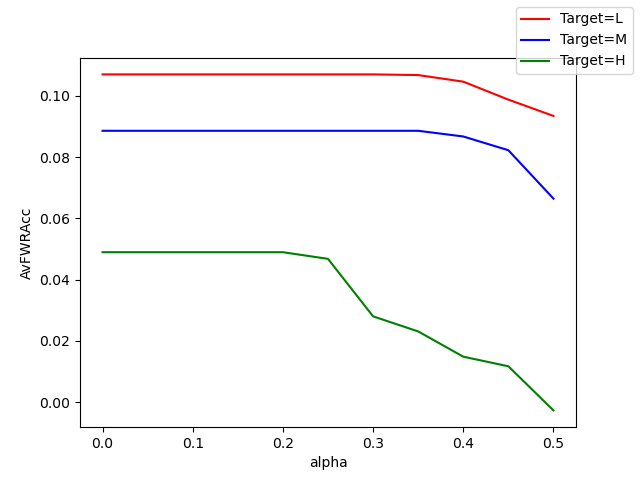
\includegraphics[scale=0.4]{mincov_oe_fwracc.png}
		\caption{$AvFWRAcc$ w.r.t $\alpha$ in SDFIOE.}
	\end{subfigure}\hspace{0.5cm}
	\begin{subfigure}{.4\textwidth}
		\centering
		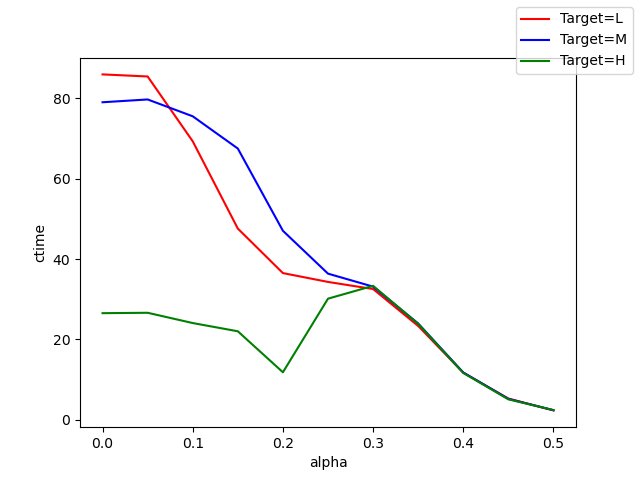
\includegraphics[scale=0.4]{mincov_oe_ctime.png}
		\caption{$Ctime$ w.r.t $\alpha$ in SDFIOE.}
	\end{subfigure}\\
	\begin{subfigure}{.4\textwidth}
		\centering
		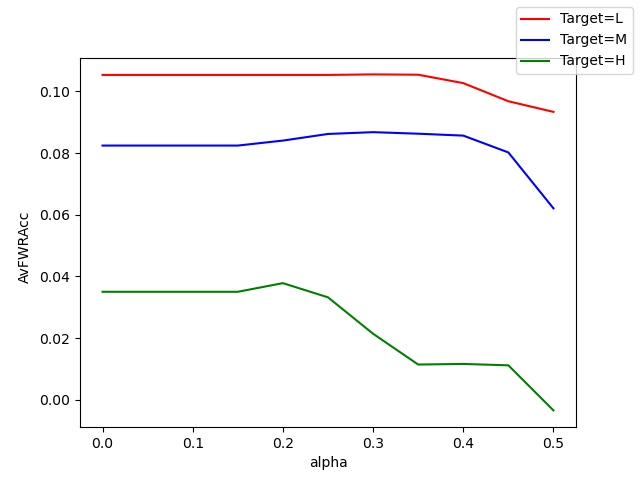
\includegraphics[scale=0.4]{mincov_w_fwracc.png}
		\caption{$AvFWRAcc$ w.r.t $\alpha$ in GSDFIW.}
	\end{subfigure}\hspace{0.5cm}
	\begin{subfigure}{.4\textwidth}
		\centering
		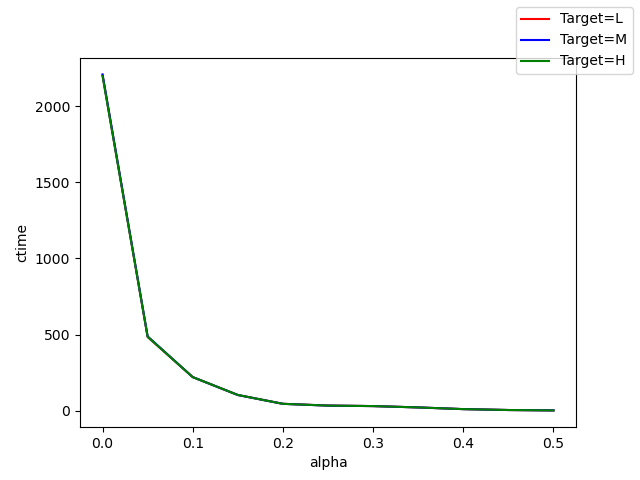
\includegraphics[scale=0.4]{mincov_w_ctime.png}
		\caption{$Ctime$ w.r.t $\alpha$ in GSDFIW.}
	\end{subfigure}
	\caption{Plots of the $AvFWRAcc$ and the computation time in seconds ($Ctime$) with respect to the minimum $FCoverage$ ($\alpha$) obtained when executing the algorithms SDFIOE and GSDFIW for the dataset WPBC, with a uniform fuzzy partition with three fuzzy sets with triangular membership functions for the numeric variables, $I=\IGD$, $T=\TM$, $MaxFeatures =5$, $k=10$ and $\lambda = 0.7$.}
	\label{fig:SD:1}
\end{figure}

 In Plots (a) and (c) of Figure \ref{fig:SD:1}, we can see that in both algorithms the precision on the measure $FWRAcc$ starts to decrease visibly when $\alpha$ is bigger or equal to $0.25$ and the target's label is $H$. For the other two labels this does not happen until $\alpha$ is bigger or equal to $0.35$. With respect to the computation time, we can see that it is reduced when $\alpha$ increases even if we do not lose precision, i.e., even if $\alpha \leq 0.2$. Moreover, it is clear that SDFIOE is faster than GSDFIW, this is due to the fact that in the second algorithm an optimistic pruning technique is not available. However, for values $\alpha \geq 0.1$ the computation time of GSDFIW decreases significantly. It is interesting to point out that in Plot (b) the computation time is not monotone with respect to $\alpha$, this is due to the presence  of the optimistic estimate. Most likely, when we increase $\alpha$ from $0.2$ to $0.25$, the algorithm discards one of the best candidates previously considered, and this negatively affects the computation time. Further, if we compare again Plots (a) and (c), we can notice that the values of $AvFWRAcc$ are lower in GSDFIW than in SDFIOE. Indeed, as we comment later on, the weighted covering algorithm provides sets of output rules with less $AvFWRAcc$ in order to obtain a higher fuzzy overall coverage. 
 
  \begin{figure}[H]
 	\centering
 	\begin{subfigure}{.4\textwidth}
 		\centering
 		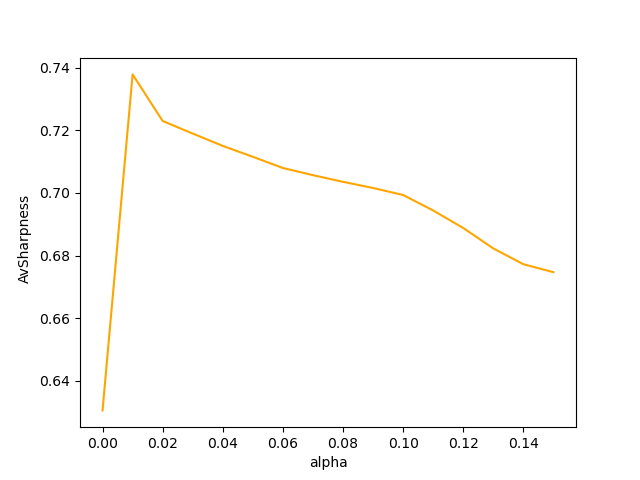
\includegraphics[scale=0.4]{mincov_sharp_sharpness.png}
 		\caption{$AvSharpness$ w.r.t $\alpha$ in STFI.}
 	\end{subfigure}\hspace{0.5cm}
 	\begin{subfigure}{.4\textwidth}
 		\centering
 		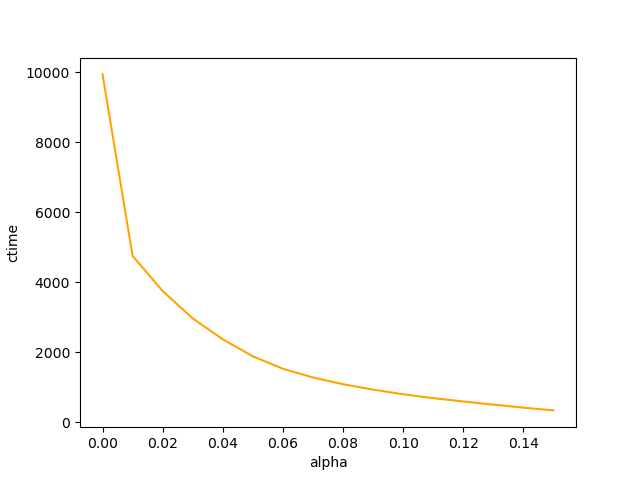
\includegraphics[scale=0.4]{mincov_sharp_ctime.png}
 		\caption{$Ctime$ w.r.t $\alpha$ in STFI.}
 	\end{subfigure}
 	\begin{subfigure}{.4\textwidth}
 		\centering
 		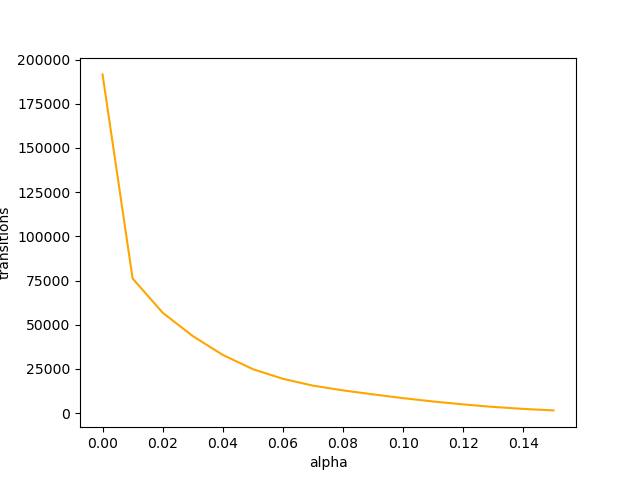
\includegraphics[scale=0.4]{mincov_sharp_ntransitions.png}
 		\caption{$NTransitions$ w.r.t $\alpha$ in STFI.}
 	\end{subfigure}
 	\caption{Plots of the $AvSharpness$, the computation time in seconds ($Ctime$) and the number of transitions ($NTransitions$) with respect to the minimum $FCoverage$ ($\alpha$) obtained when executing the algorithm STFI for the dataset WPBC, with a uniform fuzzy partition with three fuzzy sets with triangular membership functions for the numeric variables, $I=\IGD$, $T=\TM$ and $MaxFeatures =5$.}
 	\label{fig:SD:2}
 \end{figure}
 
 On the other hand, we have performed an analogous study but for the algorithm STFI and $\alpha \in \{0,0.01,0.02,\dots,0.16\}$, obtaining the results in Figure \ref{fig:SD:2}. In this case, we can see that the computation time and the number of transitions obtained decrease with respect to $\alpha$. In fact, for $\alpha \geq 0.17$ the algorithm does not provide any sharp transition, so we can conclude that this algorithm is more sensitive to the parameter $\alpha$ than SDFIOE and GSDFIW. However, the interpretation of these results is rather different than the one of Figure \ref{fig:SD:1}, because in this case we are not optimizing any measure but we are searching for transitions, which are returned ordered in terms of the measure $Sharpness$. Therefore, although the average $Sharpness$ of all the obtained transtions ($AvSharpness$) decreases with respect to $\alpha$, from this fact we can only derive that in each iteration we are discarding the transitions that do not fulfill the minimum required fuzzy coverage. For instance, if we select $\alpha \geq 0.1$, the computation time decreases dramatically but the algorithm still finds plenty of transitions without a drastic drop in $AvSharpness$.
 
In view of these results and similar ones obtained for the other datasets, we think it is reasonable to consider $\alpha=0.1$ in all three algorithms for the rest of the computations of this section. Further on, the algorithms SDFIOE and GSDFIW will be always executed independently for each one of the labels of the target variable. Accordingly, for each label we compute the average $FWRAcc$ of the $k=10$ output rules, which is denoted by $AvFWRAcc$. For the algorithm STFI, the total number of transitions obtained is denoted by $NTransitions$ and the average of the $Sharpness$ of this total is denoted by $AvSharpness$.

% Fuzzy Partition vs Fuzzy Operators
Next, we discuss the behavior of the algorithms with respect to the choice of the fuzzy partitions for the numeric variables and the pair $(I,T)$ of fuzzy implication function $I$ and t-norm $T$. It is recurrent in the literature to affirm that depending on the concrete problem different fuzzy implication functions can be adequate \cite{Trillas2008}. Regarding our problem, in Section \ref{section:pair(I,T)} we have thoroughly discussed from a theoretical point of view which additional properties are recommended for a pair $(I,T)$ in order to behave adequately when used in the subgroup discovery task (see Definition \ref{def:adequate_pair}). However, in this section we want to test the six pairs gathered in Table \ref{table:selectedoperators} from an experimental point of view.  For those pairs in Table \ref{table:selectedoperators} that depend on a parameter, we have selected one arbitrarily. Thus, the selected pairs are:
\begin{equation}\label{eq:six_pairs}
(\IGD,\TM), \quad (\IGG,\TP), \quad (I_{\bm{ FGM(0.5)}},\TP), \quad (I^{\bm{SS}}_{k_{-1}},T_{\bm{-1}}^{\bm{SS}}), \quad (I^{\bm{H}}_{k_2},T_2^{\bm{H}}), \quad  (I^{\bm{F}}_{k_2},T_2^{\bm{F}}).
\end{equation}
Concerning fuzzy partitions, it is well known that the selection and design of the fuzzy sets for the linguistic variables involved in any problem regarding fuzzy modeling affects the interpretability and performance of an algorithm \cite{Cordon2000}. Indeed, the number of linguistic labels (granularity), the shape of the membership functions and the corresponding parameters should be chosen with some assurance that they are suitable for the situation of interest. The ideal situation is when an expert can use his/her knowledge to determine the corresponding membership functions of the fuzzy sets and the linguistic labels for each variable. Unfortunately, this is not usually the case, either the expert is not able to successfully provide the corresponding information or no expert information is available at all. A common way of dealing with this problem is to define uniform fuzzy partitions, in which the fuzzy sets are equally distributed on the range of values, with the same number of linguistic labels (usually three or five) for each one of the numeric variables. Moreover, usually the triangular or trapezoidal type of membership functions are used. However, it has been discussed that the uniform fuzzy partition may not be adequate when the corresponding numeric variable is not uniformly distributed, for instance, in the case when it presents outliers \cite{Li2008,Uriz2020}. To address this situation, different automatic fuzzy partitioning methods have been introduced in the literature \cite{Uriz2020}. Since we do not have expert knowledge available for any of the databases of Table \ref{table:databases}, we have considered some fuzzy partitioning methods which have an available Python implementation. Specifically, apart from the uniform partition, we have considered two other methods which are implemented in the package \textit{pyFTS} \cite{Petronio2019} and are based on the clustering techniques CMeans and FCM \cite{Li2008,Bezdek1981}. However, for simplicity's sake, all three methods have been considered with three linguistic labels for each numeric variable and triangle membership functions.

Having said this, we have evaluated the algorithms SDFIOE and STFI for the seven databases of Table \ref{table:databases} and for each combination of the three considered fuzzy automatic partitioning methods (Uniform, CMeans and FCM) and the pairs $(I,T)$ in Equation (\ref{eq:six_pairs}). The mean and standard deviations of the measures $AvFWRAcc$, $AvSharpness$ and $NTransitions$ can be found in Tables \ref{table:PartvsOp:SDFIOE} and \ref{table:PartvsOp:STFI}, respectively.

\begin{table}[H]
	\centering
	\setlength\tabcolsep{7pt}
	\renewcommand{\arraystretch}{1.75} \large
	\resizebox{\textwidth}{!}{
		\begin{tabular}{|c|c|c|c|c|c|c|}
			\hline
			\diagbox[width=10em]{\textbf{Partition}}{\bm{$(I,T)$}}   & $(\IGD,\TM)$ & $(\IGG,\TP)$ & $(I_{\bm{ FGM(0.5)}},\TP)$ & $(I^{\bm{SS}}_{k_{-1}},T_{\bm{-1}}^{\bm{SS}})$ & $(I^{\bm{H}}_{k_2},T_2^{\bm{H}})$ & $(I^{\bm{F}}_{k_2},T_2^{\bm{F}})$ \\ \hline
			\multicolumn{1}{|c|}{\textbf{Uniform}}  & $0.106~(0.050)$  & $0.096~(0.045)$ & $0.044~(0.019)$ & $0.092~(0.042)$ & $0.073~(0.034)$ & $0.085~(0.037)$ \\ \hline
			\multicolumn{1}{|c|}{\textbf{CMeans}} &    $0.089~(0.046)$        &    $0.080~(0.040)$          &     $0.054~(0.030)$       &      $0.080~(0.041)$      &      $0.069~(0.037)$      & $0.075~(0.039)$  \\ \hline
			\multicolumn{1}{|c|}{\textbf{FCM}}  & $0.078~(0.038)$      &   $0.072~(0.035)$         &     $0.051~(0.027)$       &   $0.072~(0.035)$        &   $0.062~(0.031)$         &      $0.069~(0.034)$   \\ \hline
		\end{tabular}
	}
	\caption{Mean and standard deviation of the $AvFWRAcc$ obtained when executing the algorithm SDFIOE for the seven databases of Table \ref{table:databases} with $k=10$, $MaxFeatures=5$, $\alpha=0.1$ and different options for the fuzzy partitioning method of the numeric variables and the pair $(I,T)$.} \label{table:PartvsOp:SDFIOE}
\end{table}

\begin{table}[H]
	\centering
	\setlength\tabcolsep{7pt}
	\renewcommand{\arraystretch}{1.75} \large
	\subfloat[$AvSharpness$.]{
		\resizebox{\textwidth}{!}{
			\begin{tabular}{|c|c|c|c|c|c|c|}
				\hline
				\diagbox[width=10em]{\textbf{Partition}}{\bm{$(I,T)$}}   & $(\IGD,\TM)$ & $(\IGG,\TP)$ & $(I_{\bm{ FGM(0.5)}},\TP)$ & $(I^{\bm{SS}}_{k_{-1}},T_{\bm{-1}}^{\bm{SS}})$ & $(I^{\bm{H}}_{k_2},T_2^{\bm{H}})$ & $(I^{\bm{F}}_{k_2},T_2^{\bm{F}})$ \\ \hline
				\multicolumn{1}{|c|}{\textbf{Uniform}} & \multicolumn{1}{c|}{$0.800~(0.068)$}&  \multicolumn{1}{c|}{$0.766~(0.056)$}                & \multicolumn{1}{c|}{$0.560~( 0.052)$}                & \multicolumn{1}{c|}{$0.773~(0.070)$}                & \multicolumn{1}{c|}{$0.681~(0.041)$} & $0.725~(0.048)$                \\ \hline
				\multicolumn{1}{|c|}{\textbf{CMeans}}  & \multicolumn{1}{c|}{$0.585~(0.077)$}                & \multicolumn{1}{c|}{$0.570~(0.057)$}                & \multicolumn{1}{c|}{$0.480~( 0.051)$}                & \multicolumn{1}{c|}{$0.561~(0.061)$}                & \multicolumn{1}{c|}{$0.534~(0.048)$} & $0.553~(0.056)$                \\ \hline
				\multicolumn{1}{|c|}{\textbf{FCM}}     & \multicolumn{1}{c|}{$0.568~(0.098)$}& \multicolumn{1}{c|}{$0.57~(0.119)$}                & \multicolumn{1}{c|}{$0.490~( 0.132)$}                & \multicolumn{1}{c|}{$0.571~( 0.125)$}                & \multicolumn{1}{c|}{$0.539~(0.140)$} & $0.556~(0.128)$                 \\ \hline
			\end{tabular}
		}
	}
	\\
	\vspace{0.5cm}
	\subfloat[$NTransitions$.]{
		\resizebox{\textwidth}{!}{
			\begin{tabular}{|c|c|c|c|c|c|c|}
				\hline
				\diagbox[width=10em]{\textbf{Partition}}{\bm{$(I,T)$}}   & $(\IGD,\TM)$ & $(\IGG,\TP)$ & $(I_{\bm{ FGM(0.5)}},\TP)$ & $(I^{\bm{SS}}_{k_{-1}},T_{\bm{-1}}^{\bm{SS}})$ & $(I^{\bm{H}}_{k_2},T_2^{\bm{H}})$ & $(I^{\bm{F}}_{k_2},T_2^{\bm{F}})$ \\ \hline
				\multicolumn{1}{|c|}{\textbf{Uniform}} & \multicolumn{1}{c|}{$5322.000~(8583.921)$}                & \multicolumn{1}{c|}{$299.857~(328.371)$}                & \multicolumn{1}{c|}{$175.286~( 227.521)$}                & \multicolumn{1}{c|}{$1519.429~(2838.679)$}                & \multicolumn{1}{c|}{$150.286~(155.788)$}&  $211.00~(228.141)$               \\ \hline
				\multicolumn{1}{|c|}{\textbf{CMeans}}  & \multicolumn{1}{c|}{$1237.000~(1962.839)$}                & \multicolumn{1}{c|}{$164.286~(202.562)$} & \multicolumn{1}{c|}{$162.143~( 200.678)$}                & \multicolumn{1}{c|}{$369.429~(533.136)$}                & \multicolumn{1}{c|}{$116.857~(137.964)$} &  $144.000~(178.273)$               \\ \hline
				\multicolumn{1}{|c|}{\textbf{FCM}}     & \multicolumn{1}{c|}{$339.429~(350.002)$}                & \multicolumn{1}{c|}{$95.000~(89.413)$}    & \multicolumn{1}{c|}{$88.143~(88.209)$}                & \multicolumn{1}{c|}{$148.429~(143.824)$}                & \multicolumn{1}{c|}{$75.714~( 79.785)$}                &         $87.000~(83.968)$        \\ \hline
			\end{tabular}
		}
	}
	
	\caption{Mean and standard deviation of $AvSharpness$ and $NTransitions$ obtained when executing the algorithm STFI for the seven databases of Table \ref{table:databases} with $MaxFeatures=5$, $\alpha=0.1$ and different options for the fuzzy partitioning method of the numeric variables and the pair $(I,T)$.} \label{table:PartvsOp:STFI}
\end{table}

From the information gathered in Tables \ref{table:PartvsOp:SDFIOE} and \ref{table:PartvsOp:STFI} we can clearly see that the choice of the fuzzy partition and the pair $(I,T)$ significantly affects the value of the quantities $AvFWRAcc$, $AvSharpness$ and $NTransitions$. For instance, in Table \ref{table:PartvsOp:SDFIOE} the pair  $(I_{\bm{ FGM(0.5)}},\TP)$ provides lower values of $AvFWRAcc$ than other pairs. Besides, for a fixed pair $(I,T)$, the uniform partition generally obtains higher values of $AvFWRAcc$ in comparison with the other two fuzzy partitioning methods. Moreover, the selection of  a uniform partition and $(\IGD,\TM)$ provides the highest mean of $AvFWRAcc$ and $AvSharpness$. Nonetheless, from these results we cannot conclude that any of these combinations is better than another. Let us stress that all the measures introduced in Section \ref{subsection:quality_measures} are defined in terms of the pair $(I,T)$ and they are evaluated recalling the membership functions of the corresponding fuzzy sets. Therefore, it is not adequate to compare any of these measures when different fuzzy partitions or pairs $(I,T)$ are considered. Not only from Tables \ref{table:PartvsOp:SDFIOE} and \ref{table:PartvsOp:STFI} we cannot conclude which combination is the best, but we cannot even claim that the corresponding subgroups sets are significantly different between any of these cases. Indeed, an IF-THEN fuzzy rule modeled by different pairs $(I,T)$ or evaluated in distinct fuzzy partitions will have different values of the considered measures. Let us point out again that the ultimate goal of these algorithms is the interpretation of the output as IF-THEN rules, so we are actually more interested in knowing if the contemplated cases provide sets of output rules with different linguistic IF-THEN representation. With respect to this topic, in Panel (b) of Table \ref{table:PartvsOp:STFI} we can notice that the number of transitions discovered by STFI is very different depending on the case. Indeed, the FCM partition tends to output less sharp transitions than the other two fuzzy partitioning methods. On the other hand, to quantify the similarity between two sets of fuzzy rules obtained by the algorithm SDFIOE we will consider that two rules are equivalent if they are constructed with the exact same pairs of (feature,linguistic label). From a theoretical point of view, this might seem strange, because if we have considered different fuzzy operators and fuzzy partitions, two fuzzy rules are not equal even if their linguistic representation as IF-THEN rules look the same. Indeed, although we use the same linguistic labels for two fuzzy partitions of the same numeric variable, the meaning of these labels is distinct. Nonetheless, we think that it is interesting to study if sets of subgroups given as IF-THEN rules look similar because this representation is a key element in the interpretation of the results. Having said this, to compare two sets of fuzzy rules we have considered the Jaccard similarity index \cite{Tan2018}. Specifically, if $SR_1 = \{R_{1,1},\dots,R_{1,k}\}$ and $SR_2=\{R_{2,1},\dots,R_{2,k}\}$ are two sets of fuzzy rules, we define the percentage of similarity as
$$ Similarity(SR_1,SR_2)=\frac{|SR_1 \cap SR_2|}{|SR_1 \cup SR_2|} \cdot 100,$$
where we have considered that $R_{1,l} = R_{2,\tilde{l}}$ if they involve the same target class and the same linguistic labels of the feature variables. In accordance, if we want to compare different fuzzy partitioning methods we have to consider the same granularity and the same linguistic labels for each numeric variable.

Having said this, we have computed the mean of the percentage of similarity between the set of rules obtained for a fixed target class when we execute the algorithm SDFIOE for the seven databases of Table \ref{table:databases}, the Uniform and FCM fuzzy partitioning methods and the six pairs $(I,T)$ in Equation (\ref{eq:six_pairs}). Specifically, in Table \ref{table:UniformvsFCM} we have compared the results obtained with the Uniform and FCM partitioning methods and in Table \ref{table:FCMvsFCM} we study the scenario when the FCM method is fixed and we only variate the pair $(I,T)$. From the results in Table \ref{table:UniformvsFCM} we can clearly see that modifying the fuzzy partitioning method drastically changes the obtained subgroups even if we use the same pair $(I,T)$. Therefore, we can conclude that the design of the corresponding fuzzy partition of the numeric variables is a very important step for the posterior interpretation of the fuzzy rules. Indeed, it is clear that if this step is downplayed it is very hard to interpret why changing the fuzzy partitioning method results in a completely different set of subgroups represented as IF-THEN rules. Nonetheless, in this report we do not have expert knowledge for any of the databases of Table \ref{table:databases}. Therefore, for the rest of experiments we think that the FCM partitioning method is the most adequate of the three considered, because it is more robust and since its meaning is linked to the corresponding fuzzy clustering technique. On the other hand, in Table \ref{table:FCMvsFCM} we can see that only modifying the pair $(I,T)$ does not cause such a drastic change, although the results are also significantly different depending on the selected fuzzy operators. In this case, the choice of the pair $(I,T)$ represents how are we mathematically interpreting the logical conditional in the corresponding subgroups. After all, if we change the pair $(I,T)$ we are studying different ways in which the target variable may be related to the considered features. In this sense, our algorithm is very versatile, because if for a certain configuration the output does not disclose new or relevant information, for another pair of operators the obtained rules may capture different relations from the mathematical point of view. However, a deeper study is needed to properly interpret the meaning behind the use of different pairs $(I,T)$.

%Moreover, we will further discuss the selection $(I,T)$ with respect to the weighted covering algorithm.
%Nonetheless, in this case is more hard to justify which pair $(I,T)$ will be adequate in each case.
%Moreover, we will further discuss the selection $(I,T)$ with respect to the weighted covering algorithm.

\begin{table}[ht!]
	\centering
	\setlength\tabcolsep{7pt}
	\renewcommand{\arraystretch}{1.75} \large
	\resizebox{12cm}{!}{
		\begin{tabular}{|c|c|c|c|c|c|c|}
			\hline
			\diagbox[width=11em]{\textbf{Uniform},~$(I,T)$}{\textbf{FCM},~$(I,T)$} & $(\IGD,\TM)$ & $(\IGG,\TP)$ & $(I_{\bm{ FGM(0.5)}},\TP)$ & $(I^{\bm{SS}}_{k_{-1}},T_{\bm{-1}}^{\bm{SS}})$ & $(I^{\bm{H}}_{k_2},T_2^{\bm{H}})$ & $(I^{\bm{F}}_{k_2},T_2^{\bm{F}})$ \\ \hline
			\multicolumn{1}{|c|}{$(\IGD,\TM)$} & 10.492\%    &  9.604\%     &  9.859\%      &  11.953\%      & 9.254\%    &  9.676\%     \\ \hline
			\multicolumn{1}{|c|}{$(\IGG,\TP)$} &    8.975\%    & 11.038\%      & 11.435\%     & 10.727\%      &   11.435\%    & 11.388\%     \\ \hline
			\multicolumn{1}{|c|}{$(I_{\bm{ FGM(0.5)}},\TP)$} &    9.651\%    &  11.106\%      &   14.923\%   &  11.456\%     &  11.806\%    &   11.456\%    \\ \hline
			\multicolumn{1}{|c|}{$(I^{\bm{SS}}_{k_{-1}},T_{\bm{-1}}^{\bm{SS}})$} &    9.778\%    &  10.661\%   & 10.927\%        &  11.362\%   &  10.661\%    &   10.700\%    \\ \hline
			\multicolumn{1}{|c|}{$(I^{\bm{H}}_{k_2},T_2^{\bm{H}})$} &   9.046\%     &    10.190\%    &  11.439\%      &    10.851\%    & 10.898\%     & 10.540\%     \\ \hline
			\multicolumn{1}{|c|}{$(I^{\bm{F}}_{k_2},T_2^{\bm{F}})$} &    9.325\%    &   11.005\%     &    11.052\%    &    11.044\%    &     11.402\%   & 11.356\%       \\ \hline
		\end{tabular}
	}
	\caption{Mean of the percentage of similarity between the list of rules obtained  when executing the algorithm SDFIOE for the seven databases of Table \ref{table:databases} with $k=10$, $MaxFeatures=5$, $\alpha=0.1$ and different options for the fuzzy partitioning method of the numeric variables and the pair $(I,T)$.}\label{table:UniformvsFCM}
\end{table}

\begin{table}[ht!]
	\centering
	\setlength\tabcolsep{7pt}
	\renewcommand{\arraystretch}{1.75} \large
	\resizebox{12cm}{!}{
		\begin{tabular}{|c|c|c|c|c|c|c|}
			\hline
			{\diagbox[width=11em]{\textbf{FCM},~$(I,T)$}{\textbf{FCM},~$(I,T)$}} & $(\IGD,\TM)$ & $(\IGG,\TP)$ & $(I_{\bm{ FGM(0.5)}},\TP)$ & $(I^{\bm{SS}}_{k_{-1}},T_{\bm{-1}}^{\bm{SS}})$ & $(I^{\bm{H}}_{k_2},T_2^{\bm{H}})$ & $(I^{\bm{F}}_{k_2},T_2^{\bm{F}})$ \\ \hline
			\multicolumn{1}{|c|}{$(\IGD,\TM)$} & 100.000\%    &  61.728\%     &  54.044\%      &  74.798\%      & 57.322\%    &  60.577\%     \\ \hline
			\multicolumn{1}{|c|}{$(\IGG,\TP)$} &    61.728\%    & 100.000\%      &  69.239\%     &  78.742\%      &    81.208\%    & 91.486\%     \\ \hline
			\multicolumn{1}{|c|}{$(I_{\bm{ FGM(0.5)}},\TP)$} &    54.044\%    &  69.239\%      &   100.000\%   &  66.541\%     &   73.171\%    &   72.624\%    \\ \hline
			\multicolumn{1}{|c|}{$(I^{\bm{SS}}_{k_{-1}},T_{\bm{-1}}^{\bm{SS}})$} &    74.798\%    &  78.742\%   & 66.541\%        &   100.000\%   &  71.798\%    &    78.487\%    \\ \hline
			\multicolumn{1}{|c|}{$(I^{\bm{H}}_{k_2},T_2^{\bm{H}})$} &   57.322\%     &    81.208\%    &  73.171\%      &   71.798\%    &    100.000\%     &    84.271\%     \\ \hline
			\multicolumn{1}{|c|}{$(I^{\bm{F}}_{k_2},T_2^{\bm{F}})$} &    60.577\%    &   91.486\%     &    72.624\%    &    78.487\%    &     84.271\%   &  100.000\%       \\ \hline
		\end{tabular}
	}
	\caption{Mean of the percentage of similarity between the list of rules obtained  when executing the algorithm SDFIOE for the seven databases of Table \ref{table:databases} with $k=10$, $MaxFeatures=5$, $\alpha=0.1$, a FCM partition and different options for the pair $(I,T)$.}\label{table:FCMvsFCM}
\end{table}

% Lambdas vs Fuzzy Operators
Further, we discuss the performance of the considered pairs $(I,T)$ with respect to the weighted covering algorithm designed in Section \ref{section:SDalgorithms} based on Equation (\ref{eq:example_weights_concrete}).  Let us recall that for the fuzzy negation we are using the Sugeno class $N^{\lambda}$ which depends on the parameter $\lambda \in (-\infty,1)$ and for the t-conorm we are using the $N^{\lambda}$-dual of the corresponding t-norm. Thus, the weighted covering algorithm and the computation of the fuzzy overall coverage depend on the value of $\lambda$. For the study of the weighted covering algorithm with respect to the parameter $\lambda$ and the selection of the pair $(I,T)$ we have two options: to consider the exact algorithm GSDFIW or to use the post-processing technique WCSDFI that can be combined with SDFIOE. Since GSDFIW is significantly more computationally expensive than SDFIOE, we have opted for using the second perspective for this section. In order to combine the two algorithms, the schema considered is to first execute SDFIOE to obtain $1000$ rules and then use WCSDFI to select only a 1\% of these rules, i.e., to obtain 10 final rules. This way, if we want to evaluate different values of $\lambda$ we only have to rerun the post-processing technique WCSDFI. To simplify, we denote this schema by SDFIOE+WCSDFI with $(\tilde{k},k)=(1000,10)$ and $\lambda \in (+\infty,1)$. From this procedure, we aim to obtain sets of output rules with a higher fuzzy overall coverage ($OvFCoverage$) than the results obtained when executing only  SDFIOE with $k=10$. In order to compare the loss of precision on $AvFWRAcc$ and the gain of $OvFCoverage$ we have considered the relative change \cite{Tornqvist1985}. The relative change is a measure that quantifies the change of a value $x$ with respect to a reference value $x_{ref}$, and it is defined as follows:
$$RC(x,x_{ref}) = \frac{x-x_{ref}}{x_{ref}}.$$
One of the most remarkable characteristics of this quantity is that its value is independent of the unit of measurement employed. In our case, we aim to compare the change of the measures $AvFWRAcc$ and $OvFCoverage$ of the 10 output rules obtained when executing SDFIOE+WCSDFI with $(\tilde{k},k)=(1000,10)$ and $\lambda \in (+\infty,1)$ in reference to only using SDFIOE with $k=10$.  Thus, we consider the following quantities:
\begin{itemize}
	\item $AvFWRAcc_1$ as the $AvFWRAcc$ of the $10$ rules obtained for  a certain target class when executing SDFIOE with $k=10$.
	\item $OvFCoverage_{1,\lambda}$ as the $OvCoverage$ computed with $\lambda \in (-\infty,1)$ and the 10 rules obtained for a certain target class when executing SDFIOE with $k=10$ .
	\item $AvFWRAcc_{2,\lambda}$ as the $AvFWRAcc$ of the $10$ rules obtained for  a certain target class when executing SDFIOE+WCSDFI with $(\tilde{k},k)=(1000,10)$ and $\lambda \in (+\infty,1)$.
	\item $OvFCoverage_{2,\lambda}$ as the $OvCoverage$ computed with $\lambda \in (-\infty,1)$ and the 10 rules obtained for a certain target class when executing SDFIOE+WCSDFI with $(\tilde{k},k)=(1000,10)$ and the same $\lambda$.
\end{itemize}
In accordance, we define the relative change of the measures $AvFWRAcc$ and $OvFCoverage$ as follows:
\begin{eqnarray*}
	\frac{\Delta AvFWRAcc}{AvFWRAcc_1} &=& \frac{AvFWRAcc_{2,\lambda} - AvFWRAcc_1}{AvFWRAcc_1}, \\
	\frac{\Delta OvCoverage}{OvCoverage_{1,\lambda}} &=& \frac{OvCoverage_{2,\lambda}-OvCoverage_{1,\lambda}}{OvCoverage_{1,\lambda}}.
\end{eqnarray*}

Having said this, we have computed the average relative change for each target class of the seven databases in Table \ref{table:databases} and the six pairs $(I,T)$ in Equation (\ref{eq:six_pairs}) for $\lambda \in \{0.25,0.5,0.75,0.9\}$. The results can be found in Table \ref{table:lambdas}. From this outcome we can clearly see that for all the selected pairs $(I,T)$, generally if we decrease the value of $\lambda$ then the $OvFCoverage$ increases and the $AvFWRAcc$ decreases. Therefore, we can conclude that the implemented weighted covering algorithm has the desired behavior. Further, in the subsequent section (see Section \ref{subsection:acasestudy}) we show for a concrete case that the growth of the $OvFCoverage$ is also noticeable when interpreting the subgroups in the form of IF-THEN rules. Since the design of this schema is based on a generalization of a crisp concept to fuzzy logic, it is very positive to disclose that it has the required effect. Therefore, apart from being a very intuitive algorithm, we have seen that it is also effective. On the other hand, the selection of the pair $(I,T)$ also affects the performance of the weighted covering algorithm. For instance, for the pair $(\IGD,\TM)$ we lose less precision on $AvFWRAcc$ but also the improvement on the $OvFCoverage$ is not that pronounced. This behavior is intuitive, because if we consider Equation (\ref{eq:example_weights_concrete}) with the minimum t-norm we can notice that, when we incorporate a new rule in an iteration, the example's weights may not be modified. Indeed, the minimum does not have an accumulative behavior in the weighted covering algorithm. On the other hand, the pairs $(\IGG,\TP)$ and $(I^{\bm{F}}_{k_2},T_2^{\bm{F}})$ provide a good balance between the improvement of the $OvFCoverage$ and the loss of $AvFWRAcc$. This resemblance may be related to Table \ref{table:FCMvsFCM}, since these two pairs are the most similar with respect to the set of output rules when executing SDFIOE.


%To sum up, we can conclude that the pair of operators $(I,T)$ can be modified for two purposes:
%\begin{itemize}
%	\item To obtain different IF-THEN rules, that will capture different relations between the features and the target variables.
%		\item To obtain the desired behavior
%	\end{itemize}

\begin{table}[ht]
	\centering
	\setlength\tabcolsep{7pt}
	\renewcommand{\arraystretch}{1.75} \large
	\subfloat[$\frac{\Delta AvFWRAcc}{AvFWRAcc_1}$.]{
		\resizebox{10cm}{!}{
			\begin{tabular}{|c|c|c|c|c|c|c|}
	\hline
	\diagbox[width=5em]{\textbf{$\lambda$}}{$(I,T)$}   & $(\IGD,\TM)$ & $(\IGG,\TP)$ & $(I_{\bm{ FGM(0.5)}},\TP)$ & $(I^{\bm{SS}}_{k_{-1}},T_{\bm{-1}}^{\bm{SS}})$ & $(I^{\bm{H}}_{k_2},T_2^{\bm{H}})$ & $(I^{\bm{F}}_{k_2},T_2^{\bm{F}})$ \\ \hline
	\multicolumn{1}{|c|}{$0.25$} & \multicolumn{1}{c|}{$-0.088$}                & \multicolumn{1}{c|}{$-0.245$}                & \multicolumn{1}{c|}{$-0.330$}                & \multicolumn{1}{c|}{$-0.151$}                & \multicolumn{1}{c|}{$-0.325$}&  $-0.269$               \\ \hline
	\multicolumn{1}{|c|}{0.5}  & \multicolumn{1}{c|}{$-0.082$}                & \multicolumn{1}{c|}{$-0.229$} & \multicolumn{1}{c|}{$-0.298$}                & \multicolumn{1}{c|}{$-0.127$}                & \multicolumn{1}{c|}{$-0.292$} &  $-0.255$               \\ \hline
	\multicolumn{1}{|c|}{0.75}     & \multicolumn{1}{c|}{$-0.050$}                & \multicolumn{1}{c|}{$-0.183$}    & \multicolumn{1}{c|}{$-0.243$}                & \multicolumn{1}{c|}{$-0.099$}                & \multicolumn{1}{c|}{$-0.250$}                &         $-0.200$        \\ \hline
	\multicolumn{1}{|c|}{0.9}     & \multicolumn{1}{c|}{$-0.034$}                & \multicolumn{1}{c|}{$-0.121$}    & \multicolumn{1}{c|}{$-0.177$}                & \multicolumn{1}{c|}{$-0.056$}                & \multicolumn{1}{c|}{$-0.178$}                &         $-0.140$        \\ \hline
\end{tabular}
		}
	}
	\\
	\vspace{0.5cm}
	\subfloat[$\frac{\Delta OvFCoverage}{OvFCoverage_{1,\lambda}}$.]{
		\resizebox{10cm}{!}{
			\begin{tabular}{|c|c|c|c|c|c|c|}
				\hline
				\diagbox[width=5em]{\textbf{$\lambda$}}{$(I,T)$}   & $(\IGD,\TM)$ & $(\IGG,\TP)$ & $(I_{\bm{ FGM(0.5)}},\TP)$ & $(I^{\bm{SS}}_{k_{-1}},T_{\bm{-1}}^{\bm{SS}})$ & $(I^{\bm{H}}_{k_2},T_2^{\bm{H}})$ & $(I^{\bm{F}}_{k_2},T_2^{\bm{F}})$ \\ \hline
				\multicolumn{1}{|c|}{0.25} & \multicolumn{1}{c|}{$0.115$}                & \multicolumn{1}{c|}{$0.215$}                & \multicolumn{1}{c|}{$0.263$}                & \multicolumn{1}{c|}{$0.132$}                & \multicolumn{1}{c|}{$0.259$}&  $0.246$               \\ \hline
				\multicolumn{1}{|c|}{0.5}  & \multicolumn{1}{c|}{$0.115$}                & \multicolumn{1}{c|}{$0.222$} & \multicolumn{1}{c|}{$0.254$}                & \multicolumn{1}{c|}{$0.135$}                & \multicolumn{1}{c|}{$0.253$} &  $0.236$               \\ \hline
				\multicolumn{1}{|c|}{0.75}     & \multicolumn{1}{c|}{$0.033$}                & \multicolumn{1}{c|}{$0.207$}    & \multicolumn{1}{c|}{$0.227$}                & \multicolumn{1}{c|}{$0.135$}                & \multicolumn{1}{c|}{$0.238$}                &         $0.224$        \\ \hline
								\multicolumn{1}{|c|}{0.9}     & \multicolumn{1}{c|}{$-0.004$}                & \multicolumn{1}{c|}{$0.172$}    & \multicolumn{1}{c|}{$0.183$}                & \multicolumn{1}{c|}{$0.104$}                & \multicolumn{1}{c|}{$0.230$}                &         $0.194$        \\ \hline
			\end{tabular}
		}
	}
	
	\caption{Mean of the relative change between the measures $AvFWRAcc$ and $OvCoverage$ obtained at executing SDFIOE+WCSDFI with $(\tilde{k},k)=(1000,10)$ and $\lambda \in \{0.25,0.5,0.75,0.9\}$ with respect to only executing SDFIOE with $k=10$ for the seven databases of Table \ref{table:databases}. In both situations, the selected parameters for SDFIOE have been $MaxFeatures=5$, $\alpha=0.1$ and a FCM partition for the numeric variables.}\label{table:lambdas}
\end{table}

\newpage

To end this section we want to add a brief comment regarding the computational efficiency of our algorithms. As we have repeatedly stated, our approach in this chapter has been providing simple exhaustive algorithms instead of focusing on efficiency. This has enabled us to perform a thorough study regarding the selection of the algorithm's parameters for the small datasets of Table \ref{table:databases} without the inaccuracy of a search heuristic. Nonetheless, to exemplify the computational cost of the experiments conducted in this section we have displayed in Figure \ref{fig:SD:computation_times} the computation time of executing the schema SDFIOE+WCSDFI and the algorithm STFI for the seven datasets in Table \ref{table:databases} in the following scenario: $MaxFeatures=5$, $\alpha=0.1$, $I=\IGG$, $T=\TP$, FCM partitioning method with three linguistic labels for the numeric variables, $(\tilde{k},k)=(1000,10)$ and $\lambda=0.85$. From these results we can conclude that our algorithms can manage small datasets without any difficulties. Nonetheless, for the dataset ``California Housing'' the total cost of executing SDFIOE+WCSDFI for the three target classes and the algorithm STFI is approximately of 2.5 hours. Therefore, it is clear that the computation time escalates rapidly with respect to the number of instances and the considered features. Thus, a search heuristic should be implemented for our algorithms to be suitable for large datasets.
\pgfplotstableread{
	Label SDFIOE1 SDFIOE2 SDFIOE3 STFI topper
	WPBC 16.367  16.603 16.627 22.26 0.001
	USA2012 44.342  44.766 43.997 74.48 0.001
	Startups 0.502 0.513 0.514 0.54 0.001
	Electricity 6.588 6.641 6.707 11.67 0.001
	StockPrices 115.310 111.840 112.267 259.94 0.001
	Treasury 1000.328 989.003 984.614 2869.63 0.001
	CalHousing 1771.762 1766.394 1759.635 3892.54 0.001
}\testdata


\begin{figure}[ht]
	\centering
	\begin{subfigure}{.4\textwidth}
		\centering
		\begin{tikzpicture}[scale=0.53]
			\begin{axis}[
				ybar stacked,
				x=1.25cm, 
				ymin=0,
				ymax=6000,
				xtick=data,
				legend style={cells={anchor=west}, legend pos=north west},
				reverse legend=false, % set to false to get correct display, but I'd like to have this true
				xticklabels from table={\testdata}{Label},
				xticklabel style={text width=2cm,align=center,rotate=90,font=\footnotesize},
				]
				\addplot [fill=red!80] table [y=SDFIOE1, meta=Label, x expr=\coordindex] {\testdata};
				\addlegendentry{Target=L}
				\addplot [fill=blue!60] table [y=SDFIOE2, meta=Label, x expr=\coordindex] {\testdata};
				\addlegendentry{Target=M}
				\addplot [fill=green!60] table [y=SDFIOE3, meta=Label, x expr=\coordindex] {\testdata};
				\addlegendentry{Target=H}
				\addplot [nodes near coords,point meta=y,nodes near coords style={anchor=south}] table [y=topper, meta=Label, x expr=\coordindex] {\testdata};
			\end{axis}
		\end{tikzpicture}
		\caption{SDFIOE+WCSDFI.}
	\end{subfigure}\hspace{0.5cm}
	\begin{subfigure}{.4\textwidth}
		\centering
		\begin{tikzpicture}[scale=0.53]
			\begin{axis}[
				ybar stacked,
				x=1.25cm, 
				ymin=0,
				ymax=6000,
				xtick=data,
				legend style={cells={anchor=west}, legend pos=north west},
				reverse legend=false, % set to false to get correct display, but I'd like to have this true
				xticklabels from table={\testdata}{Label},
				xticklabel style={text width=2cm,align=center,rotate=90,font=\footnotesize},
				]
				\addplot [fill=orange!80] table [y=STFI, meta=Label, x expr=\coordindex] {\testdata};
				%\addlegendentry{STFI}
				\addplot [nodes near coords,point meta=y,nodes near coords style={anchor=south}] table [y=topper, meta=Label, x expr=\coordindex] {\testdata};
			\end{axis}
		\end{tikzpicture}
		\caption{STFI.}
	\end{subfigure}
	\caption{Plots of the computation time in seconds obtained when executing SDFIOE+WCSDFI and STFI, with a FCM partition for the numeric variables, $I=\IGG$, $T=\TP$, $\alpha=0.1$, $MaxFeatures =5$, $(\tilde{k},k)=(1000,10)$ and $\lambda = 0.85$ for the seven databases of Table \ref{table:databases}.}
	\label{fig:SD:computation_times}
\end{figure}

\newpage

\subsection{A case study: The United States Elections}\label{subsection:acasestudy}

In this section, the algorithms for subgroup discovery based on fuzzy implication functions which have been developed and discussed in this chapter will be applied to a particular problem related to the United States (U.S.) Elections. 

U.S. Elections present some particular features which make them different to the presidential elections of other countries \cite{usagov}. First of all, there are only two political parties: the Republican Party and the Democratic Party. Although independent candidates can also exist, they are rarely elected. Secondly, elections for president of the United States take place every four years on the first Tuesday after the first Monday in November.  U.S. citizens by casting their votes elect members of the ``Electoral College''. This legal body was created by the U.S. Constitution in order to have a system that balances the interests not only of the American people, but also those of the states that conform the Union. It is the Electoral College who elects the president and the vice president of the United States. 

There are 50 states in the United States and each one has a number of electors in the Electoral College equal to the number of its members in the House of Representatives plus the two senators that each state has assigned. The number of members in the House of Representatives per state is computed according to the census of the state's population and the Huntington-Hill apportionment system (also called the method of equal proportions) \cite{censusgovApp}. In addition to the 50 states, the District of Columbia has also three Electoral College votes. This sums up to 538 electors in the Electoral College and therefore, 270 electoral votes are needed to win the presidential election. 

In the United States, one presidential candidate can win the election without obtaining the majority of the votes nationally. The reason underlying this fact is that most states use the winner-take-all system, i.e., the presidential candidate who obtains the highest number of votes in that state receives all the state's electoral votes. There are two exceptions, the states of Nebraska and Maine, which award proportionately some of the electoral votes of the state. Therefore, since it is more important to win in an adequate combination of states than winning the majority of votes nationally, the presidential candidates usually campaign in the so-called competitive or swing states, those needed for their candidacies to reach the 270 electoral votes and where their win is not secure.

Some political analysts state that social and economic factors of the voter are decisive in order to make the final decision on which candidate to vote for (see \cite{economist}). Indeed, there are some religious, economic or racial groups who overwhelmingly vote for the candidate of the Republican or the Democratic Parties, regardless of the personal and political features of the candidate. Consequently, those states with a strong presence of affine groups tend to be favorable for a party. Knowing in advance the social and economic composition of each state and the commitment of each group to each party is greatly helpful for the campaign. 

Focusing on this topic, in this section we will use a dataset that was presented in \cite{Rotger2016}, where a forecast for the 2016 U.S. Elections was proposed by using a generalized linear model regression. The dataset contains variables related to education, religion, race, economy, etc., for the 50 states and the District of Columbia corresponding to 2012. Specifically, the variables and their description are collected in Table \ref{table:usa_features}.

\begin{table}[t]
	\centering
	\setlength\tabcolsep{7pt}
	\renewcommand{\arraystretch}{1.75} \large
	\resizebox{10.5cm}{!}{
	\begin{tabular}{|c|l|}
		\hline
		\textbf{Name}             & \textbf{Description}       \\ \hline
		\textbf{State}            & Name of the state \\ \hline
		%\textbf{Region}           &                            \\ \hline
		\textbf{Density}          & Density of population \\ \hline
		\textbf{Veterans}         & Percentage of veterans, i.e., people who have served in the armed forces \\ \hline
		\textbf{Women}           & Percentage of women \\ \hline
		\textbf{HighSchool\_Grad} & Percentage of high school graduates \\ \hline
		\textbf{University\_Grad} & Percentage of university graduates \\ \hline
		\textbf{Blacks}           & Percentage of people who identify their race as Black\\ \hline
		\textbf{Asians}           & Percentage of people who identify their race as Asian \\ \hline
		\textbf{Hispanics}         & Percentage of people who identify their race as Hispanic or Latino \\ \hline
		\textbf{White}            & Percentage of people who identify their race as White    \\ \hline
		\textbf{Evangelicals}     & Percentage of people who identify their religion as Evangelism  \\ \hline
		\textbf{Protestants}      & Percentage of people who identify their religion as non-evangelical Protestantism \\ \hline
		\textbf{Relig\_Afro}      & Percentage of people who identify their religion as Afro-American \\ \hline
		\textbf{Catholics}        & Percentage of people who identify their religion as Catholicism \\ \hline
		\textbf{Mormons}          & Percentage of people who identify their religion as Mormonism \\ \hline
		\textbf{Retired}          & Percentage of retired people \\ \hline
		\textbf{Unemployment}     & Percentage of unemployed people \\ \hline
		\textbf{Salary}           & Median average annual household income  \\ \hline
		\textbf{Voters}           &  Percentage of votes to the Democratic Party in the 2012 U.S. elections  \\ \hline
	\end{tabular}
}
\caption{Name and description of the variables in the dataset USA2012.}\label{table:usa_features}
\end{table}

The objective of this section is to show the applicability of the algorithms presented in this chapter to this real-life data. Although we are not experts on this topic, we have tried as much as possible to validate our comments with available information provided by analysts of the U.S. elections. Besides, the results will be compared with those obtained with other classical subgroup discovery algorithms. 

The target variable of the subgroups is the ``Voters'' variable, which is a numeric variable with the percentage of votes for the Democratic Party in the 2012 U.S. Elections. This variable is transformed to a fuzzy linguistic variable as it is depicted in Figure \ref{fig:VotersLinguisticVariable}. In order to create the labels, the following criteria have been used:
\begin{itemize}
	\item The label ``Republican'' is modeled through a trapezoidal fuzzy set with core $[0,45]$ and support $[0,50)$.
	\item The label ``Competitive'' is modeled through a triangular fuzzy set with core $\{50\}$ and support $(45,55)$.
	\item The label ``Democratic'' is modeled through a trapezoidal fuzzy set with core $[55,100]$ and support $(50,100]$.
\end{itemize}   
These criteria follow the hypothesis that a state in which the difference on the percentages of votes between the two parties is greater or equal to 10 points is a solid Republican or Democratic state, while if the difference is smaller or equal to 5 points, the state is competitive (also called swing state) since the result is not clear at all.  

The remaining variables have been fuzzified by considering the FCM partitioning method with three linguistic labels, denoted in all the cases by Low ($L$), Medium ($M$) and High ($H$).

\begin{figure}[ht!]
	\centering
	
	\tikzset{every picture/.style={line width=0.75pt}} %set default line width to 0.75pt        
	
	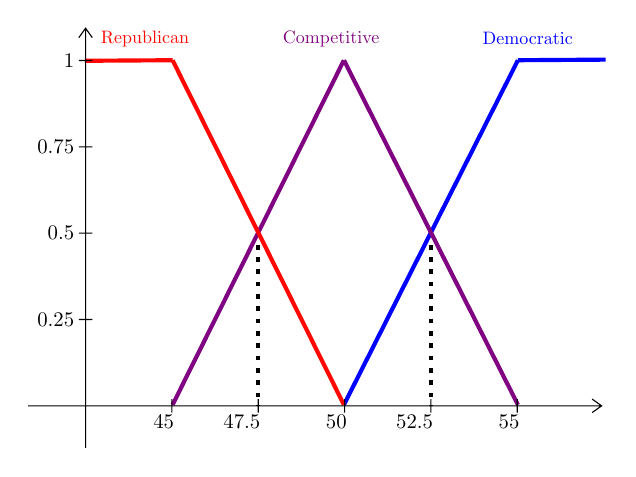
\begin{tikzpicture}[x=0.75pt,y=0.75pt,yscale=-0.65,xscale=0.65]
		%uncomment if require: \path (0,343); %set diagram left start at 0, and has height of 343
		
		%Straight Lines [id:da1804173767960917] 
		\draw [line width=1.5]  [dash pattern={on 1.69pt off 2.76pt}]  (240.93,180.71) -- (240.93,309) ;
		%Straight Lines [id:da44128725993068696] 
		\draw [color={rgb, 255:red, 0; green, 0; blue, 255 }  ,draw opacity=1 ][line width=1.5]    (433.43,53) -- (498.43,52.57) ;
		%Straight Lines [id:da616789366030722] 
		\draw [line width=1.5]  [dash pattern={on 1.69pt off 2.76pt}]  (368.93,180.71) -- (368.93,309) ;
		%Straight Lines [id:da9824154573362276] 
		\draw [color={rgb, 255:red, 0; green, 0; blue, 255 }  ,draw opacity=1 ][line width=1.5]    (433.43,53) -- (304.43,308.43) ;
		%Straight Lines [id:da32445679508513114] 
		\draw [color={rgb, 255:red, 128; green, 4; blue, 129 }  ,draw opacity=1 ][line width=1.5]    (304.43,53) -- (433.43,308.43) ;
		%Straight Lines [id:da8940161641483833] 
		\draw [color={rgb, 255:red, 128; green, 4; blue, 129 }  ,draw opacity=1 ][line width=1.5]    (304.43,53) -- (177.43,308.43) ;
		%Straight Lines [id:da8163094628355578] 
		\draw [color={rgb, 255:red, 255; green, 8; blue, 3 }  ,draw opacity=1 ][line width=1.5]    (177.43,53) -- (304.43,308.43) ;
		%Straight Lines [id:da09373912387885808] 
		\draw [color={rgb, 255:red, 255; green, 8; blue, 3 }  ,draw opacity=1 ][line width=1.5]    (112.43,53.43) -- (177.43,53) ;
		%Shape: Axis 2D [id:dp7314167760669636] 
		\draw  (70.43,309.19) -- (495.43,309.19)(112.93,29.29) -- (112.93,340.29) (488.43,304.19) -- (495.43,309.19) -- (488.43,314.19) (107.93,36.29) -- (112.93,29.29) -- (117.93,36.29) (176.93,304.19) -- (176.93,314.19)(240.93,304.19) -- (240.93,314.19)(304.93,304.19) -- (304.93,314.19)(368.93,304.19) -- (368.93,314.19)(432.93,304.19) -- (432.93,314.19)(107.93,245.19) -- (117.93,245.19)(107.93,181.19) -- (117.93,181.19)(107.93,117.19) -- (117.93,117.19)(107.93,53.19) -- (117.93,53.19) ;
		\draw   (183.93,321.19) node[anchor=east, scale=0.75]{45} (247.93,321.19) node[anchor=east, scale=0.75]{47.5} (311.93,321.19) node[anchor=east, scale=0.75]{50} (375.93,321.19) node[anchor=east, scale=0.75]{52.5} (439.93,321.19) node[anchor=east, scale=0.75]{55} (109.93,245.19) node[anchor=east, scale=0.75]{0.25} (109.93,181.19) node[anchor=east, scale=0.75]{0.5} (109.93,117.19) node[anchor=east, scale=0.75]{0.75} (109.93,53.19) node[anchor=east, scale=0.75]{1} ;
		
		% Text Node
		\draw (406,31) node [anchor=north west][inner sep=0.75pt]  [color={rgb, 255:red, 0; green, 0; blue, 255 }  ,opacity=1, xscale=0.65,yscale=0.65] [align=left] {Democratic};
		% Text Node
		\draw (258,30) node [anchor=north west][inner sep=0.75pt]  [color={rgb, 255:red, 128; green, 4; blue, 129 }  ,opacity=1,xscale=0.65,yscale=0.65 ] [align=left] {Competitive};
		% Text Node
		\draw (123,30) node [anchor=north west][inner sep=0.75pt]  [color={rgb, 255:red, 255; green, 8; blue, 3 }  ,opacity=1,xscale=0.65,yscale=0.65 ] [align=left] {Republican};
	\end{tikzpicture}
	\caption{Schema of the fuzzy partition designed for the linguistic variable \textit{Voters}.}\label{fig:VotersLinguisticVariable}
\end{figure}

% Analysis of subgroups
Let us start analyzing the results obtained by the subgroup discovery algorithms SDFIOE and GSDFIW. According to the discussion in Section \ref{subsection:SD:general_study} we have considered the following parameters: $MaxFeatures=5$, $\alpha=0.1$, $I=\IGG$, $T=\TP$ and $\lambda=0.85$. The results are collected in Tables \ref{table:usa:SDFIOE} and \ref{table:usa:GSDFIW}, respectively. 

\begin{table}[htp!]
	\centering
	\setlength\tabcolsep{7pt}
	\renewcommand{\arraystretch}{1.75} \large
	\subfloat[Voters $=$ {\color{RRed}Republican}.]{
		\resizebox{\textwidth}{!}{
	\begin{tabular}{l|r|c|c|c|c|}
		\cline{2-6}
		& \multicolumn{1}{c|}{\textbf{IF-THEN Rule}}                                & \textbf{FCoverage} & \textbf{FSupport} & \textbf{FConfidence} & \textbf{FWRAcc} \\ \cline{2-6} 
		& IF ( Evangelicals IS H ) THEN Voters IS Republican                          & 0.315              & 0.213             & 0.676                & 0.070           \\ \cline{2-6} 
		& IF ( University\_Grad IS L ) THEN Voters IS Republican                           & 0.196              & 0.156             & 0.795                & 0.067           \\ \cline{2-6} 
		& IF ( HighSchool\_Grad IS L ) THEN Voters IS Republican                      & 0.253              & 0.178             & 0.707                & 0.063           \\ \cline{2-6} 
		& IF ( Salary IS L ) THEN Voters IS Republican                              & 0.301              & 0.196             & 0.651                & 0.059           \\ \cline{2-6} 
		& IF ( Evangelicals IS H AND Mormons IS L ) THEN Voters IS Republican        & 0.147              & 0.118             & 0.803                & 0.051           \\ \cline{2-6} 
		& IF ( Evangelicals IS H AND HighSchool\_Grad IS L ) THEN Voters IS Republican & 0.112              & 0.102             & 0.911                & 0.051           \\ \cline{2-6} 
		& IF ( HighSchool\_Grad IS L AND Women IS H ) THEN Voters IS Republican     & 0.147              & 0.118             & 0.800                & 0.051           \\ \cline{2-6} 
		& IF ( Blacks IS M AND HighSchool\_Grad IS L ) THEN Voters IS Republican        & 0.105              & 0.094             & 0.893                & 0.046           \\ \cline{2-6} 
		& IF ( Asians IS L ) THEN Voters IS Republican                                 & 0.464              & 0.254             & 0.546                & 0.042           \\ \cline{2-6} 
		& IF ( Evangelicals IS H AND Salary IS L ) THEN Voters IS Republican         & 0.111              & 0.092             & 0.835                & 0.042           \\ \cline{2-6} 
	\end{tabular}
		}
	}
	\\
	\vspace{0.5cm}
	\subfloat[Voters $=$ {\color{CPurple} Competitive}.]{
		\resizebox{\textwidth}{!}{
\begin{tabular}{l|r|c|c|c|c|}
	\cline{2-6}
	& \multicolumn{1}{c|}{\textbf{IF-THEN Rule}}                          & \textbf{FCoverage} & \textbf{FSupport} & \textbf{FConfidence} & \textbf{FWRAcc} \\ \cline{2-6} 
	& IF ( Density IS L ) THEN Voters IS Competitive                      & 0.264              & 0.093             & 0.354                & 0.052           \\ \cline{2-6} 
	& IF ( Asians IS L ) THEN Voters IS Competitive                          & 0.464              & 0.121             & 0.260                & 0.048           \\ \cline{2-6} 
	& IF ( Asians IS L AND Density IS L ) THEN Voters IS Competitive        & 0.134              & 0.066             & 0.492                & 0.045           \\ \cline{2-6} 
	& IF ( Asians IS L AND Evangelicals IS M ) THEN Voters IS Competitive     & 0.136              & 0.064             & 0.474                & 0.043           \\ \cline{2-6} 
	& IF ( Asians IS L AND University\_Grad IS M ) THEN Voters IS Competitive      & 0.185              & 0.071             & 0.386                & 0.042           \\ \cline{2-6} 
	& IF ( Evangelicals IS M ) THEN Voters IS Competitive                   & 0.276              & 0.085             & 0.308                & 0.041           \\ \cline{2-6} 
	& IF ( Asians IS L AND Catholics IS H ) THEN Voters IS Competitive       & 0.150              & 0.065             & 0.432                & 0.041           \\ \cline{2-6} 
	& IF ( Asians IS L AND HighSchool\_Grad IS H ) THEN Voters IS Competitive & 0.213              & 0.074             & 0.349                & 0.041           \\ \cline{2-6} 
	& IF ( Asians IS L AND Veterans IS M ) THEN Voters IS Competitive       & 0.134              & 0.061             & 0.454                & 0.040           \\ \cline{2-6} 
	& IF ( Catholics IS H ) THEN Voters IS Competitive                     & 0.321              & 0.089             & 0.276                & 0.038           \\ \cline{2-6} 
\end{tabular}
		}
	}

	\vspace{0.5cm}
\subfloat[Voters $=$ {\color{DBlue}Democratic}.]{
	\resizebox{\textwidth}{!}{
\begin{tabular}{l|r|c|c|c|c|}
	\cline{2-6}
	& \multicolumn{1}{c|}{\textbf{IF-THEN Rule}}                        & \textbf{FCoverage} & \textbf{FSupport} & \textbf{FConfidence} & \textbf{FWRAcc} \\ \cline{2-6} 
	& IF ( University\_Grad IS H ) THEN Voters IS Democratic                   & 0.350              & 0.237             & 0.678                & 0.102           \\ \cline{2-6} 
	& IF ( Evangelicals IS L ) THEN Voters IS Democratic                  & 0.202              & 0.175             & 0.866                & 0.097           \\ \cline{2-6} 
	& IF ( University\_Grad IS H AND Women IS H ) THEN Voters IS Democratic  & 0.161              & 0.143             & 0.885                & 0.080           \\ \cline{2-6} 
	& IF ( Salary IS H ) THEN Voters IS Democratic                      & 0.314              & 0.201             & 0.641                & 0.080           \\ \cline{2-6} 
	& IF ( Catholics IS H ) THEN Voters IS Democratic                    & 0.321              & 0.197             & 0.614                & 0.073           \\ \cline{2-6} 
	& IF ( Density IS H ) THEN Voters IS Democratic                     & 0.119              & 0.119             & 1.000                & 0.073           \\ \cline{2-6} 
	& IF ( Asians IS M ) THEN Voters IS Democratic                         & 0.244              & 0.166             & 0.681                & 0.072           \\ \cline{2-6} 
	& IF ( Evangelicals IS L AND Women IS H ) THEN Voters IS Democratic & 0.135              & 0.124             & 0.917                & 0.072           \\ \cline{2-6} 
	& IF ( Density IS H AND Women IS H ) THEN Voters IS Democratic    & 0.113              & 0.113             & 1.000                & 0.069           \\ \cline{2-6} 
	& IF ( Hispanics IS M and University\_Grad IS H ) THEN Voters IS Democratic & 0.176              & 0.136             & 0.775                & 0.068           \\ \cline{2-6} 
\end{tabular}
	}
}
	\caption{Subgroups discovered by the algorithm SDFIOE with $MaxFeatures=5$, $k=10$, $\alpha=0.1$, a FCM partition for the features, $I=\IGG$ and $T=\TP$ for the dataset USA2012.}\label{table:usa:SDFIOE}
\end{table}

\begin{table}[htp!]
	\centering
	\setlength\tabcolsep{7pt}
	\renewcommand{\arraystretch}{1.75} \large
	\subfloat[Voters $=$ {\color{RRed}Republican}.]{
		\resizebox{\textwidth}{!}{
	\begin{tabular}{l|r|c|c|c|c|}
		\cline{2-6}
		& \multicolumn{1}{c|}{\textbf{IF-THEN Rule}}                            & \textbf{FCoverage} & \textbf{FSupport} & \textbf{FConfidence} & \textbf{FWRAcc} \\ \cline{2-6} 
		& IF ( Evangelicals IS H ) THEN Voters IS Republican                      & 0.315              & 0.213             & 0.676                & 0.070           \\ \cline{2-6} 
		& IF ( University\_Grad IS L ) THEN Voters IS Republican                       & 0.196              & 0.156             & 0.795                & 0.067           \\ \cline{2-6} 
		& IF ( HighSchool\_Grad IS L ) THEN Voters IS Republican                  & 0.253              & 0.178             & 0.707                & 0.063           \\ \cline{2-6} 
		& IF ( Salary IS L ) THEN Voters IS Republican                          & 0.301              & 0.196             & 0.651                & 0.059           \\ \cline{2-6} 
		& IF ( Evangelicals IS H AND Mormons IS L ) THEN Voters IS Republican    & 0.147              & 0.118             & 0.803                & 0.051           \\ \cline{2-6} 
		& IF ( HighSchool\_Grad IS L AND Women IS H ) THEN Voters IS Republican & 0.147              & 0.118             & 0.800                & 0.051           \\ \cline{2-6} 
		& IF ( Asians IS L ) THEN Voters IS Republican                             & 0.464              & 0.254             & 0.546                & 0.042           \\ \cline{2-6} 
		& IF ( Women IS L ) THEN Voters IS Republican                          & 0.211              & 0.136             & 0.642                & 0.039           \\ \cline{2-6} 
		& IF ( Catholics IS L ) THEN Voters IS Republican                        & 0.160              & 0.107             & 0.670                & 0.034           \\ \cline{2-6} 
		& IF ( Veterans IS H ) THEN Voters IS Republican                        & 0.422              & 0.216             & 0.513                & 0.024           \\ \cline{2-6} 
	\end{tabular}
		}
	}
	\\
	\vspace{0.5cm}
	\subfloat[Voters $=$ {\color{CPurple} Competitive}.]{
		\resizebox{\textwidth}{!}{
			\begin{tabular}{l|r|c|c|c|c|}
				\cline{2-6}
				& \multicolumn{1}{c|}{\textbf{IF-THEN Rule}}                                 & \textbf{FCoverage} & \textbf{FSupport} & \textbf{FConfidence} & \textbf{FWRAcc} \\ \cline{2-6} 
				& IF ( Density IS L ) THEN Voters IS Competitive                             & 0.264              & 0.093             & 0.354                & 0.052           \\ \cline{2-6} 
				& IF ( Asians IS L ) THEN Voters IS Competitive                                 & 0.464              & 0.121             & 0.260                & 0.048           \\ \cline{2-6} 
				& IF ( Asians IS L AND Evangelicals IS M ) THEN Voters IS Competitive            & 0.136              & 0.064             & 0.474                & 0.043           \\ \cline{2-6} 
				& IF ( Asians IS L AND University\_Grad IS M ) THEN Voters IS Competitive             & 0.185              & 0.071             & 0.386                & 0.042           \\ \cline{2-6} 
				& IF ( Evangelicals IS M ) THEN Voters IS Competitive                          & 0.276              & 0.085             & 0.308                & 0.041           \\ \cline{2-6} 
				& IF ( Protestants IS H ) THEN Voters IS Competitive                         & 0.256              & 0.076             & 0.296                & 0.035           \\ \cline{2-6} 
				& IF ( Retired IS L AND Veterans IS H ) THEN Voters IS Competitive         & 0.122              & 0.051             & 0.421                & 0.032           \\ \cline{2-6} 
				& IF ( Evangelicals IS H ) THEN Voters IS Competitive                          & 0.315              & 0.077             & 0.245                & 0.027           \\ \cline{2-6} 
				& IF ( Evangelicals IS M AND HighSchool\_Grad IS H ) THEN Voters IS Competitive & 0.188              & 0.057             & 0.302                & 0.027           \\ \cline{2-6} 
				& IF ( Veterans IS H ) THEN Voters IS Competitive                            & 0.422              & 0.091             & 0.215                & 0.024           \\ \cline{2-6} 
			\end{tabular}
		}
	}
	
	\vspace{0.5cm}
	\subfloat[Voters $=$ {\color{DBlue}Democratic}.]{
		\resizebox{\textwidth}{!}{
		\begin{tabular}{l|r|c|c|c|c|}
			\cline{2-6}
			& \multicolumn{1}{c|}{\textbf{IF-THEN Rule}}                        & \textbf{FCoverage} & \textbf{FSupport} & \textbf{FConfidence} & \textbf{FWRAcc} \\ \cline{2-6} 
			& IF ( University\_Grad IS H ) THEN Voters IS Democratic                   & 0.350              & 0.237             & 0.678                & 0.102           \\ \cline{2-6} 
			& IF ( Evangelicals IS L ) THEN Voters IS Democratic                  & 0.202              & 0.175             & 0.866                & 0.097           \\ \cline{2-6} 
			& IF ( Salary IS H ) THEN Voters IS Democratic                      & 0.314              & 0.201             & 0.641                & 0.080           \\ \cline{2-6} 
			& IF ( Catholics IS H ) THEN Voters IS Democratic                    & 0.321              & 0.197             & 0.614                & 0.073           \\ \cline{2-6} 
			& IF ( Density IS H ) THEN Voters IS Democratic                     & 0.119              & 0.119             & 1.000                & 0.073           \\ \cline{2-6} 
			& IF ( Evangelicals IS L AND Women IS H ) THEN Voters IS Democratic & 0.135              & 0.124             & 0.917                & 0.072           \\ \cline{2-6} 
			& IF ( HighSchool\_Grad IS H ) THEN Voters IS Democratic              & 0.460              & 0.236             & 0.512                & 0.058           \\ \cline{2-6} 
			& IF ( Salary IS M ) THEN Voters IS Democratic                      & 0.204              & 0.106             & 0.521                & 0.027           \\ \cline{2-6} 
			& IF ( Mormons IS M AND Veterans IS H ) THEN Voters IS Democratic  & 0.151              & 0.077             & 0.510                & 0.019           \\ \cline{2-6} 
			& IF ( Catholics IS M ) THEN Voters IS Democratic                    & 0.297              & 0.126             & 0.424                & 0.011           \\ \cline{2-6} 
		\end{tabular}
		}
	}
	\caption{Subgroups discovered by the algorithm GSDFIW with $MaxFeatures=5$, $k=10$ $\alpha=0.1$, a FCM partition for the features, $I=\IGG$, $T=\TP$ and $\lambda=0.85$ for the dataset USA2012.}\label{table:usa:GSDFIW}
\end{table}

With respect to the subgroups obtained for the Republican label, i.e., subgroups where the target are solid Republican states (Panels (a) in Tables \ref{table:usa:SDFIOE} and \ref{table:usa:GSDFIW}), several remarks can be 
highlighted. Indeed, many of the subgroups involve the following pairs (feature,linguistic label):
\begin{itemize}
	\item (Evangelicals,High): If a state has a high percentage of people who identify themselves as evangelical, then the state is solid Republican. This subgroup is a direct consequence of the historical alignment of this group with the Republican Party (see \cite{pewresearch,Schwadel2017}).
	\item (University\_Grad,Low) or (HighSchool\_Grad,Low): If a state has a low percentage of graduates either in High School or University, then the state is solid Republican. Indeed, several researchers have also noticed that the education level of a voter is a key factor on the U.S. elections and the Republican Party performs much better among non-high school educated voters \cite{Harris2018}.
	\item (Salary,Low): If the state has a low median average annual household income, then the state is solid Republican. This subgroup highlights the division on American politics where Republicans shine on rural (not-so-developed) states where the annual income is not as high as it is in many urban states (mostly Democratic) \cite{Molinaro2021}.
\end{itemize}
Note that there are some differences between the results obtained by both algorithms. While many subgroups of SDFIOE involve (HighSchool\_Grad,Low) or (Evangelicals,High) with a significant overlap among subgroups, this overlap is attenuated drastically by GSDFIW, leading to new subgroups which involve other pairs such as (Veterans,High) and (Women,Low). These subgroups make also a lot of sense since ex-members of the Armed forces vote overwhelmingly the Republican Party while women tend to vote more for the Democrat Party.

 With respect to the subgroups obtained for the Democratic label, i.e., subgroups where the target are solid Democratic states, the following pairs (feature,linguistic label) play a main role:
\begin{itemize}
	\item (University\_Grad,High), (Evangelicals,Low), (Women,High) and (Salary,High): These pairs have opposite labels than the ones already described for the Republican class, leading to an opposite effect on the vote. Namely, university graduates, women and states with a high median average annual household income or a low percentage of evangelicals tend to prefer the Democratic Party.
	\item (Density,High): If the density of a state is high, then the state is solid Democratic. The Democratic Party obtains great results in both coasts where states with the important U.S. cities are located: Eastern coast with Washington, New York, Philadelphia, etc.; Western coast with Los Angeles, San Diego, San Francisco, Seattle, etc. These states are very populated with a higher density than other more rural states.
	\item (Catholics,High): If the percentage of people who identify themselves with the Catholic church is high, the state is solid Democratic. The political alignment of Catholics is not so biased as the one of Evangelicals, becoming one of the main swing groups in elections. In \cite{pewresearchB} a study concluded that the Democratic Party obtained 52\% of votes among Catholics in 2012. However, in 2016 they favored the Republican Party, while in 2020 the Democratic Party gained the upper hand \cite{Newport2020}.
	\item (Asians,Medium) or (Hispanics,Medium): Historically, immigrants tend to vote for the Democratic Party. However, while Asians are a cohesive group, there are different subgroups among Hispanics depending on their country of origin. Cuban immigrants tend to vote for the Republican Party since they fled from the Cuban regime, while other Hispanics prefer the Democratic Party \cite{pewresearchC}.
\end{itemize}

%Moreover, there exist only 9 swing states.
The third analysis corresponds to the subgroups of the Competitive label, i.e., subgroups where the target are swing states. It should be noted that the $FWRAcc$ values of the subgroups found for this label are smaller in general than the ones obtained for the other linguistic labels. Therefore, the quality of the subgroups is smaller and their possible interpretation is more complex. In these subgroups, the following pairs (feature,linguistic label) are mostly considered:
\begin{itemize}
	\item (Density,Low) or (Asians, Low): These subgroups state that if either the Density of a state or its percentage of Asians is low, then the state is competitive. These subgroups must be analyzed cautiously due to the presence of extreme outliers in the Density and the Asians variables (see Figure \ref{fig:boxplots}). Take for instance the Asians variable. Hawaii has a 38.6\% of Asians, a much higher value than any other state in which many of them have percentages under 10\%. Therefore, most of the states with a high membership value of the class ``Competitive'' have also a high membership value to the label Low of the Asians variable. In fact, this is also true in general for those states with high membership values to the other classes. Therefore, the pair (Asians,Low) is over-represented and the subgroups involving this pair have relatively significant $FWRAcc$ values but their importance can be neglected. A similar analysis can be done for (Density,Low).  
	\item (Evangelicals,Medium) or (University\_Grad,Medium): These pairs indicate that when the presence of very strong aligned groups (Evangelicals for Republicans; University\_Grad for Democrats) is average, then the state is competitive. Notice that the pair (Evangelicals,High) is also considered, but the corresponding subgroup has a lower $FWRAcc$.
	\item (Protestants,High): This subgroup points out that if the percentage of non-evangelical Protestants is significantly high then the state is competitive. This rule stands out with respect to others for two reasons: the variable Protestants does not appear in any of the subgroups obtained for the Democratic or Republican labels, and this subgroup is disclosed only when the weighted covering algorithm is applied. The knowledge captured by this rule is supported by \cite{Schwadel2017}, in which it is concluded that while Evangelicals have increased their alignment with the Republican Party over the past elections, there has been a decline in Republican affiliation and voting among non-evangelical Protestants.
\end{itemize}

\begin{figure}[ht]
	\centering
	\begin{subfigure}{.4\textwidth}
		\centering
		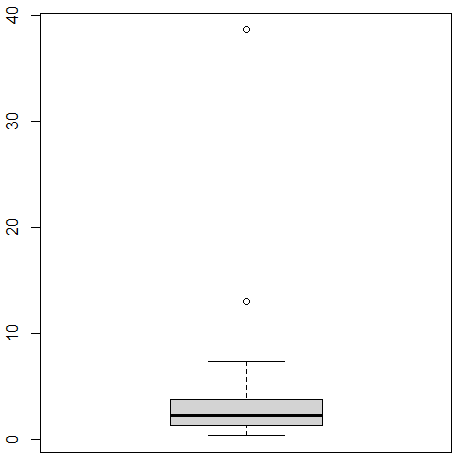
\includegraphics[scale=0.4]{boxplot_asia.png}
		\caption{Asians.}
	\end{subfigure}\hspace{0.5cm}
	\begin{subfigure}{.4\textwidth}
		\centering
		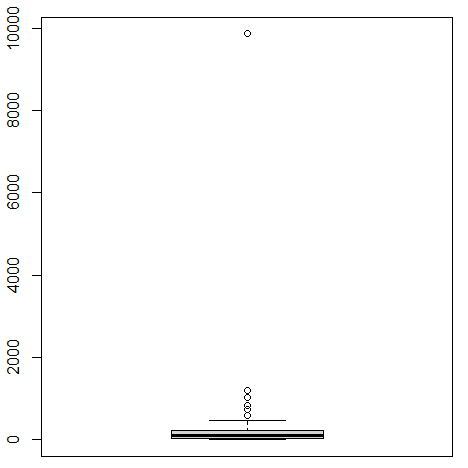
\includegraphics[scale=0.4]{boxplot_density.png}
		\caption{Density.}
	\end{subfigure}
	\caption{Box plot of the variables ``Asians'' and ``Density'' of the database USA2012.}
	\label{fig:boxplots}
\end{figure}

% Comparison
At this point, we focus on the comparison of our SD algorithms with other existing approaches. As we commented in Section \ref{section:SD:introduction}, there exist several SD algorithms based on fuzzy rules and even an RStudio package is available \cite{SDEFSR}. Nonetheless, according to the corresponding implementations any comparison presents some inconveniences:
\begin{itemize}
	\item In these algorithms the target is considered to be a categorical variable, not a fuzzy linguistic variable.
	\item The fuzzy uniform partitioning method is determined by default and the documentation does not clearly specify how a custom fuzzy partition for the numeric variables can be provided.
	\item The implementation does not provide flexibility in the selection of the fuzzy operators and mainly the minimum t-norm is determined by default.
	\item Generally, in these algorithms the authors have focused in optimizing the measure confidence with a minimum support pruning, for which they provide a fuzzy interpretation. Although the option for optimizing $WRAcc$ is available, this measure does not have the same interpretation as the one provided in this chapter (see the discussion in Section \ref{subsection:quality_measures}).
	\item The algorithms focus on dealing with big datasets using sophisticated search heuristics based on evolutionary algorithms.
\end{itemize}
To exemplify this scenario, we have executed the algorithms SDIGA \cite{delJesus2007}, MESDIF \cite{Berlanga2006,delJesus2007B,Carmona2011} and NMEEF-SD \cite{Carmona2010} selecting the optimization of the quality measure $WRAcc$ and the by-default parameters. Since these algorithms are only valid for categorical targets, the variable ``Voters'' has been discretized by assigning to each state the label of the fuzzy set for which it has a maximum membership degree according to the fuzzy partition designed (see Figure \ref{fig:VotersLinguisticVariable}). The rest of the variables have been fuzzified according to the corresponding implementation, i.e., with a uniform partition. In order to make a fair comparison, we have rerun our algorithms SDFIOE and GSDFIW with $MaxFeatures=5$, $k=5$, $\alpha=0.1$, $I=\IGD$, $T=\TM$, $\lambda=0.85$, and also the uniform fuzzy partitioning method for the feature variables. In Tables \ref{table:usa:comparison:Fuzzy} and \ref{table:usa:comparison:Fuzzy2} the subgroups obtained for the target class ``Republican'' in all five cases can be found. We have omitted the results for the two other labels since the conclusions of the comparison were similar. It is very noticeable that in all cases the obtained subgroups are dominated by the pairs (Density,Low) and (Asians,Low) and the results are very different from the ones in Tables \ref{table:usa:SDFIOE} and \ref{table:usa:GSDFIW}. From the box plot of these two variables we can observe that they have marked outliers (see Figure \ref{fig:boxplots}). This situation clearly affects the performance of all five algorithms because a uniform fuzzy partition was used. Indeed, the obtained rules are fruitless in comparison with the discussion of the results in Tables \ref{table:usa:SDFIOE} and \ref{table:usa:GSDFIW} in which the FCM partitioning method was considered. This clearly emphasizes again the importance of the selection of the fuzzy operators and the fuzzy partitions. Besides, the algorithms SDIGA, MESDIF and NMEEF-SD only provide the fuzzy generalization of the measures support and confidence, but the coverage and $WRAcc$ have a crisp meaning. In any case, none of the measures are comparable with ours since the definitions of fuzzy support and confidence introduced in this chapter depend on the choice of the fuzzy implication function.

\begin{table}[htp!]
	\centering
	\setlength\tabcolsep{7pt}
	\renewcommand{\arraystretch}{1.75} \large
	\subfloat[SDIGA.]{
		\resizebox{\textwidth}{!}{
	\begin{tabular}{|r|c|c|c|c|}
		\hline
		\multicolumn{1}{|c|}{\textbf{IF-THEN Rule}}                   & \textbf{Coverage} & \textbf{FSupport} & \textbf{FConfidence} & \textbf{WRAcc} \\ \hline
		IF ( Density IS L ) THEN Voters IS Republican & 0.980  & 0.445 & 0.472 &  0.009 \\ \hline
	\end{tabular}
}
	}
	
	\vspace{0.5cm}
	\subfloat[MESDIF.]{
		\resizebox{\textwidth}{!}{
			\begin{tabular}{|r|c|c|c|c|}
				\hline
				\multicolumn{1}{|c|}{\textbf{IF-THEN Rule}}                   & \textbf{Coverage} & \textbf{FSupport} & \textbf{FConfidence} & \textbf{WRAcc} \\ \hline
				IF ( Asians IS L AND Density IS L ) THEN Voters IS Republican      & 0.941  & 0.417 & 0.503 &  0.027 \\ \hline
				IF ( Asians IS L ) THEN Voters IS Republican                    & 0.961  & 0.417 & 0.490 &  0.018 \\ \hline
				IF ( Density IS L ) THEN Voters IS Republican & 0.980  & 0.445 & 0.472 &  0.009 \\ \hline
			\end{tabular}
		}
	}
\vspace{0.5cm}
	\subfloat[NMEEF-SD.]{
	\resizebox{\textwidth}{!}{
		\begin{tabular}{|r|c|c|c|c|}
			\hline
			\multicolumn{1}{|c|}{\textbf{IF-THEN Rule}}                   & \textbf{Coverage} & \textbf{FSupport} & \textbf{FConfidence} & \textbf{WRAcc} \\ \hline
			IF ( Asians IS L AND Density IS L ) THEN Voters IS Republican      & 0.941  & 0.417 & 0.503 &  0.027 \\ \hline
			IF ( Asians IS L ) THEN Voters IS Republican                    & 0.961  & 0.417 & 0.490 &  0.018 \\ \hline
			IF ( Density IS L ) THEN Voters IS Republican & 0.980  & 0.445 & 0.472 &  0.009 \\ \hline
		\end{tabular}
	}
}
	\caption{Subgroups discovered by the algorithms SDIGA, MESDIF and NMEEF-SD setting the optimization of $WRAcc$ and the target class ``Republican'' for the dataset USA2012.}\label{table:usa:comparison:Fuzzy}
\end{table}

\begin{table}[htp!]
	\centering
	\setlength\tabcolsep{7pt}
	\renewcommand{\arraystretch}{1.75} \large
	\subfloat[SDFIOE.]{
		\resizebox{\textwidth}{!}{
			\begin{tabular}{|r|c|c|c|c|}
				\hline
				\multicolumn{1}{|c|}{\textbf{IF-THEN Rule}}                   & \textbf{FCoverage} & \textbf{FSupport} & \textbf{FConfidence} & \textbf{FWRAcc} \\ \hline
				IF ( Asians IS L AND Density IS L AND Hispanics IS L AND University\_Grad IS L ) THEN Voters IS Republican & 0.344  & 0.248 & 0.722 &  0.092 \\ \hline
				IF ( Asians IS L AND Hispanics IS L AND University\_Grad IS L ) THEN Voters IS Republican & 0.344  & 0.248 & 0.722 &  0.092 \\ \hline
				IF ( Density IS L AND Hispanics IS L AND University\_Grad IS L ) THEN Voters IS Republican & 0.350  & 0.248 & 0.722 &  0.089 \\ \hline
				IF ( Hispanics IS L AND University\_Grad IS L ) THEN Voters IS Republican & 0.350  & 0.248 & 0.722 &  0.089 \\ \hline
				IF ( Asians IS L and Density IS L AND University\_Grad IS L ) THEN Voters IS Republican & 0.404  & 0.271 & 0.672 &  0.087 \\ \hline
			\end{tabular}
		}
	}
	
	\vspace{0.5cm}
	\subfloat[GSDFIW.]{
		\resizebox{\textwidth}{!}{
			\begin{tabular}{|r|c|c|c|c|}
			\hline
			\multicolumn{1}{|c|}{\textbf{IF-THEN Rule}}                   & \textbf{FCoverage} & \textbf{FSupport} & \textbf{FConfidence} & \textbf{FWRAcc} \\ \hline
				IF ( Asians IS L AND Density IS L AND Hispanics IS L AND University\_Grad IS L ) THEN Voters IS Republican & 0.344  & 0.248 & 0.722 &  0.092 \\ \hline
				IF ( Asians IS L AND Hispanics IS L AND University\_Grad IS L ) THEN Voters IS Republican & 0.344  & 0.248 & 0.722 &  0.092 \\ \hline
				IF ( Density IS L AND Hispanics IS L AND University\_Grad IS L ) THEN Voters IS Republican & 0.350  & 0.248 & 0.722 &  0.089 \\ \hline
				IF ( Hispanics IS L AND University\_Grad IS L ) THEN Voters IS Republican & 0.350  & 0.248 & 0.722 &  0.089 \\ \hline
			IF ( Asians IS L AND Retired IS M AND University\_Grad IS L ) THEN Voters IS Republican & 0.361  & 0.243 & 0.674 &  0.079 \\ \hline
		\end{tabular}
		}
	}
	\caption{Subgroups discovered by the algorithms  SDFIOE and GSDFIW with $MaxFeatures=5$, $k=5$, $\alpha=0.1$, $I=\IGD$, $T=\TM$, $\lambda=0.85$ for the dataset USA2012 and the target class ``Republican'' using the uniform partitioning method for the feature variables.}\label{table:usa:comparison:Fuzzy2}
\end{table}


In view of the situation exposed above, we think that as a first approach it is more appropriate to compare our algorithms with classical subgroup discovery algorithms like Apriori-SD \cite{Kavsek2003}, CN2-SD \cite{Lavrac2004} or SD-MAP \cite{Atzmueller2006}. Although these algorithms are designed for categorical variables (both target and features), they focus on the optimization of the weighted relative accuracy with a minimum coverage pruning and its algorithmic design resembles more to our perspective. Indeed, the motivation behind this chapter has been generalizing these well-known algorithms to the fuzzy logic framework in which fuzzy implication functions are used to model the corresponding subgroups.

For SD-MAP we have used the implementation in the \textit{rsubgroup} package for Rstudio \cite{rsubgroup}; for CN2-SD we have used the implementation in the \textit{Orange} toolbox for Python \cite{orange};   and for Apriori-SD we have used the \textit{pysubgroup} package for Python \cite{pysubgroup}. In the three algorithms we have considered a minimum coverage of $0.1$ and a maximum number of features of the antecedent of $5$. Since SD-MAP and Apriori-SD have a Top-$k$ approach we have also selected $k=10$. On the other hand, for the multiplicative weights of CN2-SD we have selected $\gamma=0.85$. Since these algorithms are adequate for categorical variables, in order for the comparison to be more adequate we have discretized all the variables of the database USA2012 by assigning to each state the linguistic label of the fuzzy set for which it has a maximum membership degree according to the fuzzy partition considered for the experiments of Tables \ref{table:usa:SDFIOE} and \ref{table:usa:GSDFIW}. The results for the Republican label are displayed in Table \ref{table:usa:comparison}.

It is important to take into account that an objective and fair comparison between these algorithms and our approach is not possible. Although the goal is similar, the inputs, the description language, the quality measures and the output are different. Thus, the results are not necessarily comparable. Nevertheless, we can provide some conclusions regarding the information that can be extracted from both perspectives.

The subgroups obtained with Apriori-SD and SD-MAP are very similar. In fact, the Top 5 subgroups are exactly the same. This is because both are exhaustive algorithms with the same descriptive language, although in Apriori-SD a post-processing weighting covering schema is implemented. Nonetheless, it is very noticeable that the pairs (Evangelicals,High), (Density,Low), (Mormons,Low) and (Asians,Low) have a leading role. For instance, in both cases the 80\% of subgroups have the pair (Evangelicals,High) in the antecedent. This is due to the high percentage of states that have been classified as evangelical and republican in the discretization of the dataset. In this case, the constraint of needing to discretize the numeric variables has overemphasized some features and this has resulted in subgroups with a lot of overlap and that do not provide as much information as those obtained by our algorithms. Indeed, although in our results in Tables \ref{table:usa:SDFIOE} and \ref{table:usa:GSDFIW} these features also have an important role, our subgroups are much more diverse, they have less overlap and they point out more key features.

On the other hand, the subgroups computed with CN2-SD have the property that negations are allowed in the antecedent. This more general description language enables the existence of subgroups with a higher WRAcc than Apriori-SD and SD-MAP and it also provides more diverse subgroups. Nonetheless, the strong presence of the negation in all the obtained subgroups makes them more complex to analyze. Some of the subgroups obtained by CN2-SD go in the same direction as the ones in our results in Tables \ref{table:usa:SDFIOE} and \ref{table:usa:GSDFIW}, although in both cases the output is clearly different and the overall involved features are not the same. For instance, in our study the pair (Salary,Low) has been interesting to discuss but this pair does not appear in any of the subgroups obtained with CN2-SD. On the other hand, the pair (Unemployment,NOT High) appears in the fourth and tenth position in the list of Top 10 best subgroups obtained by CN2-SD, but the Unemployment variable is not even considered in the results obtained by our algorithms.

At this point, let us highlight the major advantage of our perspective with respect to the rest. Although in the existing algorithms the subgroups are represented as IF-THEN rules, none of these perspectives model subgroups as truly logical conditionals. In our opinion, this negatively affects the interpretability of the subgroups and can generate misconceptions. By incorporating the use of fuzzy implication functions we have not only shown that we disclose valuable knowledge that is not equivalent to that obtained by the existing perspectives, but we have also built a new framework in which the conditional in the description of subgroup inherits the meaning of the conditional within the fuzzy logic. Thus, our modeling allows a more natural interpretation of subgroups according to their description.


\begin{table}[htp!]
	\centering
	\setlength\tabcolsep{7pt}
	\renewcommand{\arraystretch}{1.75} \large
	\subfloat[APRIORI-SD.]{
		\resizebox{\textwidth}{!}{
		\begin{tabular}{|r|c|c|c|c|}
			\hline
			\multicolumn{1}{|c|}{\textbf{IF-THEN Rule}}           & \textbf{Coverage} & \textbf{Support} & \textbf{Confidence} & \textbf{WRAcc} \\ \hline
			IF ( Evangelicals IS H AND Mormons IS L ) THEN Voters IS Republican                         & 0.294  & 0.255 & 0.867 &  0.122 \\ \hline
			IF ( Density IS L AND Evangelicals IS H AND Mormons IS L ) THEN Voters IS Republican             & 0.294  & 0.255 & 0.867 &  0.122 \\ \hline
			IF ( Asians IS L AND University\_Grad IS L ) THEN Voters IS Republican       & 0.255  & 0.235 & 0.923 &  0.120 \\ \hline
			IF ( Asians IS L AND Density IS L AND University\_Grad IS L ) THEN Voters IS Republican       & 0.255  & 0.235 & 0.923 &  0.120 \\ \hline
			IF ( Density IS L AND Evangelicals IS H AND Hispanics IS L AND Mormons IS L ) THEN Voters IS Republican & 0.216  & 0.216 & 1.000 &  0.118 \\ \hline
			IF ( Asians IS L AND Density IS L AND Evangelicals IS H AND Hispanics IS L ) THEN Voters IS Republican& 0.216  & 0.216 & 1.000 &  0.118 \\ \hline
			IF ( Asians IS L AND Evangelicals IS H AND Hispanics IS L ) THEN Voters IS Republican  & 0.216  & 0.216 & 1.000 &  0.118 \\ \hline
			IF ( Density IS L AND Evangelicals IS H AND Hispanics IS L ) THEN Voters IS Republican   & 0.216  & 0.216 & 1.000 &  0.118 \\ \hline
			IF ( Evangelicals IS H AND Hispanics IS L ) THEN Voters IS Republican   & 0.216  & 0.216 & 1.000 &  0.118 \\ \hline
			IF ( Evangelicals IS H AND Hispanics IS L AND Mormons IS L ) THEN Voters IS Republican   & 0.216  & 0.216 & 1.000 &  0.118 \\ \hline
		\end{tabular}
	}
}
	
	\vspace{0.5cm}
	\subfloat[SD-MAP.]{
		\resizebox{\textwidth}{!}{
\begin{tabular}{|r|c|c|c|c|}
	\hline
	\multicolumn{1}{|c|}{\textbf{IF-THEN Rule}}                   & \textbf{Coverage} & \textbf{Support} & \textbf{Confidence} & \textbf{WRAcc} \\ \hline
	IF ( Evangelicals IS H AND Mormons IS L ) THEN Voters IS Republican & 0.294  & 0.255 & 0.867 &  0.122 \\ \hline
	IF ( Density IS L AND Evangelicals IS H AND Mormons IS L ) THEN Voters IS Republican                    & 0.294  & 0.255 & 0.867 &  0.122 \\ \hline
	IF ( Asians IS L AND University\_Grad IS L ) THEN Voters IS Republican      & 0.255  & 0.235 & 0.923 &  0.120 \\ \hline
	IF ( Asians IS L AND Density IS L AND University\_Grad IS L ) THEN Voters IS Republican   & 0.255  & 0.235 & 0.923 &  0.120 \\ \hline
	IF ( Density IS L IS Evangelicals IS H AND Hispanics IS L AND Mormons IS L ) THEN Voters IS Republican & 0.216  & 0.216 & 1.000 &  0.118 \\ \hline
	\begin{tabular}[c]{@{}r@{}} IF ( Asians IS L AND Density IS L AND Evangelicals IS H \\ AND Hispanics IS L AND Mormons IS L ) THEN Voters IS Republican \end{tabular} & 0.216  & 0.216 & 1.000 &  0.118 \\ \hline
	IF ( Asians IS L AND Density IS L AND Evangelicals IS H AND Hispanics IS L ) THEN Voters IS Republican  & 0.216  & 0.216 & 1.000 &  0.118 \\ \hline
	IF ( Evangelicals IS H AND Hispanics IS L AND Mormons IS L ) THEN Voters IS Republican   & 0.216  & 0.216 & 1.000 &  0.118 \\ \hline
	IF ( Asians IS L AND Evangelicals IS H AND Hispanics IS L AND Mormons IS L ) THEN Voters IS Republican & 0.216  & 0.216 & 1.000 &  0.118 \\ \hline
	IF ( Asians IS L AND Evangelicals IS H AND Hispanics IS L ) THEN Voters IS Republican & 0.216  & 0.216 & 1.000 &  0.118 \\ \hline
\end{tabular}
		}
	}
\\
\vspace{0.5cm}
	\subfloat[CN2-SD $\gamma=0.85$.]{
	\resizebox{\textwidth}{!}{
		\begin{tabular}{|r|c|c|c|c|}
			\hline
			\multicolumn{1}{|c|}{\textbf{IF-THEN Rule}}                  & \textbf{Coverage}     & \textbf{Support}      & \textbf{Confidence}   & \textbf{WRAcc}        \\ \hline
			IF ( Catholics IS NOT H AND University\_Grad IS NOT H ) THEN Voters IS Republican  & 0.451  & 0.373 & 0.826 &  0.169 \\ \hline
			IF ( Asians IS NOT H AND Catholics IS NOT H AND Density IS L ) THEN Voters IS Republican  & 0.549  & 0.412 & 0.750 &  0.164 \\ \hline 
			IF ( Density IS NOT M  AND  Evangelicals IS NOT L  AND  University\_Grad IS NOT H ) THEN Voters IS Republican   & 0.510  & 0.392 & 0.769 &  0.162 \\ \hline 
			\begin{tabular}[c]{@{}r@{}} IF ( Asians IS NOT H AND Catholics IS NOT H AND Density IS L  \\ AND Unemployment IS NOT H) THEN Voters IS Republican \end{tabular}   & 0.431  & 0.353 & 0.818 &  0.158 \\ \hline 
			\begin{tabular}[c]{@{}r@{}} IF ( Density IS L AND Evangelicals IS NOT L AND University\_Grad IS NOT H \\ AND Veterans IS NOT M ) THEN Voters IS Republican  \end{tabular} & 0.392  & 0.333 & 0.850 & 0.156  \\ \hline 
			IF ( Asians IS NOT H AND Density IS L AND University\_Grad IS NOT H )  THEN Voters IS Republican &  0.569 & 0.412 & 0.724 &  0.155 \\ \hline 
			IF ( Evangelicals IS NOT L AND University\_Grad IS NOT H ) THEN Voters IS Republican & 0.529  & 0.392 & 0.741 &  0.153 \\ \hline 
			\begin{tabular}[c]{@{}r@{}} IF ( Asians IS NOT H AND Catholics IS NOT H AND Density IS L \\ AND Hispanics IS NOT H ) THEN Voters IS Republican \end{tabular}  & 0.490  & 0.373 & 0.760 &  0.151 \\ \hline 
			IF (Asians IS L AND Catholics IS NOT H ) THEN Voters IS Republican  & 0.451  & 0.353 & 0.783 &  0.150 \\ \hline 
			IF ( Asians IS NOT H AND Catholics IS NOT H AND Unemployment IS NOT H ) THEN Voters IS Republican   & 0.451  & 0.353 & 0.783 &  0.150 \\ \hline 
			IF ( Density IS L AND University\_Grad IS NOT H ) THEN Voters IS Republican  & 0.588  & 0.412 & 0.700&  0.146 \\ \hline 
			IF ( Asians IS H AND Density IS L ) THEN Voters IS Republican  & 0.745  & 0.451 & 0.605 &  0.115 \\ \hline 
		\end{tabular}
	}
}
	\caption{Subgroups discovered by the algorithms  Apriori-SD, SD-MAP and CN2-SD for the dataset USA2012 and the target class ``Republican''.}\label{table:usa:comparison}
\end{table}

To end this case of study, we have applied also the STFI algorithm in order to detect interesting sharp transitions with respect to the target variable when a pair (feature,linguistic label) is added to the antecedent of the rule. The algorithm found 178 transitions, the Top 10 ones according to the sharpness value are displayed in Table \ref{table:usa:STFI}. These transitions are specially interesting since they point out key scenarios which are unstable with respect to a certain feature. Indeed, the addition of the corresponding feature to the scenario of the origin fuzzy rule causes a drastic shift to the opposite party. Let us analyze in depth the Top 3 of the transitions:
\begin{itemize}
	\item The first one states that if we add the pair (Catholics,High) to the antecedent of the rule (If (White,High) then (Voters,Republican)) then the consequent is modified to (Voters,Democratic). This transition can be explained due to the vote preferences of these racial and religious groups. We have aforementioned earlier that in the 2012 U.S. Elections Catholics slightly favored the Democratic Party. On the contrary, voters self-identified as white favored the Republican Party \cite{Cillizza2012}. While states with a high percentage of white voters generally went to the Republican column, states with a high percentage of both white and catholic voters (which are North-East and Midwest states) are traditionally Democratic.
	\item  The second one states that if we add the pair (Asians,Low) to the antecedent of the rule (If (Hispanics,Medium) then (Voters,Democratic)) then the consequent is modified to (Voters,Republican). While in general in states with a significant presence of Hispanics the Democratic Party enjoys an advantage, adding the condition that the percentage of Asians is low shifts the focus towards South-East states where Republicans have a stronghold. 
	\item The third transition indicates that if we add the pair (Women,Low) to the antecedent of the rule (If (Salary,High) then (Voters,Democratic)) then the consequent is modified to (Voters,Republican). While states with voters with a higher median average annual household income favor the Democratic Party, adding a low percentage of women in the state moves the focus to some West rural states such as Utah or Wyoming which are exceptions on the rule that in rural states the annual income is lower. These states are solid Republican. 
\end{itemize}  

\begin{table}[htp!]
		\centering
	\setlength\tabcolsep{7pt}
	\renewcommand{\arraystretch}{1.75} \large
		\resizebox{\textwidth}{!}{
\begin{NiceTabular}{|r|r|l|c|c|}[hvlines,colortbl-like]
	\hline
	\multicolumn{1}{|c|}{\textbf{IF-THEN rule origin}}                                                            & \multicolumn{1}{c|}{\textbf{Condition Added}} & \multicolumn{1}{c|}{\textbf{New Consequent}} & \textbf{FCoverage Origin} & \textbf{Sharpness} \\ \hline
	\cellcolor{RRed!30} IF ( White IS H ) THEN Voters IS Republican                                                                  & Catholics IS H                                & \cellcolor{DBlue!30} THEN Voters IS Democratic                     & 0.115                     & 1.167              \\ \hline
	IF ( Hispanics IS M ) THEN Voters IS Democratic \cellcolor{DBlue!30}                                                                & Asians IS L                                     & \cellcolor{RRed!30} THEN Voters IS Republican                     & 0.129                     & 1.157              \\ \hline
	IF ( Salary IS H ) THEN Voters IS Democratic \cellcolor{DBlue!30}                                                                 & Women IS L                                  & \cellcolor{RRed!30} THEN Voters IS Republican                     & 0.110                      & 1.115              \\ \hline
	IF ( Asians IS L ) THEN Voters IS Republican     \cellcolor{RRed!30}                                                                & Salary IS H                                  & THEN Voters IS Democratic \cellcolor{DBlue!30}                    & 0.111                     & 1.093              \\ \hline
	IF ( Asians IS L ) THEN Voters IS Republican \cellcolor{RRed!30}                                                                    & Catholics IS H                                & THEN Voters IS Democratic \cellcolor{DBlue!30}                    & 0.150                      & 1.061              \\ \hline
	IF ( Veterans IS L ) THEN Voters IS Democratic  \cellcolor{DBlue!30}                                                              & Retired IS L                                & THEN Voters IS Republican   \cellcolor{RRed!30}                  & 0.102                     & 1.058              \\ \hline
	IF ( Retired IS M ) THEN Voters IS Republican \cellcolor{RRed!30}                                                               & HighSchool\_Grad IS H                          & THEN Voters IS Democratic  \cellcolor{DBlue!30}                   & 0.110                      & 1.042              \\ \hline
	IF ( Salary IS M ) THEN Voters IS Democratic \cellcolor{DBlue!30}                                                                 & White IS H                                  & THEN Voters IS Republican \cellcolor{RRed!30}                    & 0.103                     & 1.042              \\ \hline
	IF ( Salary IS M ) THEN Voters IS Democratic  \cellcolor{DBlue!30}                                                                & Mormons IS L                                 & THEN Voters IS Republican  \cellcolor{RRed!30}                   & 0.117                     & 1.042              \\ \hline
	\begin{tabular}[c]{@{}r@{}}IF ( HighSchool\_Grad IS H \\ AND Unemployment IS L ) THEN Voters IS Democratic\end{tabular} \cellcolor{DBlue!30} & White IS H                                  & THEN Voters IS Republican  \cellcolor{RRed!30}                   & 0.121                     & 1.041              \\ \hline
\end{NiceTabular}
}

\caption{Top 10 transitions according to $Sharpness$ discovered by the algorithm STFI with $MaxFeatures=5$, $\alpha=0.1$, a FCM partition for the features, $I=\IGG$, $T=\TP$ for the dataset USA2012.}\label{table:usa:STFI}
\end{table}

\section{Conclusions and future work}\label{section:conclusions}

In this chapter, we have presented a novel framework for subgroup discovery based on modeling the logical conditional in the representation of subgroups using fuzzy implication functions. 

First, we have settled the basis of this new perspective. In particular, we have generalized four of the most well-known quality measures in subgroup discovery for fuzzy rules modeled in terms of a t-norm $T$ and a fuzzy implication function $I$. These measures have been denoted by $FCoverage$, $FSupport$, $FConfidence$, and $FWRAcc$. Next, we have thoroughly discussed which additional properties should be satisfied by the pair $(I,T)$ in order to have an adequate behavior when it is used for modeling subgroups. Within this study it has been necessary to introduce a new additional property of fuzzy implication functions related to the generalized modus ponens, which we have denoted by \MTC. Indeed, the property \MTC is needed to interpret $FSupport$ as a measure of generality and it is the key to the optimistic estimate defined for the measure $FWRAcc$. Further, we conclude that a pair $(I,T)$ used for subgroup discovery should satisfy \TC, \MTC and $N_I=\NDOne$. Although a deeper study of the property \MTC has been marked as future work, we have provided several parametric pairs of operators satisfying the three restrictions.

Once we have established the basis for our interpretation of subgroups modeled by fuzzy implication functions, we have focused on the implementation of some subgroup discovery algorithms. In this part, inspired by the classical algorithms, we have implemented exhaustive algorithms based on the optimization of the $FWRAcc$ with a minimum $FCoverage$ pruning. In particular, we have designed three algorithms for searching subgroups: SDFIOE which focuses only on the optimization of $FWRAcc$ using its optimistic estimate; GSDFIW which uses a greedy search but it incorporates a weighted covering algorithm; and WCSDFI which is the weighted covering algorithm designed for GSDFIW but considered as a post-processing technique that can be used in the output of SDFIOE as a faster alternative than using GSDFIW. To complement our subgroup discovery algorithms we have also designed a novel technique based on disclosing pairs of rules with high fuzzy confidence which indicate a change in the target.

In the final part of the chapter, we have tested the applicability of our algorithms from two different points of view. 
First, we have studied its behavior with respect to the input parameters and, specifically, for different fuzzy partitioning methods and pairs $(I,T)$. Regarding the fuzzy partitions, we have reaffirmed what is already well known in the literature: our algorithms are sensitive to the fuzzy partitioning method, so the design of the linguistic variables is a key step for the posterior interpretation of the results. Besides, we have shown that changing the pair $(I,T)$ results in different output subgroups. This can be viewed as a positive aspect of our perspective with respect to others, because changing the fuzzy implication function corresponds to a different modeling of the logical conditional, which may be linked to unexplored patterns on the data. Nonetheless, a further study of the interpretation of selecting different pairs $(I,T)$ is needed. Further, we have also shown that the selected pair $(I,T)$ affects the performance of the weighted covering algorithm.
Secondly, we have studied in more depth a case study related to the U.S. elections. From the inspection of the corresponding subgroups and sharp transitions we have exposed that our perspective provides valuable knowledge which is different to that obtained by other algorithms in the literature.  

From this study, we can conclude that our perspective has two key strengths which make it stand out:
\begin{itemize}
	\item \textit{All the numeric real variables can be modeled as linguistic variables, including the target.} Although there exist other perspectives in the literature based on fuzzy rules, none of them consider numeric targets. Consequently, they are only valid for categorical variables or they have to be used jointly with a discretization technique. By incorporating fuzzy implication functions we allow the use of numeric targets modeled as linguistic variables, so it is an interesting choice in these situations. Further, we have exposed that the condition $N=\NDOne$ ensures that our perspective can be seen as the generalization of other perspectives if we consider categorical variables modeled as linguistic variables with singleton membership functions for each category.
	\item \textit{The subgroups inherit the meaning of the logical conditional in fuzzy logic.} Although subgroups are modeled as IF-THEN rules, in the other perspectives in the literature they are not modeled as logical conditionals, but as the co-occurrence of the antecedent and the consequent. In our new framework, subgroups modeled as IF-THEN rules are easier to interpret since its meaning is determined by the fuzzy implication function.
\end{itemize}

Nonetheless, since this is a first approach many improvements are possible. First, it would be interesting to test our algorithms on a dataset in collaboration with an expert of the corresponding field in order to validate the results. Secondly, we want to benefit from the extensive literature on search heuristics to improve the efficiency of our algorithms and make them suitable also for large databases. Besides, the efficiency of our implementation could be improved. Thirdly, similarly to other perspectives we could generalize the description language by allowing disjunctions or negations in the antecedent. Finally, it would be interesting to generalize other quality measures than the ones considered. Specifically, the modified version of the $FWRAcc$ with a parameter that controls the $FCoverage$ would be particularly interesting for reducing the influence that the fuzzy coverage has on the selection of the best subgroups \cite{Atzmueller2015}.